\documentclass[report.tex]{subfiles}

\begin{document}

\chapter{Result and Solution Proposal}

One of the main task of this Master thesis consists in the conception and fabrication of a prototype board allowing to implement main features of a GNSS and LTE-M hybrid smart-watch. From now on, the Prototype board of the smart-watch will be referred as "\textbf{LTEWatch}".

\section{Specification} \label{sec:specification}
\textbf{LTEWatch} must allow the implementation of the following features:
\begin{enumerate}
\item Power supply:
\begin{enumerate}
	\item LTEWatch must be powered by a battery
	\item LTEWatch must be rechargeable by USB-C connection and WPC (Wireless)
	\item LTEWatch must have battery life of at least one day (\SI{24}{\hour})
\end{enumerate}
\item Data display:
\begin{enumerate}
	\item Time or other information must be displayed with three clock hands and this by driving three mini stepper motors that are provide by the project supervisor \textsc{Medard Rieder}
	\item An LCD screen must be implemented to display complementary data or information
\end{enumerate}
\item User interface:
\begin{enumerate}
	\item The user interface must be done with four push-buttons
	\item An embedded accelerometer can be added
\end{enumerate}
\item Computing unit (MCU):
\begin{enumerate}
	\item The MCU of LTEWatch must be the \textbf{nRF9160} from \textsc{Nordic Semi}	
\end{enumerate}
\item Radio frequency communication (RF):
\begin{enumerate}
	\item LTEWatch must implement a GNSS receiver
	\item LTEWatch must implement a LTE-M / NB-IoT transceiver
	\item LTEWatch must have on-board antenna for both GNSS and LTE-M
	\item LTEWatch must also have SMA connectors for external antenna connection for both GNSS and LTE-M (allowing custom antenna design)
\end{enumerate}
\item Mechanical specifications:
\begin{enumerate}
	\item As the time only allow to build a prototype board, LTEWatch will not represent the final design of the watch
	\item As the time does not allow to cover everything, the case design and fabrication will not be covered in this project
\end{enumerate}
\end{enumerate}

\section{System Functional decomposition} \label{sec:sys_func_dec}
Once the list of specifications and features have been chosen, a good methodological approach is to split the system in functional decomposition blocks. Each bloc must answer at least one point of the specification listed above.\\

Following the specification list, the system functional decomposition is:
\begin{enumerate}
\item \textit{Power Supply} Block
\item \textit{User Interface} Block
\item \textit{Data Display} Block
\item \textit{User Interface} Block
\item \textit{RF Communication} Block
\item \textit{MCU and Programming} Block
\end{enumerate}

\subsection{Power Supply Block Diagram} \label{sec:pwr_blk_dgr}
The \textit{Power Supply} block is a very crucial part of any wearable device. Wearable imply to be powered by an embedded battery, which in this case is a LiPo battery.\\

Figure \ref{fig:power_supply_blk} illustrates the functional block diagram of the power supply block:

\begin{figure}[H]
	\centering
	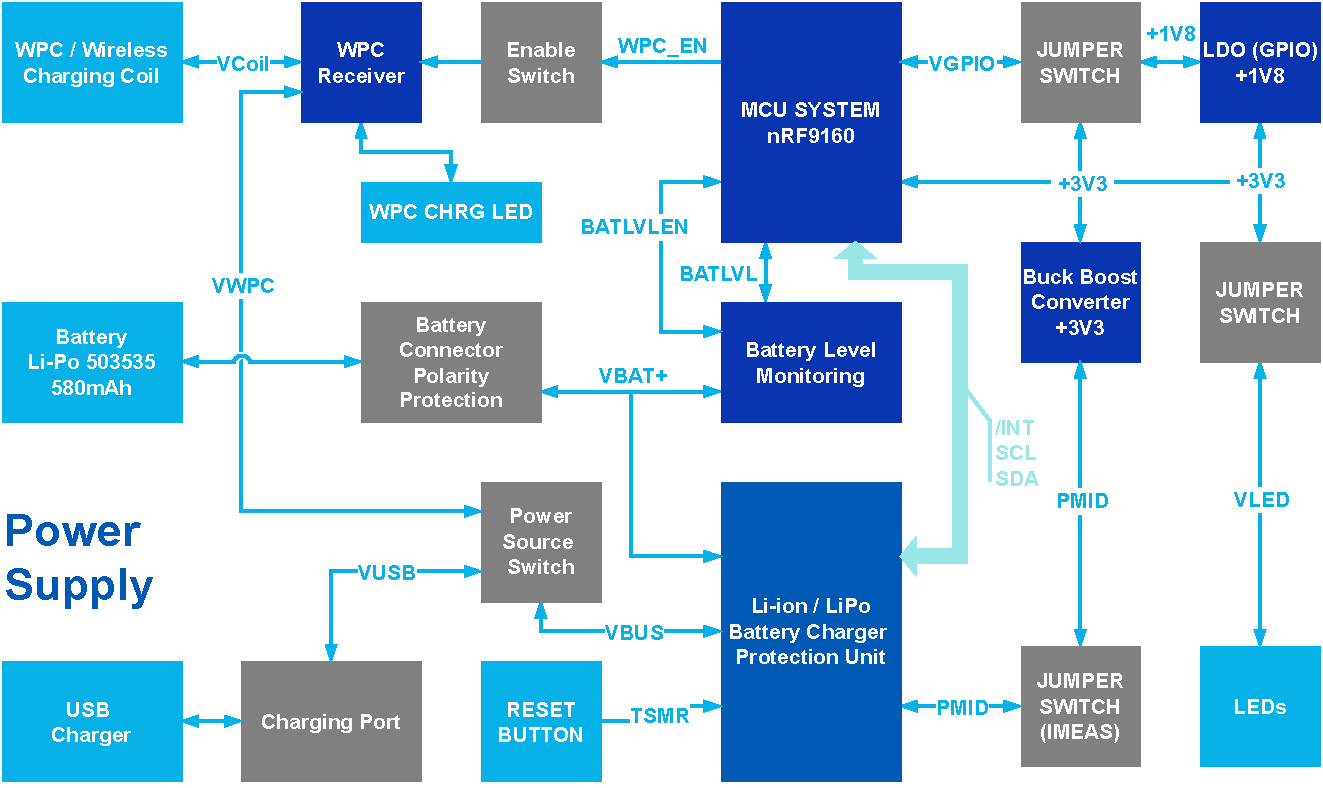
\includegraphics[width=1\textwidth]{Include/Figure/Hardware/power_supply_blk.pdf}
	\caption{Power Supply Block Diagram}
	\label{fig:power_supply_blk}
\end{figure}

\pagebreak

\begin{flushleft}
The \textit{Power Supply} block (figure \ref{fig:power_supply_blk}) implement the following features:
\end{flushleft}
\begin{itemize}
\item [\quad\textbf{Battery Power Supply}]\textbf{:}
\begin{itemize}
	\item Battery connector with ESD and polarity protection circuit
	\item Li-ion/Lipo battery charger and protection unit
	\item Battery level monitoring circuit
\end{itemize}
\item [\quad\textbf{Charging Power Supply}]\textbf{:}
\begin{itemize}
	\item Wireless power coil input with a \textit{WPC} receiver unit
	\item USB-C port to charge the battery and power the system
\end{itemize}
\item [\quad\textbf{System Power Supply}]\textbf{:}
\begin{itemize}
	\item \SI{+3.3}{\volt} buck boost converter to power the system
	\item \SI{+1.8}{\volt} LDO regulator that can be used to power the GPIO of the system
\end{itemize}
\item [\quad\textbf{User Interface}]\textbf{:}
\begin{itemize}
	\item Leds to indicate if the board is ON and if the WPC charge is ON
	\item A master reset push button
	\item A power system jumper to measure the current consumption of the system
\end{itemize}
\end{itemize}

\subsection{User Interface Block Diagram} \label{sec:usr_int_blk_dgr}
The \textit{User Interface} block is a pretty simple, it consists of four push-buttons that will be the only user input available on the smart-watch and also an accelerometer that can be useful to add more functionality to the device. Accelerometer can be use to set a specific profile (normal, sport, etc...), it can also be used to wake-up the system or as a user input.\\

Figure \ref{fig:user_interface_blk} illustrates the \textit{User Interface} block:

\begin{figure}[H]
	\centering
	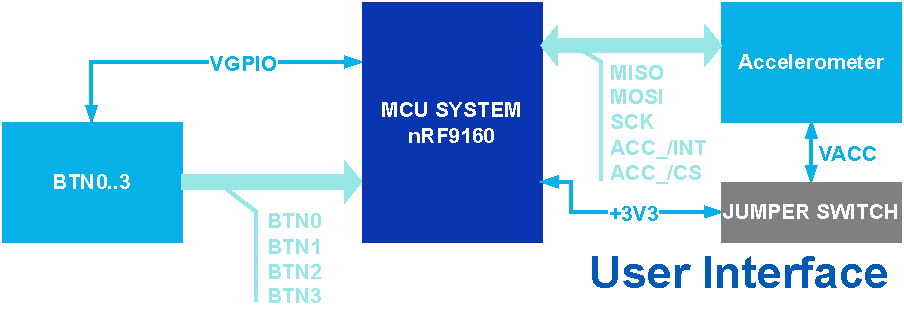
\includegraphics[width=0.8\textwidth]{Include/Figure/Hardware/user_interface_blk.pdf}
	\caption{User Interface Block Diagram}
	\label{fig:user_interface_blk}
\end{figure}

\begin{flushleft}
The \textit{User Interface} block (figure \ref{fig:power_supply_blk}) implement the following features:
\end{flushleft}
\begin{itemize}
\item [\quad\textbf{\textit{BTN} module}]\textbf{:}
\begin{itemize}
\item Four push-buttons that are directly connected to the \textit{nRF9160} (MCU)
\end{itemize}
\item [\quad\textbf{\textit{Accelerometer} module}]\textbf{:}
\begin{itemize}
\item Accelerometer that is connected to the \textit{nRF9160} with a SPI bus
\item Jumper to enable/disable the power supply of the acceleromter to reduce consumption if not implemented.
\end{itemize}
\end{itemize}

\section{Data Display Block Diagram} \label{sec:disp_blk_dgr}
The \textit{Data Display} block contains all the "graphical" user interface (\textit{GUI}). Information such as the time is displayed on a clock with three hands ($h:m:s$). This clock is driven by three miniaturized stepper motors. A small LCD screen is also implemented to display more complex information, such as network reception status, date, battery level or charging status, as well as text.\\

Figure \ref{fig:data_display_blk} illustrates the \textit{Data Display} block diagram:

\begin{figure}[H]
	\centering
	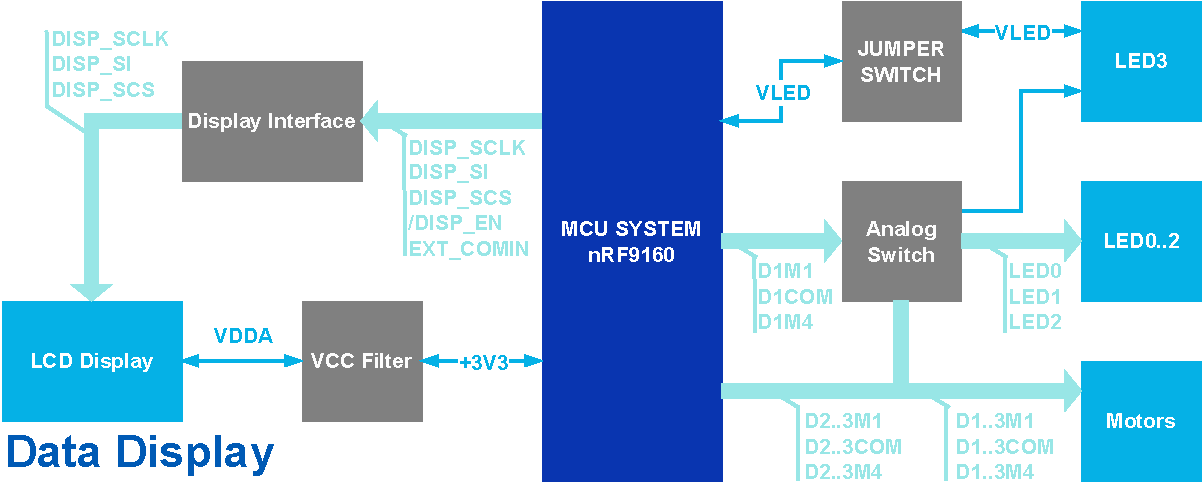
\includegraphics[width=1\textwidth]{Include/Figure/Hardware/data_display_blk.pdf}
	\caption{Data Display Block Diagram}
	\label{fig:data_display_blk}
\end{figure}

\begin{flushleft}
The \textit{Data Display} block shown in figure \ref{fig:data_display_blk} includes the following features:
\end{flushleft}
\begin{itemize}
\item  [\quad\textbf{\textit{LCD Display} module}]\textbf{:}
\begin{itemize}
\item The LCD is driven by the system MCU (\textit{nRF9160}) through the display interface circuit
\item The \textit{Sharp Memory In Pixel} LCD module is sensitive to noise on the power supply that is why a \textit{VCC Filter} circuit is required. 
\end{itemize} 
\item [\quad\textbf{\textit{Motors} module}]\textbf{:}
Used to display the time with three miniaturized stepper motors. One stepper motor is dedicated to the \textit{hours}, one to the \textit{minutes} and the last one to the \textit{seconds}. The position of each stepper motor is driven by two coils which require three command signals:
\begin{enumerate}
\item DxM1 : Independent side of coil A
\item DxCOM : Common side between the two coils A and B
\item DxM4 : Independent side of coil B
\end{enumerate}
\item [\quad\textbf{\textit{LED} modules:}]\textbf{:}
To make debugging easier, the three command signal of motor D1 can be redirected on three leds (\textit{LED0}, \textit{LED1} ,\textit{LED2}) \textit{LED3} indicate if debugging leds are used or not:
\begin{enumerate}
\item \textbf{\textit{LED3}} is \textbf{ON} if debbugging leds are used.
\item \textbf{\textit{LED3}} is \textbf{OFF} if motor D1 is used.
\end{enumerate}
\end{itemize}

\subsection{RF Communication Block Diagram} \label{sec:rf_blk_dgr}
The \textit{RF Communication} block is very important because it contains the main  features of the \textit{LTEWatch} which are \textit{LTE-M/NB-IoT} reception and transmission (\textit{MQTT}) and {GNSS} signal reception for position tracking and smart-watch time accuracy.\\

The \textit{nRF9160} System-in-Package (SiP) is available with and without an integrated \textit{GNSS} receiver module. The SiP with integrated \textit{GNSS} module allows the use of software libraries directly from \textsc{Nordic Semi} which facilitates its implementation.
The biggest disadvantage of this solution is that the modem of the \textit{nRF9160} cannot simultaneously use the integrated \textit{GNSS} module and the \textit{LTE-M/NB-IoT} module. This is a significant constraint that reduces system performance.\\

 For this reason, the choice was made to use the SiP without an integrated \textit{GNSS} module and to implement an external one that interfaces with the MCU system (\textit{nRF9160}) using a serial bus.\\
 
To speed up the development, the \textit{LTE-M/NB-IoT} reception and transmission line is identical to the \textit{nRF9160DK} (development kit) and uses the same antenna.\\

Both \textit{GNSS} and \textit{LTE-M/NB-IoT} can be connected to on-board antenna and external antenna with SMA connectors.\\

Figure \ref{fig:rf_communication_blk} illustrates the \textit{RF Communication} block diagram:

\begin{figure}[H]
	\centering
	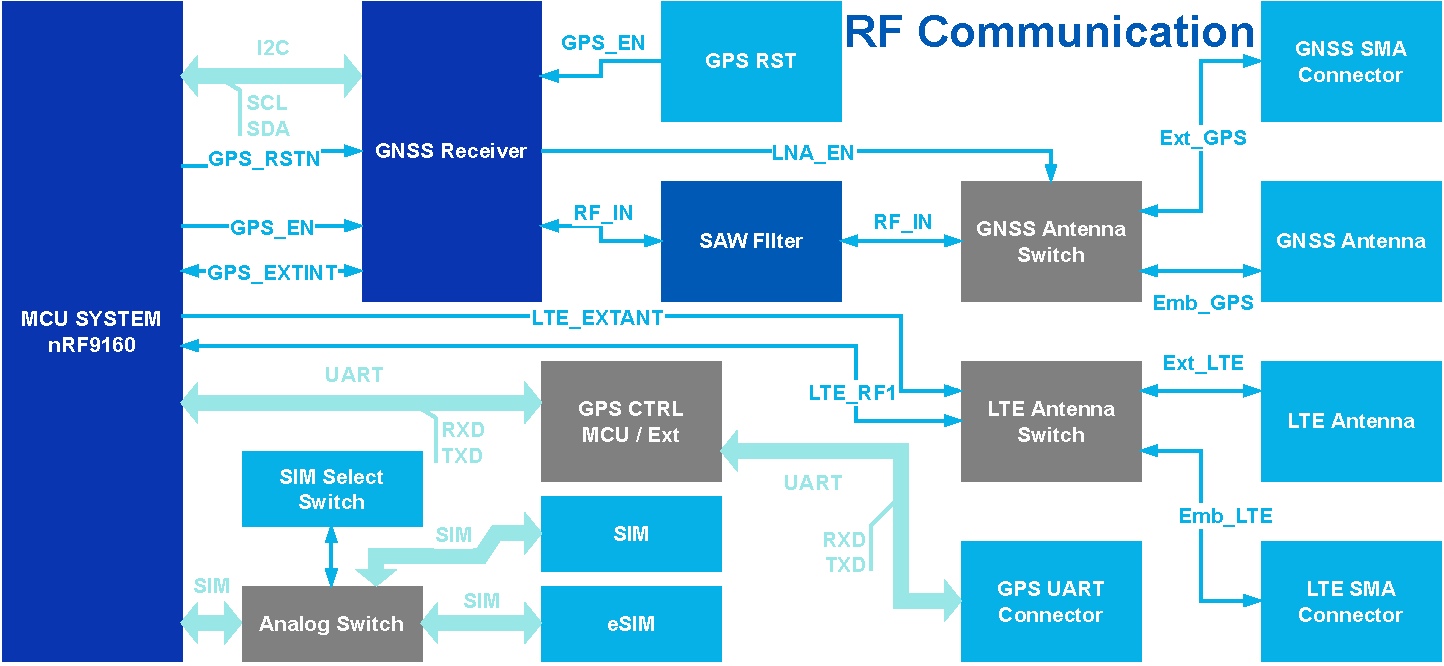
\includegraphics[width=1\textwidth]{Include/Figure/Hardware/rf_communication_blk.pdf}
	\caption{RF Communication Block Diagram}
	\label{fig:rf_communication_blk}
\end{figure}

\pagebreak

\begin{flushleft}
The \textit{RF Communication} block illustrated in figure \ref{fig:rf_communication_blk} includes the following features:
\end{flushleft}
\begin{itemize}
\item [\quad\textbf{\textit{GNSS} reception line with}]\textbf{:}
\begin{itemize}
\item A \textit{GNSS} receiver that communicates with the system MCU by \textit{I2C}. The MCU send three command signals to the \textit{GNSS} receiver:
\begin{enumerate}
\item \textit{GPS\_RSTN} : \textit{GNSS} receiver reset
\item \textit{GPS\_EN} : \textit{GNSS} receiver power supply enable
\item \textit{GPS\_EXTINT} : \textit{GNSS} receiver external interruption
\end{enumerate}
\item An antenna switch to connect the \textit{GNSS} line to on-board antenna or external antenna. This switch is commanded by the \textit{GNSS} receiver \textit{LNA\_EN} output.
\item A SMA connector to connect an external antenna to the board.
\item The \textit{GNSS} receiver can also be interfaced with \textit{UART} bus. This bus can either be connected to system MCU or to an external source by a \textit{UART} bus connector.
\end{itemize}
\item [\quad\textbf{\textit{LTE-M/NB-IoT} reception and transmission line with}]\textbf{:}
\begin{itemize}
\item An antenna switch to connect the \textit{LTE-M/NB-IoT} line to on-board antenna or external antenna. The switch is commanded by \textit{LTE\_EXTANT} signal from system MCU.
\item A SMA connector to connect an external antenna to the board.
\end{itemize}
\item [\quad\textbf{\textit{SIM} and \textit{eSIM} card interface}]\textbf{:}
\begin{itemize}
\item The \textit{SIM} card interface automatically select the which card to connect to the system MCU. This interface is identical to the \textit{nRF9160} one. 
\end{itemize} 
\end{itemize}

\pagebreak
\subsection{MCU Programming Block Diagram} \label{sec:mcu_blk_dgr}
The \textit{MCU Programming} block contains all the module required to flash and debug the system MCU \textit{nRF9160}.\\

Figure \ref{fig:mcu_programming_blk} illustrates the \textit{MCU Programming} block:

\begin{figure}[H]
	\centering
	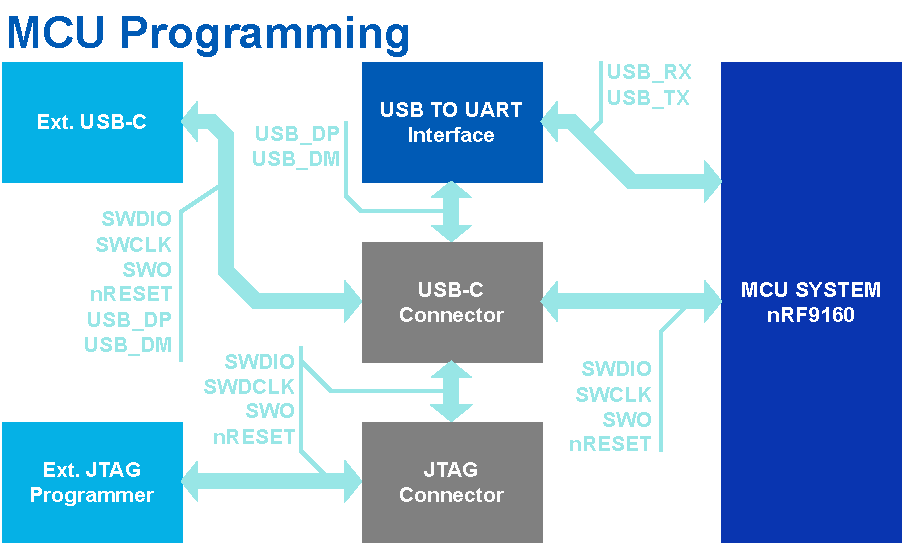
\includegraphics[width=0.8\textwidth]{Include/Figure/Hardware/mcu_programming_blk.pdf}
	\caption{MCU Programming Block Diagram}
	\label{fig:mcu_programming_blk}
\end{figure}

The \textit{MCU Programming} block illustrated in figure \ref{fig:mcu_programming_blk} includes:
\begin{itemize}
\item [\quad\textbf{\textit{USB-C} module}]\textbf{:}
\begin{itemize}
\item Connector to interface system MCU to a programmer with a USB-C programmer. The USB-C programmer was developed for the project \textit{GregTracker} from the HEI (Hes-so Wallis).
\end{itemize} 
\item [\quad\textbf{\textit{Ext. JTAG Programmer} module}]\textbf{:}
\begin{itemize}
\item Connector to interface system MCU with a \textit{Segger J-Link} \textit{JTAG} Programmer or directly to the \textit{nRF9160DK} (development kit) \textit{JTAG} output.
\end{itemize}
\end{itemize}

\pagebreak

\section{LTEWatch Functional Architecture Diagram} \label{sec:ltew_arch_dgr}
The \textit{LTEWatch} system is an assembly of all blocks described in the system breakdown, which are: The \textit{Power Supply} block, the \textit{User Interface} block, the \textit{Data Display} block, the \textit{User Interface} block, the \textit{RF Communication} block and the \textit{MCU Programming} block.\\

The \textit{LTEWatch} overall system functional architecture diagram is illustrated in figure \ref{fig:system_block}:

\begin{figure}[H]
	\centering
	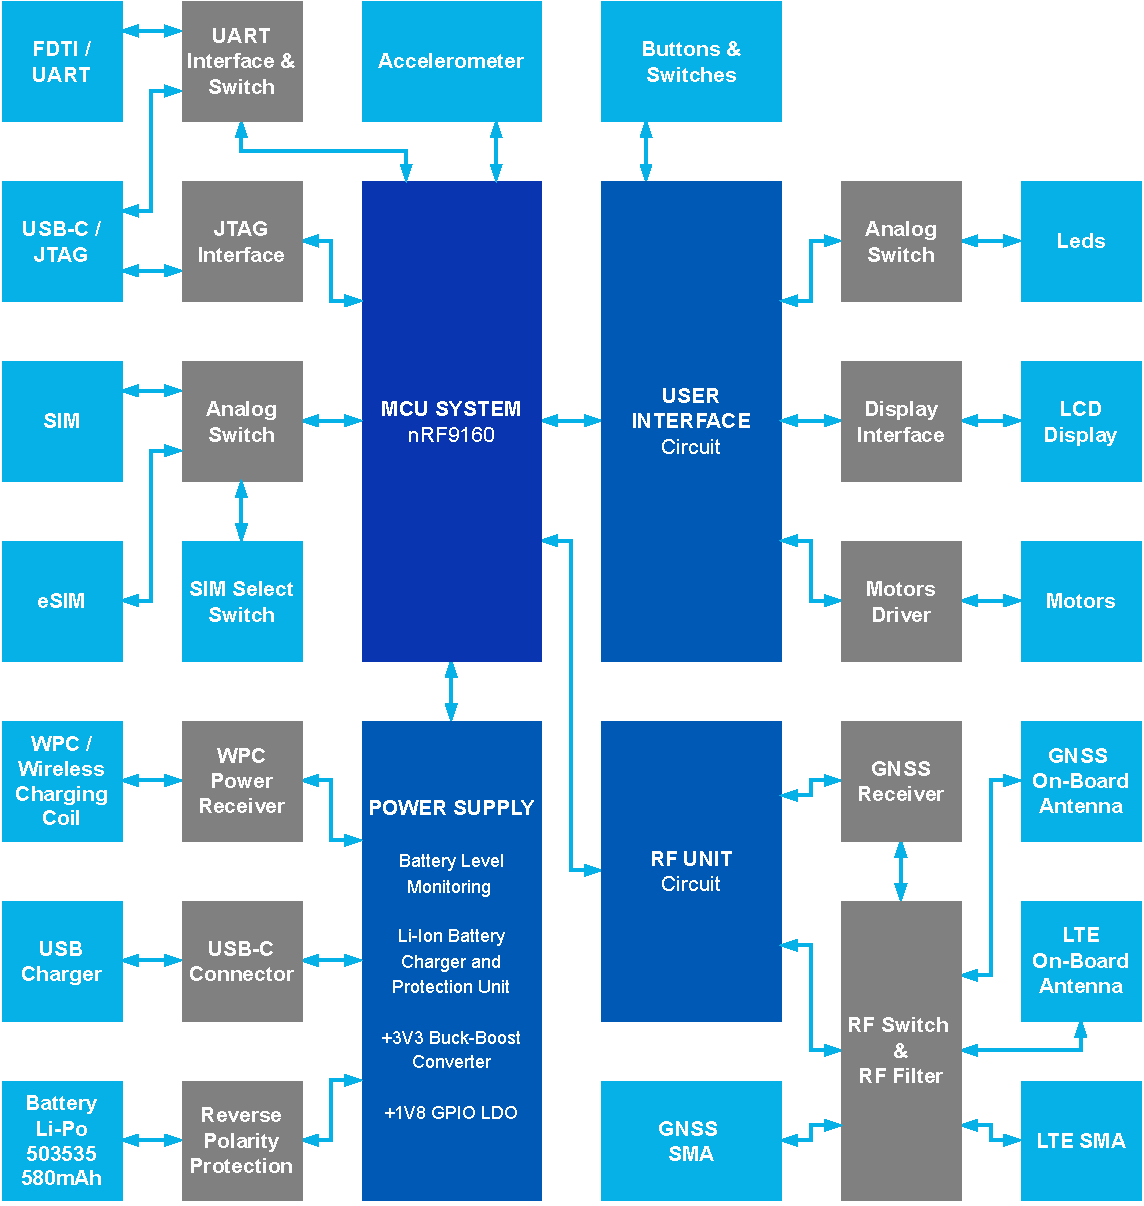
\includegraphics[width=1\textwidth]{Include/Figure/Hardware/system_block.pdf}
	\caption{LTEWatch Block Diagram}
	\label{fig:system_block}
\end{figure}

\pagebreak

\section{LTEWatch Prototype board (PCB) structure} \label{sec:ltew_proto_brd_strct}
The prototype board of \textit{LTEWatch} must allow to validate the implementation of each block described in the system decomposition and must also make it possible to measure and test the performance of the system, i.e. device consumption, an approximation of the system autonomy, the precision of \textit{GPS} tracking as well as the reliability of LTE-M/NB-IoT. This board should also allow experimentation and creation of custom antennas for the \textit{GNSS} receiver and the \textit{LTE} modem.\\

In order to fulfill these conditions, the board must allow to use certain functionality or not, using switch or configurable jumpers, the board must also allow to select the type of antenna used (on-board or external).\\

Figure \ref{fig:board_struct} illustrates the prototype board (PCB) structure:

\begin{figure}[H]
	\centering
	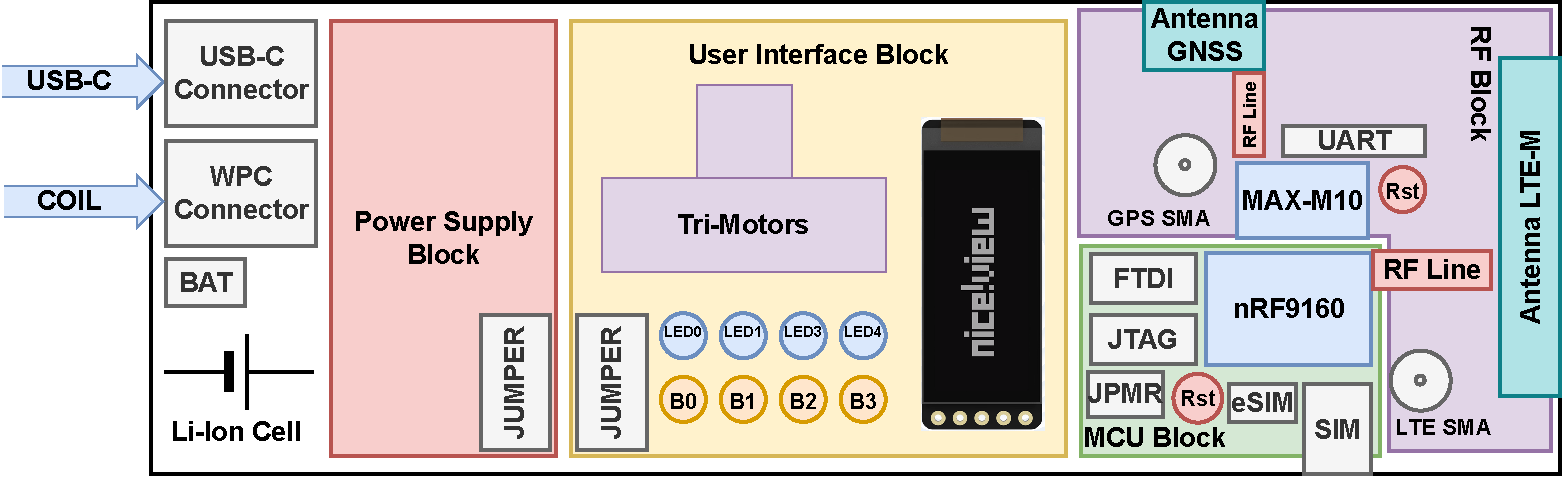
\includegraphics[width=1\textwidth]{Include/Figure/Hardware/board_struct.pdf}
	\caption{Prototype Board PCB Diagram}
	\label{fig:board_struct}
\end{figure}
As seen in figure \ref{fig:board_struct}, the board contains the following blocks:
\begin{enumerate}
\item Power supply connectors:
\begin{itemize}
\item USB-C connector with \textit{UART} enable jumper and \textit{FTDI} USB to UART module
\item Wireless power coil (WPC) connector
\item Battery cell connector
\end{itemize}
\item Power supply block:
\begin{itemize}
\item Battery reverse polarity protection circuit
\item Battery charger module
\item System power supply regulator (+3V3 buck-boost converter and +1V8 LDO regulator)
\item System current consumption measure jumper
\item Board led power supply enable jumper
\item System \textit{VGPIO }(\SI{3.3}{\volt} or \SI{1.8}{\volt}) configuration jumper
\end{itemize}
\pagebreak
\item User interface block:
\begin{itemize}
\item Programmable leds and buttons
\item Motors connector
\item Display connector (\textit{nice!view} 5 pins or \textit{FFC} 10 pins)
\item Display configuration jumpers
\end{itemize}
\item System MCU block:
\begin{itemize}
\item \textit{nRF9061} SiP
\item MCU reset button
\item \textit{JTAG} connector
\item \textit{SIM} and \textit{eSIM} connectors
\item Serial \textit{I2C} and \textit{SPI} jumpers
\end{itemize}
\item RF block:
\begin{itemize}
\item \textit{LTE} RF line switch and \textit{SMA} connector for external antenna
\item \textit{GNSS} receiver SiP with reset button
\item \textit{GNSS} RF line switch and \textit{SMA} connector for external antenna
\end{itemize}
\end{enumerate}

% ------------------------- Component Selection ---------------------------------
\section{Component Selection} \label{sec:comp_sel}
Once the functional decomposition of \textit{LTEWatch} is complete, the next task is to find suitable components to fulfill each block previously described.\\

As \textit{LTEWatch} is a portable device, this implies that the most important system constraints are the autonomy and the compactness of the battery, which translate for the components by consumption and size. Considering those aspects, it seems judicious to focus on fully integrated chip. This has the advantage of drastically reducing the clutter of the circuit, it also reduce circuit complexity and conception time which reduce time to market (\textit{TTM}) or in this case: time to prototype.\\

The most obvious drawback of a fully integrated chip is that such components are usually more expensive. A less obvious disadvantage is that it increases the system's dependence on very specific components and manufacturers, making the circuit very susceptible to component shortages or cancellations, which may require circuitry redesign that may lead to complications. Risk can be minimized by paying attention to the availability of components and the amount of equivalent alternatives that share similar characteristics, footprints, and pinouts or that can be easily adapted.\\

Considering both pros and cons, this solution seems reasonable, especially given the relatively limited time available for the project, which imply that the second most significant criteria for component selection is their availability.\\

\pagebreak

This section is not a detailed description of every components of the system, it focuses more on mains functional blocks of \textit{LTEWatch}, which are the following:

\begin{enumerate}
\item \textbf{System MCU} : \textit{nRF9160}
\item \textbf{Li-ion/LiPo Battery management unit}: \textit{BQ25180}
\item \textbf{Buck Boost Converter (+3V3)}: \textit{TPS63036}
\item \textbf{LDO Regulator (+1V8)}: \textit{TPS7A03}
\item \textbf{Wireless Power (WPC/QI) Receiver}: \textit{BQ51013B}
\item \textbf{LCD Display}: \textit{LS011B7DH03}
\item \textbf{GNSS Receiver}: \textit{u-blox MAX-M10S}
\item \textbf{FTDI USB To UART Interface:} \textit{FT234XD} (USB to BASIC UART IC)
\item \textbf{GNSS Antenna}: \textit{DUO mXTENDTM (NN03-320)}
\item \textbf{LTE-M/NB-IOT Antenna}: \textbf{P822602} (Universal Broadband FR4 Embedded LTE/LPWA Antenna)
\item \textbf{Clock Motors}: \textit{TITAN T901A/T902A}
\end{enumerate}

\subsection{Li-ion/LiPo Battery management unit - BQ25180}
\subsubsection{Description:}
As describe in its datasheet, the \textit{BQ25180}\cite{bq25180DS} is a single cell Li-ion/Lipo battery charger in a very small \textit{DSBGA} package ($\SI{1.6}{\milli\meter}\times\SI{1.1}{\milli\meter}$), a low quiescent current, up to \SI{1}{\ampere} charging and up to \SI{2.5}{\ampere} system loads.

\subsubsection{Typical Application Diagram:}

Figure \ref{fig:bq25180_simplified_schematic} illustrates the simplified schematic of  \textit{BQ25180} battery charger:

\begin{figure}[H]
	\centering
	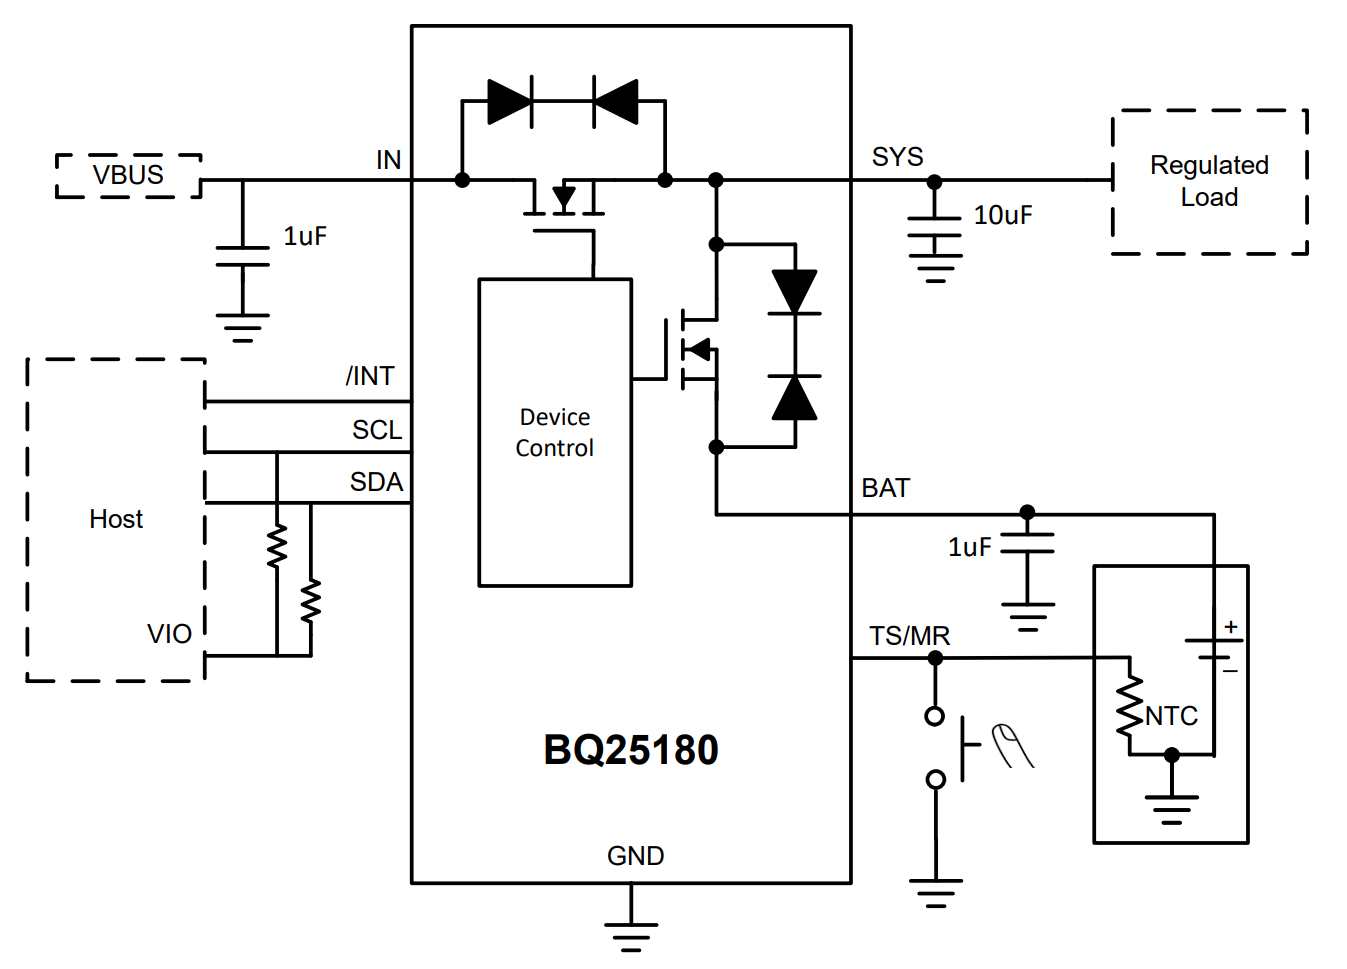
\includegraphics[width=0.7\textwidth]{Include/Figure/comp/bq25180_simplified_schematic.png}
	\caption{Simplified Schematic - Source: \textit{BQ25180}\cite{bq25180DS}}
	\label{fig:bq25180_simplified_schematic}
\end{figure}

The typical application diagram shown in figure \ref{fig:bq25180_simplified_schematic} shows that the implementation of \textit{BQ25180} is very simple and really limits the number of external components needed. This is very positive with regard to the size constraints of wearable devices. Fully programmable settings allow for greater system flexibility and easy battery changes. The downside of programmable settings is extra work during software development as it requires to implement an \textit{I2C} bus and a compatible driver to interface with \textit{BQ25180}.

\subsubsection{Features:}
The \textit{BQ25180}\cite{bq25180DS} battery charger main features are the following:
\begin{itemize}
\item \textbf{Settings:} fully programmable by \textit{I2C} serial bus
\item One push-button wake-up and reset input
\item \textbf{Consumption:}
\begin{itemize}
\item Ultra low quiescent current modes:
\begin{itemize}
\item \SI{15}{\nano\ampere} \textit{Shutdown} mode
\item \SI{3.2}{\micro\ampere} \textit{Ship} mode with button press wake
\item \SI{3}{\micro\ampere} in \textit{Battery Only} mode
\item \SI{30}{\micro\ampere} input adapter $Iq$ in \textit{Sleep} mode
\end{itemize}
\end{itemize}
\item \textbf{Battery protection:}
\begin{itemize}
\item Integrated Power Path (FET) to disconnect the battery
\item Battery under voltage protection (\textit{UVP})
\item Battery over voltage protection (\textit{OVP})
\item Battery short protection
\item Charge and discharge current limitation
\item Battery thermal fault protection
\end{itemize}
\item \textbf{System protection:}
\begin{itemize}
\item Thermal regulation and thermal shutdown
\item Watchdog and safety timer fault
\item Input over-voltage protection
\item System short protection
\item System over-voltage protection
\end{itemize}
\item \textbf{Size:} 8-pin chip in \textit{DSBGA} package ($\SI{1.6}{\milli\meter}\times\SI{1.1}{\milli\meter}$)\\
\end{itemize}

The biggest advantage of the \textit{BQ25180} battery charger is the integrated power path, which means that external MOSFETs for battery protection are not required and the management of system powering and battery charging is already implemented. This greatly reduces circuit complexity and component count. The \textit{BQ25180} also has a very low consumption with a quiescent current of only \SI{3}{\micro\ampere} when in \textit{Battery Only} mode.

\subsubsection{Absolute Maximum Ratings:}
The table \ref{tab:bq25180_absolute_max_rating} shows the absolute maximum ratings of the \textit{BQ25180}:

\begin{table}[H]
\centering
\begin{tabularx}{\textwidth}{|X|l|c|c|c|}
\hline
\, & \; & \textbf{MIN} & \textbf{MAX} & \textbf{UNIT} \\\hline
Input Voltage & IN & $-0.3$ & $25$ & $\si{\volt}$ \\\hline
Voltage & All other pins & $-0.3$ & $5.5$ & $\si{\volt}$ \\\hline
Input Current (DC) & IN & & $1.1$ & $\si{\ampere}$ \\\hline
SYS Discharge Current (DC) & SYS & & $1.5$ & $\si{\ampere}$ \\\hline
SYS Discharge Curr. ($t_{pulse}<\SI{20}{\milli\second}$) & SYS & & $2.5$ & $\si{\ampere}$ \\\hline
Output Sink Current & /INT & & $20$ & $\si{\milli\ampere}$ \\\hline
$T_J$ & Junction temp. & $-40$ & $150$ & $\si{\celsius}$ \\\hline
$T_{stg}$ & Storage temp. & $-65$ & $150$ & $\si{\celsius}$ \\\hline
\end{tabularx}
\caption{Absolute Maximum Ratings - Source: \textit{BQ25180}\cite{bq25180DS}}
\label{tab:bq25180_absolute_max_rating}
\end{table}

\subsubsection{Recommended Operating Conditions:}
The table \ref{tab:bq25180_recom_oper_cond} shows the recommended operation conditions of the \textit{BQ25180}:

\begin{table}[H]
\centering
\begin{tabularx}{\textwidth}{|l|X|c|c|c|}\hline
\textbf{ID} & \textbf{Description} & \textbf{MIN} & \textbf{MAX} & \textbf{UNIT} \\\hline
VBAT & Battery Voltage Range & $2.2$ & $4.6$ & $\si{\volt}$ \\\hline
VIN & Input Voltage Range & $2.7$&  $5.5$ & $\si{\volt}$ \\\hline
IIN & Input Current Range (IN to SYS) & & $1.1$  & $\si{\ampere}$ \\\hline
IBAT & Battery Discharge Current (BAT to SYS) & & $1.5$ & $\si{\ampere}$ \\\hline
TJ & Operating Junction Temperature Range & $-40$ & $125$ & $\si{\celsius}$ \\\hline
\end{tabularx}
\caption{Recommended operating conditions - Source: \textit{BQ25180}\cite{bq25180DS}}
\label{tab:bq25180_recom_oper_cond}
\end{table}

\subsubsection{Design Recommendations:} \label{sec:bat_chrg_sel}
The \textit{BQ25180} implementation is relatively easy, however the datasheet provides some design recommendations that are important to have in mind.\\

According to the datasheet\cite{bq25180DS}:
\begin{enumerate}
\item \textbf{Input decoupling (IN/SYS) Capacitors:}
\begin{itemize}
\item Prefer low \textit{ESR} ceramic capacitors such as \textit{X7R} or \textit{X5R}.
\item Must be placed as close as possible to \textit{VCC} and \textit{groundGND} pins.
\item It is recommended to use \SI{25}{\volt} rated capacitors due to their derating voltage.
\item The minimum capacitance after derating must by higher than \SI{1}{\micro\farad}.
\end{itemize}
\item \textbf{TS:} The \textit{GND} connection of the \textit{NTC} should be as close as possible to the \textit{GND} pin of the \textit{BQ25180} or thermally connected to it. This is to minimize any error in TS measurement due to temperature drop in the ground plane of the board.
\item \textbf{Recommended Passive Components:}\\
The recommended values of the passive components are given in table \ref{tab:bq25180_recom_pass_comp}:
\begin{table}[H]
\centering
\begin{tabularx}{0.9\textwidth}{|l|X|c|c|c|c|}\hline
\textbf{ID} & \textit{Description} & \textbf{MIN} & \textbf{NOM} & \textbf{MAX} & \textbf{UNIT}\\\hline
$C_{SYS}$	& Capacitance on SYS pin & $1$ & $10$ & $100$ & $\si{\micro\farad}$\\\hline
$C_{BAT}$ 	& Capacitance on BAT pin & $1$ & $1$ & - & $\si{\micro\farad}$\\\hline
$C_{IN}$ 	& IN input bypass capacitance & $1$ & $1$ & $10$ & $\si{\micro\farad}$\\\hline
\end{tabularx}
\caption{Recommended Passive Components - Source: \textit{BQ25180}\cite{bq25180DS}}
\label{tab:bq25180_recom_pass_comp}
\end{table}
\end{enumerate}

%-------------------------------------------------------------------------------------

\subsection{Buck Boost Converter (+3V3) - TPS63036}

The \textit{MCU} system and all device peripherals need \SI{3.3}{\volt} power, so this component is a critical module in the system. There are many voltage regulator solutions available in the market, but the buck-boost converter has the big advantage of being able to step down and step up the supply voltage to \SI{3.3}{\volt}. This means that with a buck-boost, it is possible to continue using the battery when its voltage is lower than \SI{3.3}{\volt}.\\

To protect the battery, the over-discharge protection unit must disconnect the battery from the system to prevent its voltage from dropping below \SI{3.0}{\volt}. This value depends on the specific characteristics of each battery, but \SI{3.0}{\volt} is a safe value for most Li-ion cells. Thus, with a buck-boost converter solution, the battery voltage range between \SI{3.0}{\volt} and \SI{3.3}{\volt} can still be used to power the system, this represents a valuable additional autonomy.

\subsubsection{Typical Application Diagram:}

Figure \ref{fig:tps63036_simplified_schematic} illustrates typical application schematic of \textit{TPS63036}:

\begin{figure}[H]
	\centering
	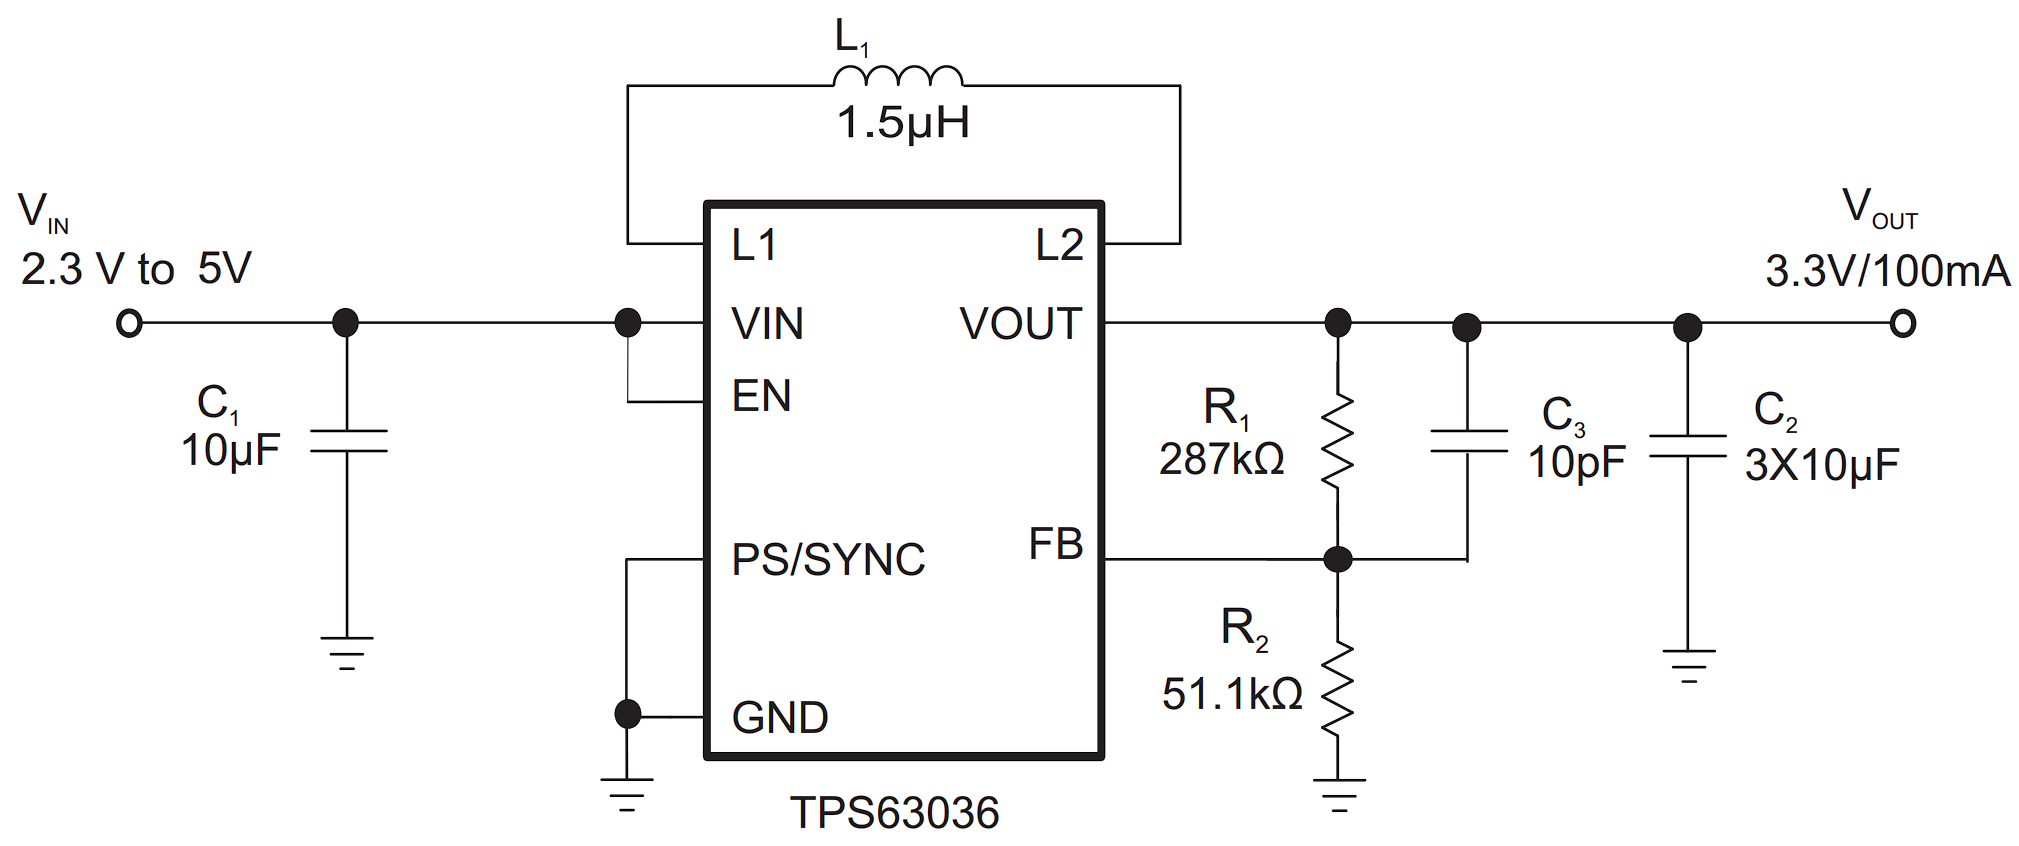
\includegraphics[width=0.9\textwidth]{Include/Figure/comp/tps63036_simplified_schematic.png}
	\caption{Typical application schematic - Source: \textit{TPS63036}\cite{TPS63036}}
	\label{fig:tps63036_simplified_schematic}
\end{figure}

\pagebreak

\subsubsection{Description:}

As describe in its datasheet, the \textit{TPS63036}\cite{TPS63036} is non-inverting buck-boost converter based on a fixed frequency (\textit{PWM}) controller using synchronous rectification to increase efficiency. The high efficiency is also maintain over a wide load current range by entering in power save mode when the load current is low. The maximum output current is limited to a typical value of \SI{1}{\ampere}. The output voltage is programmable using external resistor divider. To minimize battery drain, the converter can also be disable and the load is disconnected from the supply during shutdown.

\subsubsection{Features:}

According to the datasheet of the \textit{TPS63036}\cite{TPS63036} converter:
\begin{itemize}
\item \textbf{Performances:}
\begin{itemize}
	\item Input voltage from \SI{1.8}{\volt} to \SI{5.5}{\volt}
	\item Adjustable output voltage from \SI{1.2}{\volt} to \SI{5.5}{\volt}
	\item High efficiency over entire load range
\end{itemize}
\item \textbf{Consumption}
\begin{itemize}
	\item Low operating quiescent current: \SI{25}{\micro\ampere}
	\item Power save mode available
\end{itemize}
\item \textbf{Safety and protection features:}
\begin{itemize}
\item Over-temperature protection
\item Over-voltage protection
\item Load disconnect during shutdown
\end{itemize}
\item \textbf{Size:} 8-pin chip in \textit{WCSP} package ($\SI{1.814}{\milli\meter} \times \SI{1.076}{\milli\meter}$)
\end{itemize}

\subsubsection{Efficiency vs Output Current:}

Figure \ref{fig:tps63036_simplified_schematic} illustrates the graph of efficiency vs output current of the \textit{TPS63036}:

\begin{figure}[H]
	\centering
	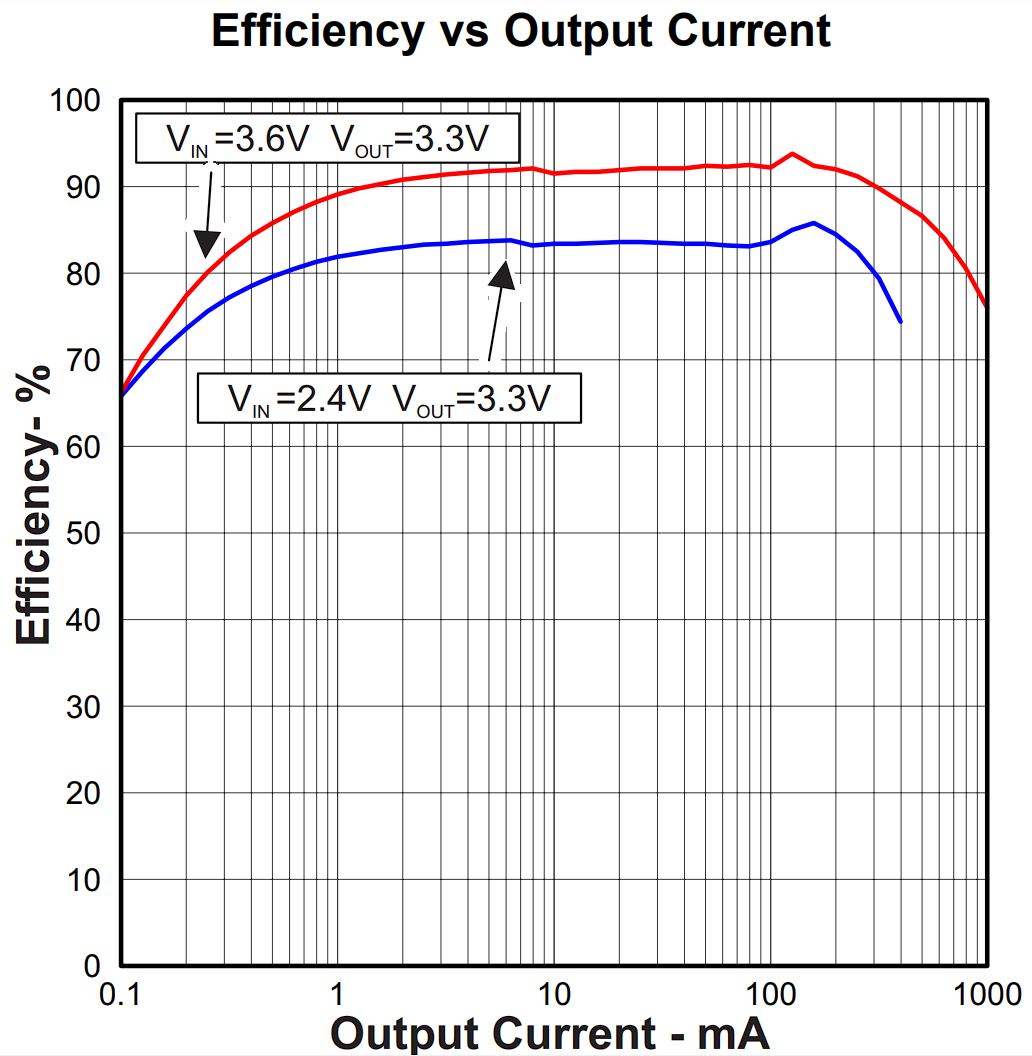
\includegraphics[width=0.45\textwidth]{Include/Figure/comp/tps63036_efficiency_output_current.png}
	\caption{Efficiency vs Output Current Graph - Source: \textit{TPS63036}\cite{TPS63036}}
	\label{fig:tps63036_efficiency_output_current}
\end{figure}

Figure \ref{fig:tps63036_efficiency_output_current} shows that the \textit{TPS63036}\cite{TPS63036} maintains relatively good performance over a wide range of load current consumption:
$$
\mathlarger{\eta} =
\begin{cases} 
\quad >\SI{90}{\percent} \quad : \quad \SI{1.5}{\milli\ampere} < I_{Load} < \SI{1.5}{\milli\ampere} \\
\quad >\SI{80}{\percent} \quad : \quad \SI{250}{\micro\ampere} < I_{Load} < \SI{800}{\milli\ampere}
\end{cases}
$$


\subsubsection{Absolute Maximum Ratings:}

The table \ref{tab:tps63036_abs_max} shows the absolute maximum ratings given by the datasheet of the \textit{TPS63036}\cite{TPS63036}:

\begin{table}[H]
\centering
\begin{tabularx}{\textwidth}{|X|c|c|c|}\hline
\textbf{Description} & \textbf{MIN} & \textbf{MAX} & \textbf{UNIT} \\\hline
Input voltage on $VIN$, $L1$, $L2$, $VOUT$, $PS/SYNC$, $EN$, $FB$ & $-0.3$ & $7$ & $\si{\volt}$ \\\hline
Operating virtual junction temperature, $T_J$ & $-40$ & $150$ & $\si{\celsius}$ \\\hline 
Storage temperature, $T_{stg}$ & $-65$ & $150$ & $\si{\celsius}$ \\\hline 
 
\end{tabularx}
\caption{Absolute Maximum Ratings - Source: \textit{TPS63036}\cite{TPS63036}}
\label{tab:tps63036_abs_max}
\end{table}

\subsubsection{Recommended Operating Conditions:}

The table \ref{tab:tps63036_recom_op} shows recommended operating conditions according to the datasheet of the \textit{TPS63036}\cite{TPS63036}:

\begin{table}[H]
\centering
\begin{tabularx}{\textwidth}{|X|c|c|c|}\hline
\textbf{Description} & \textbf{MIN} & \textbf{MAX} & \textbf{UNIT} \\\hline
Supply voltage at $VIN$ & $1.8$ & $5.5$ & $\si{\volt}$ \\\hline
Operating free air temperature, $T_A$ & $-40$ & $85$ & $\si{\celsius}$ \\\hline 
Operating virtual junction temperature, $T_J$, $T_{stg}$ & $-40$ & $125$ & $\si{\celsius}$ \\\hline 
 
\end{tabularx}
\caption{Recommended Operating Conditions - Source: \textit{TPS63036}\cite{TPS63036}}
\label{tab:tps63036_recom_op}
\end{table}

\subsubsection{Design Recommendations:} \label{sec:bck_bst_sel}
The datasheet of the \textit{TPS63036}\cite{TPS63036} provides design guideline for external components selection. The next sections will follow this guideline for the \textit{LTEWatch} application. For more detailed information, refers to the datasheet of the \textit{TPS63036}\cite{TPS63036}. 

\subsubsection{Output Filter Recommendations:}

\begin{itemize}[\;]
\item Buck-boost converter have a very noisy output that need to be smoothed with an output filter in order to provide a usable power supply for the load system. Therefore, this filter must be compatible with the internal loop compensation of the \textit{TPS63036}. The datasheet provide the following recommendations:
\begin{enumerate}
\item The external filter should be a $L-C$ filter.
\item Low limit condition for the inductor is: $\underline{\underline{L \geq \SI{1}{\micro\farad}}}$. Below this limit, subharmonic oscillation can appear.
\end{enumerate}
The table \ref{fig:TPS63036_output_capacitor_filter} provide possible $L$ and $C$ value combinations:
\begin{figure}[H]
	\centering
	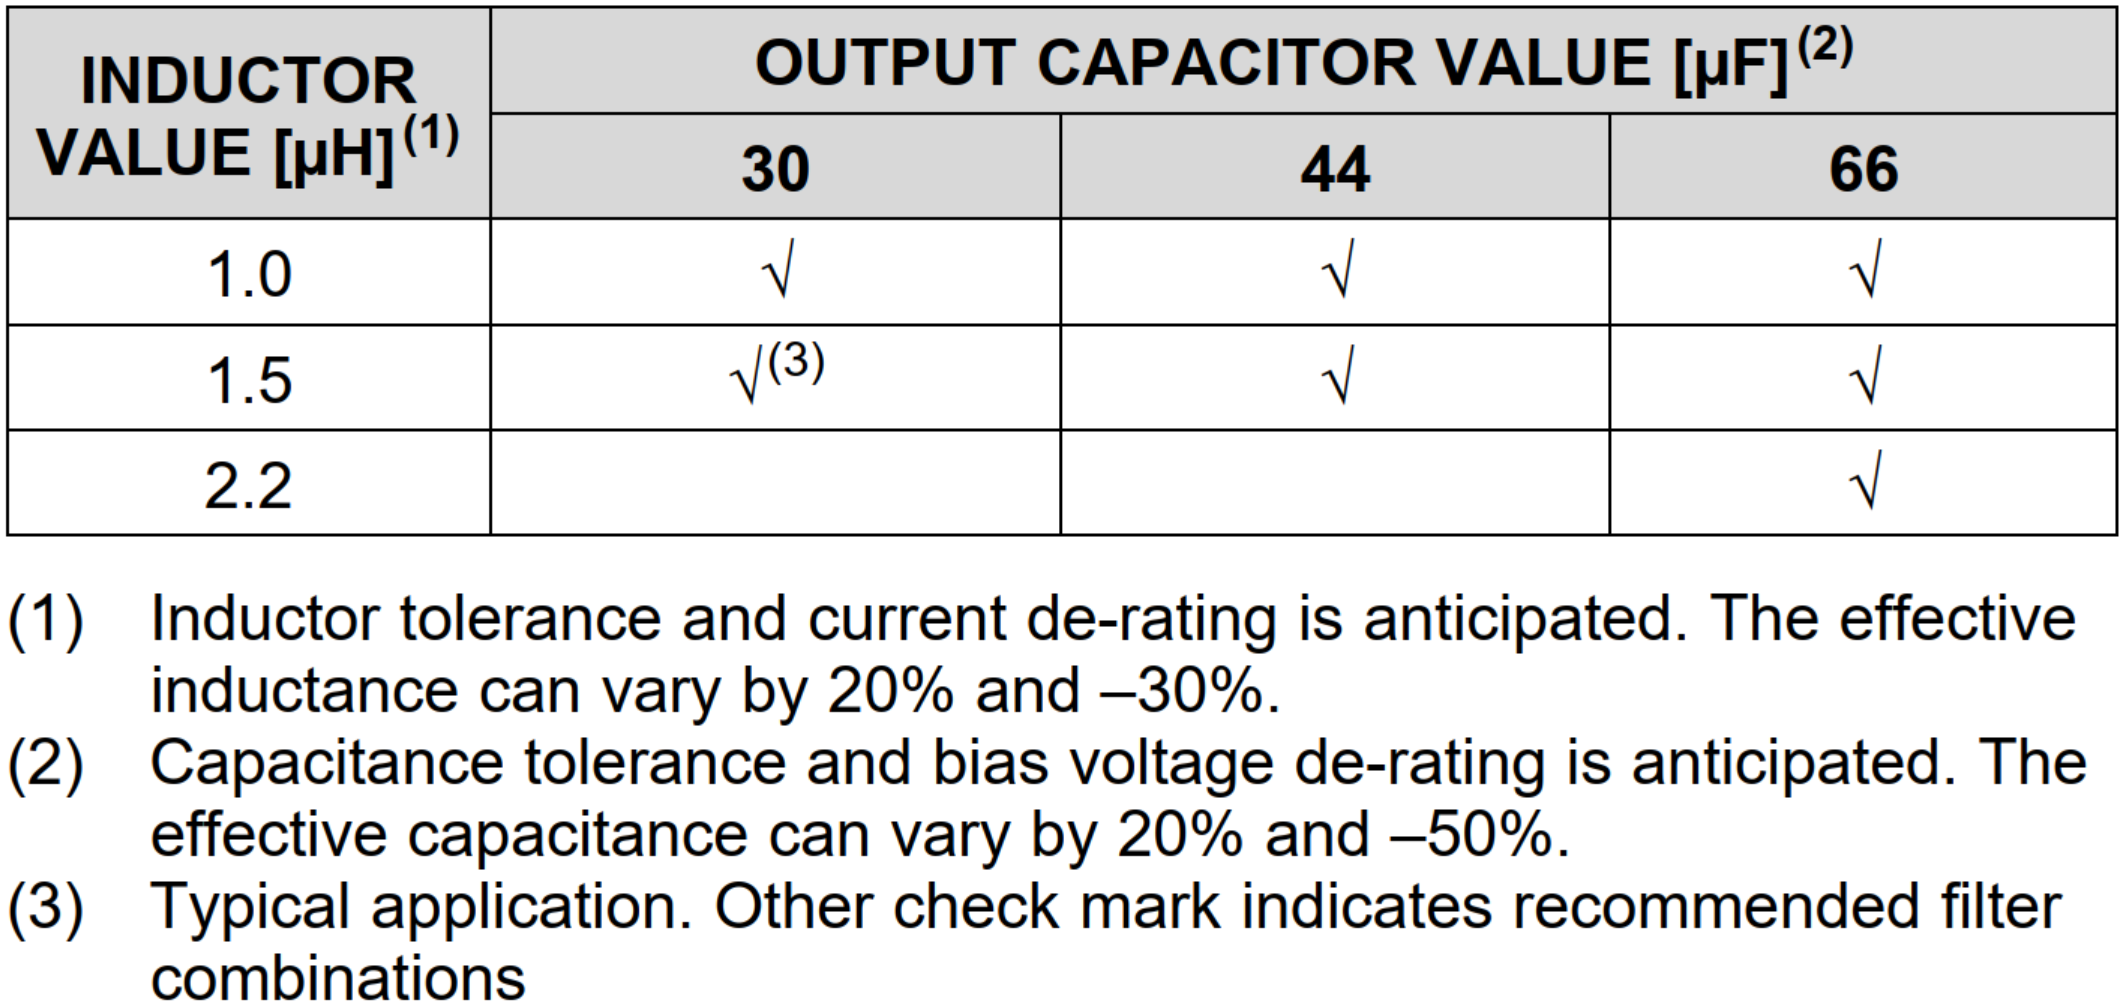
\includegraphics[width=0.8\textwidth]{Include/Figure/comp/TPS63036_output_capacitor_filter.png}
	\caption{Output Filter Selection (Current up to \SI{1}{\ampere}) - Source: \textit{TPS63036}\cite{TPS63036}}
	\label{fig:TPS63036_output_capacitor_filter}
\end{figure}
\end{itemize}


\subsubsection{Inductor Selection:}

\begin{enumerate}
\item Select inductor with a low DC resistance to minimize conduction loss
\item Avoid saturation of the inductor by calculating the peak current in steady-state operation (eq. \ref{eq:TPS63036_ind}):

\begin{equation}
\label{eq:TPS63036_ind}
\boxed{\begin{array}{l l}
\text{Duty Cycle Boost:} & D = \dfrac{V_{out}-V_{in}}{V_{out}} \\
\text{Peak current:} & I_{PEAK} = I_{SW\_MAX} + \dfrac{V_{in} \cdot D}{2 \cdot f \cdot L}
\end{array}}
\end{equation}

Where:

\begin{center}
\begin{tabular}{r l}
$D$: & Duty cycle in boost mode\\
$f$: & Converter switching frequency (typ. \SI{2}{\mega\hertz})\\
$L$: & Selected inductor value\\
$\eta$: & Estimated converter efficiency (typ. \SI{80}{\percent})\\
$I_{SW\_MAX}$: & Maximum average input current\\
$V_{out}$: & Output voltage\\
$V_{in}$: & Minimum input voltage\\
\end{tabular}
\end{center}

The \textit{LTEWatch} application uses \textit{Li-Ion/Li-Po} battery as power supply, therefore the worst case is equivalent to a nearly empty battery. To keep some headroom, we can use the extreme value: 

$$ V_{in} = V_{BAT,EMPTY} = \ddl{3.0\si{\volt}} $$

The maximum average input current correspond to the maximal discharge current of the battery. To stay safe for most \SI{500}{\milli\ampere\hour} to \SI{1000}{\milli\ampere\hour} lithium battery, we can use a maximum discharge current:

$$ I_{BAT,DCHRG}= I_{SW\_MAX} = \ddl{500\si{\milli\ampere}}$$

\textit{LTEWatch} boost duty cycle:

$$
D = \dfrac{V_{out}-V_{BAT,EMPTY}}{V_{out}} = \dfrac{3.3-3.0}{3.3} = \ddl{9.\overline{09}\si{\percent}} 
$$

\textit{LTEWatch} peak current with recommanded inductors from the table \ref{fig:TPS63036_output_capacitor_filter}:

$$
I_{PEAK} = I_{BAT,DCHRG} + \dfrac{V_{BAT,EMPTY} \cdot D}{2 \cdot f \cdot L} = 0.5 + \dfrac{3.0 \cdot 0.\overline{09}}{1 \cdot 2\cdot 10^6 \cdot L}
$$

$$
\begin{array}{l c l}
\rightarrow \; L = 1\si{\micro\henry} & \Rightarrow & I_{PEAK} = \ddl{568\si{\milli\ampere}} \\
\rightarrow \; L = 2.2\si{\micro\henry} & \Rightarrow & I_{PEAK} = \ddl{531\si{\milli\ampere}}
\end{array}
$$

We can see that both inductors generate a very similar peak current around \SI{550}{\milli\ampere}, therefore the selected inductor specification should be:

$$
\boxed{\boxed{
\begin{array}{l}
\circ \; \SI{1}{\micro\henry} < L < \SI{2.2}{\micro\henry}\\[5pt]
\circ \; I_{L,SAT} > \SI{600}{\milli\ampere}
\end{array}}}
$$

\item The inductor can affect the stability of the feedback loop. Texas Instrument recommends to keep $f_{RHPZ} > 400 \si{\kilo\hertz}$ (eq. \ref{eq:TPS63036_frhpz})

\begin{equation}
\label{eq:TPS63036_frhpz}
\boxed{\begin{array}{l l}
f_{RHPZ} = \dfrac{(1-D)^2 \cdot V_{out}}{2 \pi \cdot i_{out} \cdot L} & D: \text{ Duty cycle in boost mode}
\end{array}}
\end{equation}

For the \textit{LTEWatch}:
$$
\begin{array}{l c l}
\rightarrow \; L = 1\si{\micro\henry} & \Rightarrow  & f_{RHPZ} = \dfrac{(1-0.\overline{09})^2 \cdot 4.5}{2 \pi \cdot 0.5 \cdot 1 \cdot 10^{-6}} = \ddl{1.183\si{\mega\hertz}} \\[10pt]
\rightarrow \; L = 2.2\si{\micro\henry} & \Rightarrow & f_{RHPZ} = \dfrac{(1-0.\overline{09})^2 \cdot 4.5}{2 \pi \cdot 0.5 \cdot 2.2 \cdot 10^{-6}} = \ddl{538\si{\kilo\hertz}}
\end{array}
$$

We can see that both inductors satisfy the recommended condition for $f_{RHPZ}$.

\subsubsection{Input Capacitor Selection:}

The datasheet recommends at least a \SI{10}{\micro\farad} ceramic capacitor plassed as close as possible to the \textit{VIN} and \textit{GND} pins of the IC. This capacitor improve the transient behavior of the regulator and \textit{EMI} protection.

\subsubsection{Output Capacitor Selection:}

The datasheet recommends multiple stage of output capacitors starting with a small ceramic capacitor placed as close as possible to the \textit{VOUT} and \textit{GND} pins of the IC followed by a bigger one. The typical output total capacitor value is \SI{30}{\micro\farad} but there is no upper limit. If it is necessary to reduce output voltage ripple and dropout, it is possible to increase the output capacitor value.

\subsubsection{Setting the Output Voltage:}

The \textit{TPS63036} converter require an external resistor divider connected between \textit{VOUT}, \textit{FB} and \textit{GND} to set the output voltage. The resistor divider can be calculated with the equation \ref{eq:TPS63036_vout}.
\begin{equation}
\label{eq:TPS63036_vout}
\boxed{R_1 = R_2 \cdot \bigg(\dfrac{V_{OUT}}{V_{FB}} - 1\bigg) \quad \rightarrow \quad \text{with: } 
\begin{cases}
V_{FB} = 500\si{\milli\volt} \text{ (typ.)}\\
R_2 \leq \SI{100}{\kilo\ohm}
\end{cases}}
\end{equation}


For \textit{LTEWatch} application with $R_2 = 100\si{\kilo\ohm}$ and $V_{OUT} = 3.3\si{\volt}$:
$$
R_1 = R_2 \cdot \bigg(\dfrac{V_{OUT}}{V_{FB}} - 1 \bigg) = 100\cdot 10^3 \cdot \bigg(\dfrac{3.3}{0.5} - 1 \bigg) = \ddl{560\si{\kilo\ohm}}
$$

\subsubsection{Current Limit:}
The \textit{TPS63036} internally limit the average input current to protect the device and the IC. The current limit depends on the input voltage and can be calculated with the equations \ref{eq:TPS63036_ilim}:

\begin{equation}
\label{eq:TPS63036_ilim}
\boxed{\begin{array}{l l}
\text{Duty Cycle Boost} & D = \dfrac{V_{OUT}-V_{IN,BOOST}}{V_{OUT}}\\[10pt]
\text{Maximum Output Current Boost: } & I_{OUT} = \eta \cdot I_{SW} \cdot (1-D)\\[10pt]
\text{Duty Cycle Buck: } & D = \dfrac{V_{OUT}}{V_{IN,BUCK}}\\[10pt]
\text{Maximum Output Current Buck: } & I_{OUT} = \dfrac{\eta \cdot I_{SW}}{D}\\
\end{array}}
\end{equation}

Where:

\begin{center}
\begin{tabular}{r l}
$\eta$: & Estimated converter efficiency (typ. \SI{80}{\percent})\\
$f$: & Converter switching frequency (typ. \SI{2}{\mega\hertz})\\
$L$: & Selected inductor value\\
$I_{SW\_MAX}$: & Maximum average input current\\
$V_{IN,BOOST}$: & Minimum input voltage \\
$V_{IN,BUCK}$: & Maximum input voltage\\[10pt]
\end{tabular}
\end{center}

For \textit{LTEWatch} application:

$$
\begin{array}{l l}
D_{BOOST} = \dfrac{3.3 - 3.0}{3.3} = 0.\overline{09} & \Rightarrow \; I_{OUT,BST} = 0.8 \cdot 0.5 \cdot (1-0.09) = \ddl{\SI{728}{\milli\ampere}}\\[15pt]
 D_{BUCK} = \dfrac{3.3}{4.5} = 0.7\overline{33} & \Rightarrow \; I_{OUT,BUCK} = \dfrac{0.8 \cdot 0.5}{0.7\overline{33}} = \ddl{\SI{1.09}{\ampere}}
\end{array}
$$

\textsc{Nordic Semi} recommended to use a power supply that can withstand at least \SI{500}{\milli\ampere} for the \textit{nRF9160} SiP. We can see that the maximum output current of the \textit{TPS63036} is higher than \SI{500}{\milli\ampere} which is perfect.


\end{enumerate}

%-------------------------------------------------------------------------------------

\subsection{LDO Regulator (+1V8) - TPS7A03}
This component is added to give more flexibility to the prototype board by allowing the possibility to set the voltage of the \textit{GPIOs} of the device to \SI{1.8}{\volt} or \SI{3.3}{\volt}, with a jumper. This component is not very critical and should only be able to deliver sufficient current to the \textit{GPIOs}.

\subsubsection{Description:}

As described in the datasheet, the \textit{TPS7A03}\cite{TPS7A03} is an ultra-small, ultra-low quiescent current low dropout linear regulator (LDO) with an output range of \SI{0.8}{\volt} to \SI{5.0}{\volt} and an output current of \SI{200}{\milli\ampere}. This component is specifically design for compact wearable device like:
\begin{itemize}
\item Wearables electronics
\item Thermostats, smoke and heat detectors
\item Gas, heat, and water meters
\item Blood glucose monitors and pulse oximeters
\item Residential circuit breakers and fault indicators
\item Building security and video surveillance devices
\item \textit{EPOS} card readers
\end{itemize}

\subsubsection{Features:}

\begin{itemize}
\item \textbf{Consumption:}
\begin{itemize}
\item Ultra-low $I_Q$: \SI{200}{\nano\ampere} (typ. even in dropout)
\item Shutdown $I_Q$: \SI{3}{\nano\ampere} (typ.)
\end{itemize}
\item \textbf{Performances:}
\begin{itemize}
\item Excellent transient response (\SI{1}{\milli\ampere} to \SI{50}{\milli\ampere}):
\begin{itemize}[$\circ$]
\item < \SI{10}{\micro\second} settling time
\item \SI{80}{\milli\volt} undershoot
\end{itemize}
\item Input voltage range: \SI{1.5}{\volt} to \SI{6.0}{\volt}
\item Output voltage range:\SI{0.8}{\volt} to \SI{5.0}{\volt} (fixed)
\item Output accuracy: \SI{1.5}{\percent} over temperature
\item Smart enable with integrated pulldown (\textit{LDO} disabled even when the EN pin is left floating)
\item Very low dropout: \SI{270}{\milli\volt} (max) at \SI{270}{\milli\ampere} ($V_{OUT} = \SI{3.3}{\volt}$)
\item Stable with a \SI{1}{\micro\farad} or larger capacitor
\end{itemize}
\item \textbf{Size and available packages:}
\begin{itemize}
\item \textit{X2SON}: $\SI{1.0}{\milli\meter} \times \SI{1.0}{\milli\meter}$
\item \textit{DSBGA}: $\SI{0.64}{\milli\meter} \times \SI{0.64}{\milli\meter}$
\item \textit{SOT23-5}
\end{itemize}
\end{itemize}


\subsubsection{Typical Application Diagram:}

Figure \ref{fig:tps7a03_typ_app} illustrates a typical application circuit for the \textit{TPS7A03}:

\begin{figure}[H]
	\centering
	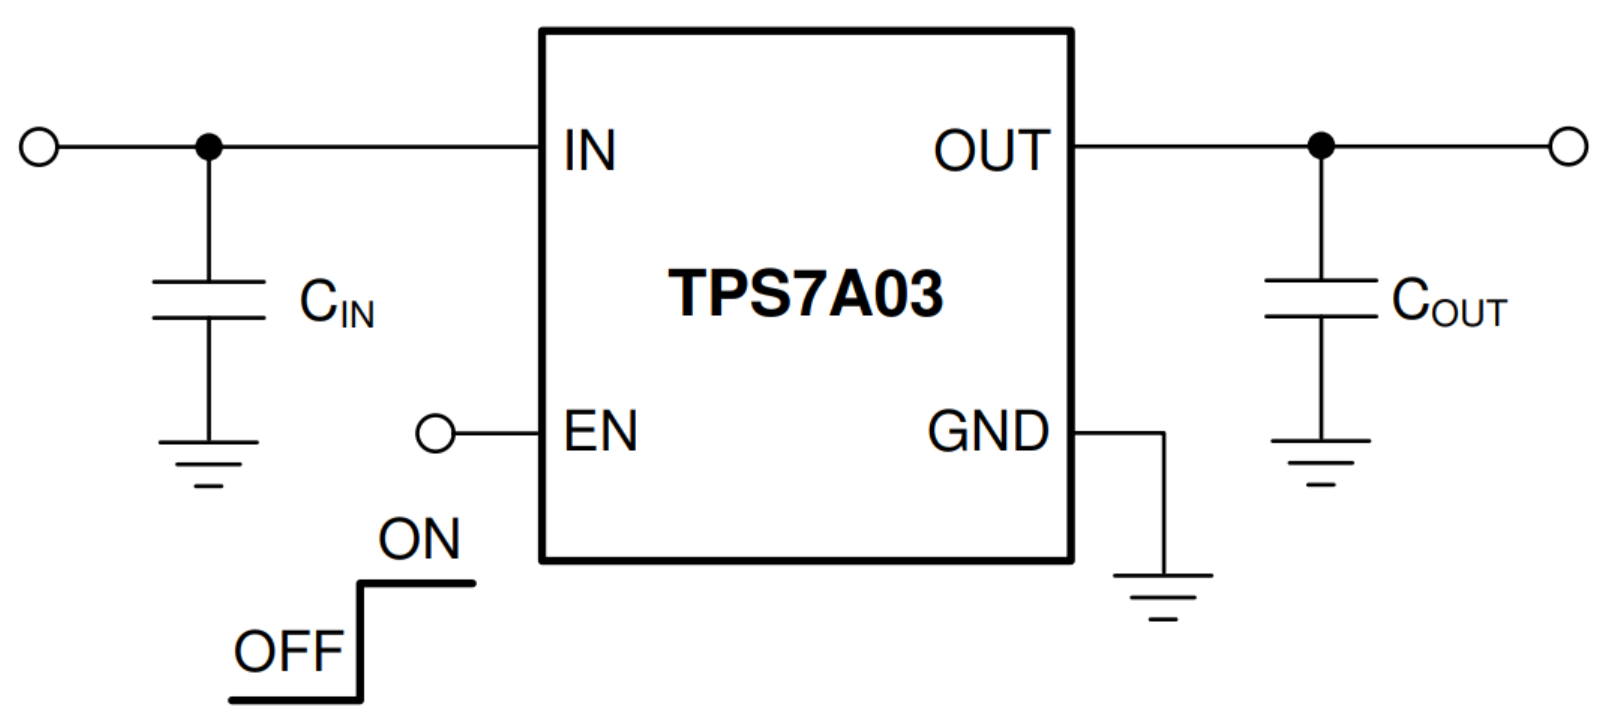
\includegraphics[width=0.6\textwidth]{Include/Figure/comp/tps7a03_typ_app.png}
	\caption{Typical application schematic - Source: \textit{TPS7A03}\cite{TPS7A03}}
	\label{fig:tps7a03_typ_app}
\end{figure}

\subsubsection{Absolute Maximum Ratings:}

The table \ref{tab:tps7a03_absolute_max_rating} shows the absolute maximum ratings provided by the datasheet of the \textit{TPS7A03}:

\begin{table}[H]
\centering
\begin{tabularx}{\textwidth}{|l|X|c|c|c|}
\hline
\textbf{ID} & \textbf{Description} & \textbf{MIN} & \textbf{MAX} & \textbf{UNIT} \\\hline
Voltage &  $V_{IN}$ & $-0.3 $ & $6.5$ & \si{\volt} \\\hline
Voltage &  $V_{EN}$ & $-0.3 $ & $6.5$ & \si{\volt} \\\hline
Voltage &  $V_{OUT}$ & $-0.3 $ & $V_{IN} + 0.3$ or $5.5$ & \si{\volt} \\\hline
Current & Max output & Inter. lim. & Internally limited & \si{\ampere} \\\hline
Temperature & Operating junction, $T_J$ & $-40$ & $150$ & \si{\celsius} \\\hline
Temperature & Stroage $T_{stg}$ & $-65$ & $150$ & \si{\celsius} \\\hline
\end{tabularx}
\caption{Absolute Maximum Ratings - Source: \textit{TPS7A03}\cite{TPS7A03}}
\label{tab:tps7a03_absolute_max_rating}
\end{table}

\subsubsection{Recommended Operating Conditions:}
The recommended operating conditions are given in table \ref{tab:tps7a03_recom_oper_cond}:

\begin{table}[H]
\centering
\begin{tabularx}{0.9\textwidth}{|l|X|c|c|c|c|}\hline
\textbf{ID} & \textit{Description} & \textbf{MIN} & \textbf{NOM} & \textbf{MAX} & \textbf{UNIT}\\\hline
$V_{IN}$ & Input voltage & $1.5$ & - & $6.0$ & \si{\volt}\\\hline
$V_{EN}$ & Enable voltage & $0$ & - & $6.0$ & \si{\volt}\\\hline
$V_{OUT}$ & Output voltage & $0.8$ & - & $5.0$ & \si{\volt}\\\hline
$I_{OUT}$ & Output current & $0$ & - & $200$ & \si{\milli\ampere}\\\hline
$C_{IN}$ & Input capacitor & - & $1$ & - & \si{\micro\farad}\\\hline
$C_{OUT}$ & Output capacitor & $1$ & $1$ & $22$ & \si{\micro\farad}\\\hline
$F_{EN}$ & \textit{EN} toggle frequency & - & - & $10$ & \si{\kilo\hertz}\\\hline
$T_J$ & Operating junction temperature & $-40$ & - & $125$ & \si{\celsius}\\\hline
\end{tabularx}
\caption{Recommended Operating Conditions - Source: \textit{TPS7A03}\cite{TPS7A03}}
\label{tab:tps7a03_recom_oper_cond}
\end{table}

\subsubsection{Design Recommendations:} \label{sec:ldo_reg_sel}
Figure \ref{fig:tps7a03_impl_schematic} illustrates a recommended implementation schematic for application power from a battery input supply:

\begin{figure}[H]
	\centering
	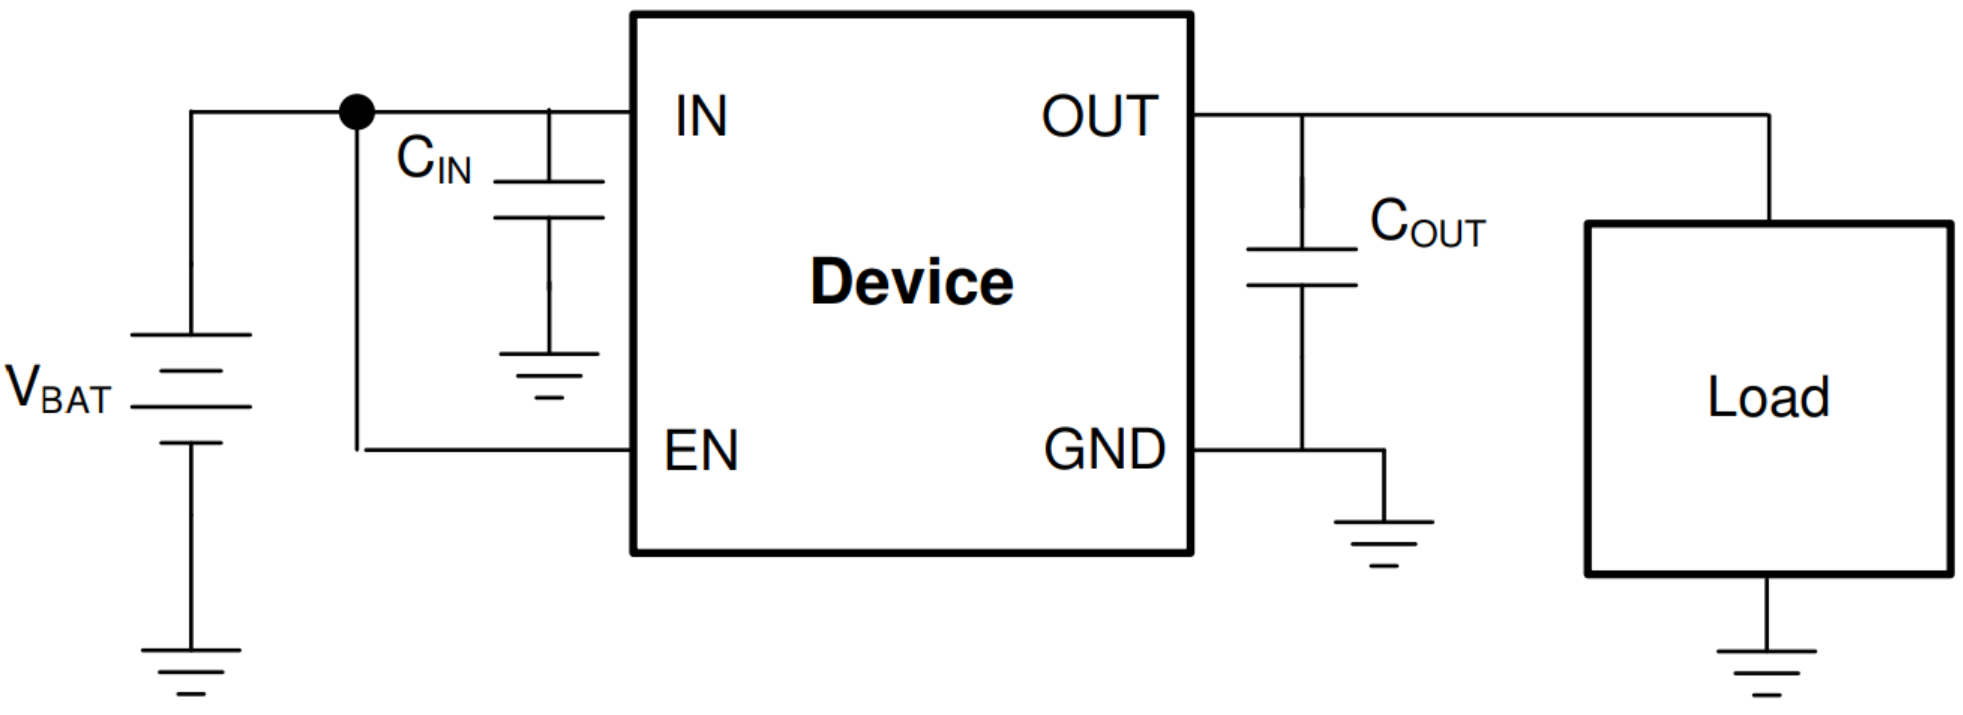
\includegraphics[width=0.7\textwidth]{Include/Figure/comp/tps7a03_recom_app.png}
	\caption{Recommended Implementation Schematic - Source: TPS7A03\cite{TPS7A03}}
	\label{fig:tps7a03_impl_schematic}
\end{figure}

\begin{enumerate}
\item \textbf{Input and output capacitors selection:}
\begin{itemize}[\;]
\item The implementation of the \textbf{TPS7A03} is straightforward and only require to add input and output ceramic capacitors: 
$$
\boxed{C_{IN} = \SI{1}{\micro\farad}} \quad \quad \quad \boxed{C_{OUT} = \SI{1}{\micro\farad}}
$$
\end{itemize}
\item \textbf{Temperature effect:}
\begin{itemize}[\;]
\item Temperature has a significant effect on the \textbf{TPS7A03} performances. Figure \ref{fig:tps7a03_temp_car} illustrate the current efficiency against the output current and the temperature:

\begin{figure}[H]
	\centering
	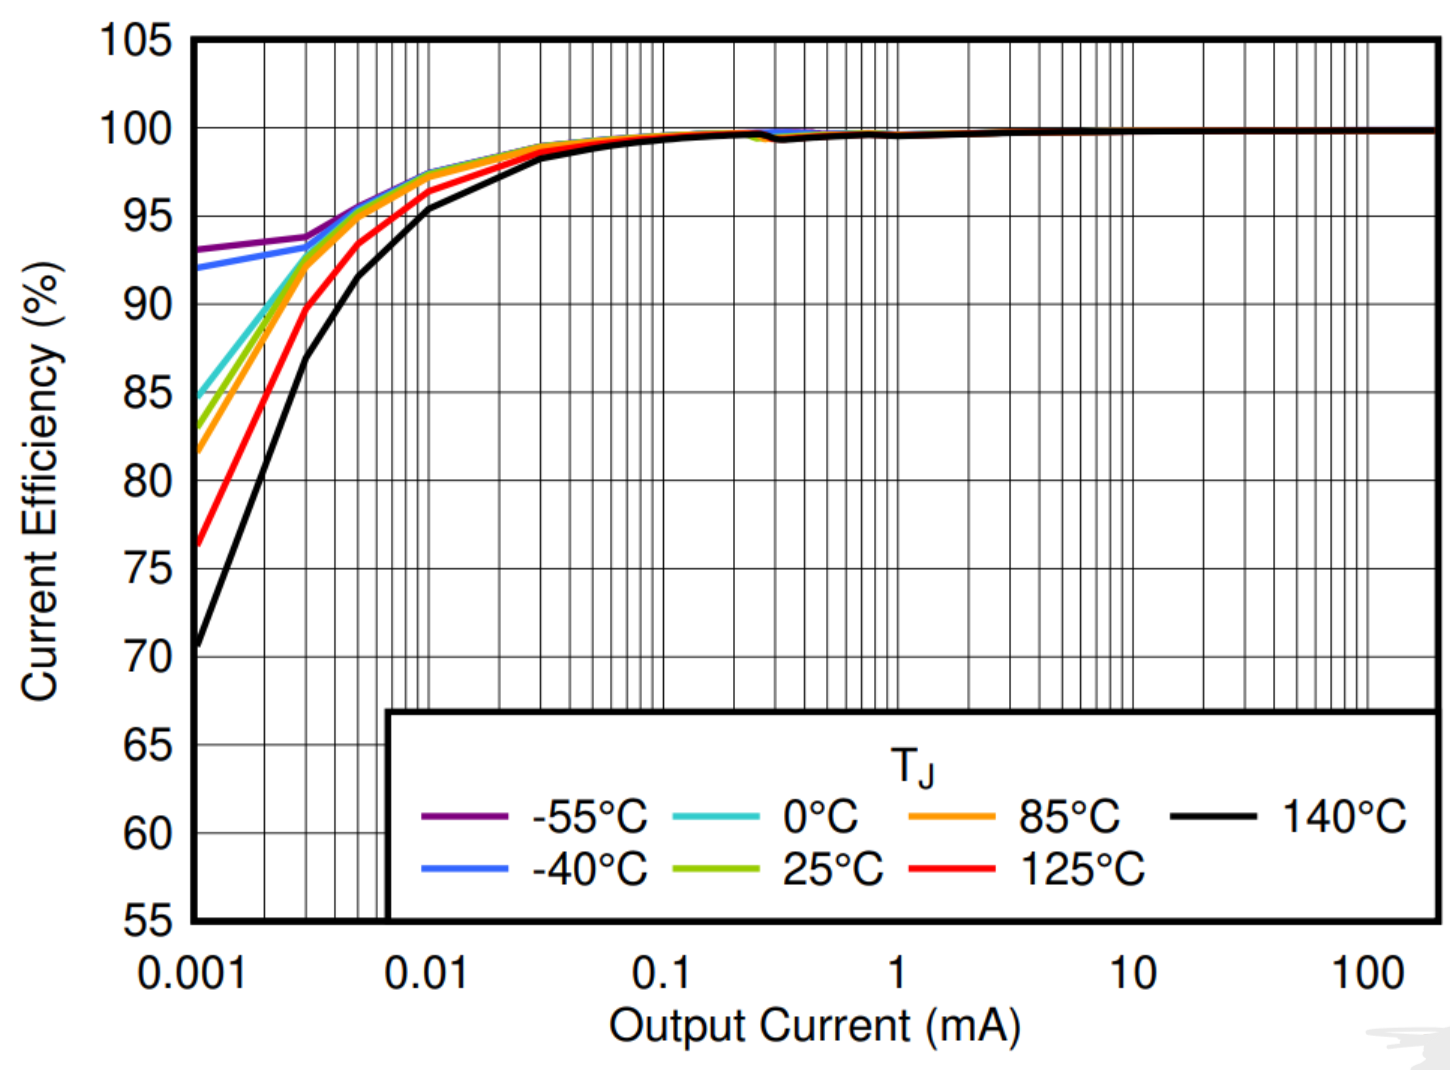
\includegraphics[width=0.6\textwidth]{Include/Figure/comp/tps7a03_temp_car.png}
	\caption{Current Efficiency vs $I_{OUT}$ and Temperature - Source: TPS7A03\cite{TPS7A03}}
	\label{fig:tps7a03_temp_car}
\end{figure}

\end{itemize}
\item \textbf{Power Supply Recommendations:}
\begin{itemize}
\item Power supply output voltage range of \SI{1.5}{\volt} to \SI{6.0}{\volt}
\item Power supply must regulated and free of spurious noise
\item To ensure good performances, $V_{IN}$ must be at least $V_{OUT(nom)} + \SI{0.5}{\volt}$
\end{itemize}
\end{enumerate}

%-------------------------------------------------------------------------------------
\subsection{WPC Receiver - BQ51013B}
Wireless charging became more and more usual in wearable device, therefore it was decided to include a wireless power receiver (\textit{WPC}) on the device.

\subsubsection{Description:}

The datasheet\cite{BQ51013B} describes the \textit{BQ51013B} as a single chip, advanced  and flexible secondary side for wireless power transfer up to \SI{5}{\watt} for portable applications. The chip provides a receiver with \textit{AC-to-DC} power conversion and regulation and fully integrates the digital control required to comply with the \textit{Wireless Power Consortium (WPC) Qi v1.2} communication protocol.\\

The \textit{BQ51013B} also integrates a low-resistance synchronous rectifier, a \textit{LDO}, digital control, and accurate voltage and current loops for a high efficiency and low power dissipation module.\\

 The \textit{BQ51013B} is design for portable applications, such as:
\begin{itemize}
\item \textit{WPC v1.2} compliant receivers
\item Cell phones and smart phones
\item Headsets
\item Digital cameras
\item Portable media players
\item Handheld devices
\end{itemize}

\subsubsection{Typical Application Diagram:}

Figure \ref{fig:bq51013b_simpl_schem} illustrates the simplified schematic of \textit{BQ51013B}:

\begin{figure}[H]
	\centering
	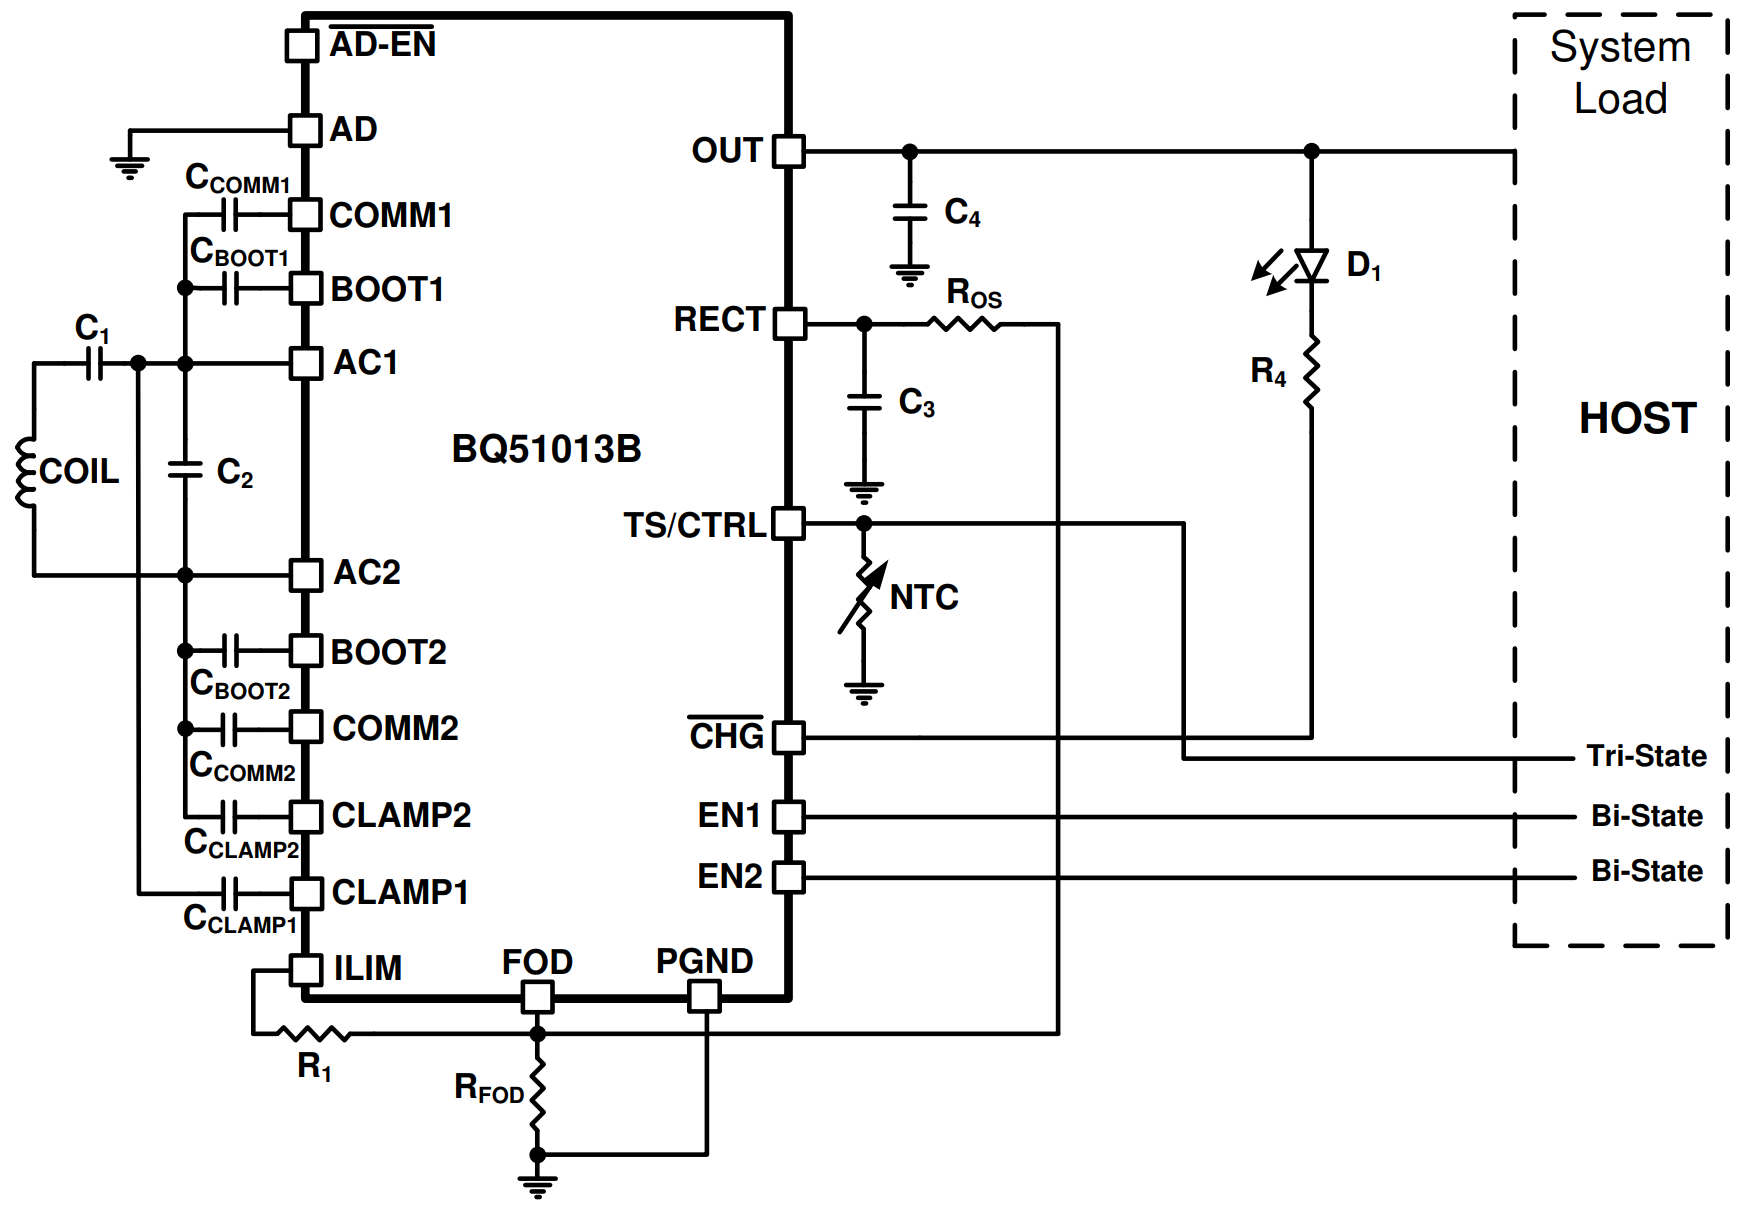
\includegraphics[width=0.75\textwidth]{Include/Figure/comp/bq51013b_simpl_schem.png}
	\caption{Simplified Schematic - Source: \textit{BQ51013B}\cite{BQ51013B}}
	\label{fig:bq51013b_simpl_schem}
\end{figure}

\subsubsection{Features:}

\begin{itemize}
\item \textbf{Specification and performances:}
\begin{itemize}
\item \SI{93}{\percent} Overall peak \textit{AC-DC} efficiency
\item \textit{WPC v1.2} compliant communication control
\item Output voltage conditioning
\item for Improved load transient response by dynamic rectifier control
\item Optimization of performance by dynamic efficiency scaling
\item Supports input up to \SI{20}{\volt}
\end{itemize}
\item \textbf{Control and safety features:}
\begin{itemize}
\item Rectifier over-voltage clamp with low-power dissipation ($V_{OVP} = \SI{15}{\volt}$)
\item Thermal shutdown protection
\item Control pin for temperature monitoring, charge complete, and fault host check 
\item Multifunction \textit{NTC} 
\end{itemize}
\item \textbf{Size and package:}
\begin{itemize}
\item VQFN 20-Pin : $\SI{4.5}{\milli\meter} \times \SI{3.5}{\milli\meter}$
\item DSBGA 28-Pin : $\SI{3.0}{\milli\meter} \times \SI{1.9}{\milli\meter}$
\end{itemize}
\end{itemize}

\subsubsection{Absolute Maximum Ratings:}

The table \ref{tab:bq51013b_absolute_max_rating} shows the absolute maximum ratings of the \textit{BQ51013B}:

\begin{table}[H]
\centering
\setlength{\extrarowheight}{2pt}
\begin{tabularx}{\textwidth}{|X|X|c|c|c|}
\hline
\textbf{ID} & \textbf{Description} & \textbf{MIN} & \textbf{MAX} & \textbf{UNIT} \\\hline
& AC1, AC2 & $-0.8$ & $20$ &  \\\cline{2-4}
& RECT, COMM1, COMM2, OUT, $\overline{\text{CHG}}$, CLAMP1, CLAMP2 & $-0.3$ & $20$ & \\\cline{2-4}
& AD, $\overline{\text{AD-EN}}$ & $-0.3$ & $30$ & \\\cline{2-4}
& BOOT1, BOOT2 & $-0.3$ & $26$ & \\\cline{2-4}
\multirow{-5}{*}[1em]{Input voltage}& EN1, EN2, FOD, TS/CTRL, ILIM & $-0.3$ & $7$ & \multirow{-5}{*}[1em]{\si{\volt}} \\\hline
Input current & AC1, AC2 & - & $2$ & \si{\ampere(RMS)} \\\hline
Output current & OUT & - & $1.5$ & \si{\ampere} \\\hline
\multirow{2}{*}{Output sink current} & $\overline{\text{CHG}}$ & - & $1500$ &  \multirow{2}{*}{\si{\ampere}}\\\cline{2-4}
 & COMM1, COMM2 & - & $1$ & \\\hline
Junction temperature & $T_{J}$ & $-40$ & $150$ & \si{\celsius} \\\hline
Storage temperature & $T_{stg}$ & $-65$ & $150$ & \si{\celsius} \\\hline
\end{tabularx}
\caption{Absolute maximum ratings - Source: \textit{BQ51013B}\cite{BQ51013B}}
\label{tab:bq51013b_absolute_max_rating}
\end{table}

\subsubsection{Recommended Operating Conditions:}

The table \ref{tab:bq51013b_recom_oper_cond} shows the recommended operation conditions of the \textit{BQ51013B}:

\begin{table}[H]
\centering
\begin{tabularx}{\textwidth}{|l|X|l|c|c|c|}\hline
\textbf{ID} & \textbf{Description} & \textbf{Pin} & \textbf{MIN} & \textbf{MAX} & \textbf{UNIT} \\\hline
$V_{RECT}$ & Voltage & RECT & $4$ & $10$ & \si{\volt} \\\hline
$I_{RECT}$ & Current through internal rectifier & RECT & - & $1.5$  & \si{\ampere} \\\hline
$I_{OUT}$ & Output current & OUT & - & $1.5$ & \si{\ampere} \\\hline
$V_{AD}$ & Adapter voltage & AD & & $15$ & \si{\volt} \\\hline
$I_{AD-EN}$ & Sink current & $\overline{\text{AD-EN}}$ & - & $1$ & \si{\milli\ampere} \\\hline
$I_{COMM}$ & COMMx sink current & COMM1, COMM2 & - & $500$ & \si{\milli\ampere} \\\hline
$T_J$ & Junction Temperature & \; & $0$ & $125$ & $\si{\celsius}$ \\\hline
\end{tabularx}
\caption{Recommended operating conditions - Source: \textit{BQ51013B}\cite{BQ51013B}}
\label{tab:bq51013b_recom_oper_cond}
\end{table}

\subsubsection{Design Recommendations:} \label{sec:wpc_rcvr_sel}
Concerning the implementation of the \textit{WPC} receiver, model chosen was the "\textit{Dual Power Path: Wireless Power and DC Input}" solution from the datasheet of the \textit{BQ51013B}\cite{BQ51013B} and the schematic of the \textit{bq51013xEVM-764} evaluation module (\textit{EVM}) from \textsc{Texas Instrument}.\\

Figure \ref{fig:bq51013b_impl_schem} illustrates "\textit{Dual Power Path: Wireless Power and DC Input}" solution schematic for the \textit{BQ51013B} wireless power receiver:

\begin{figure}[H]
	\centering
	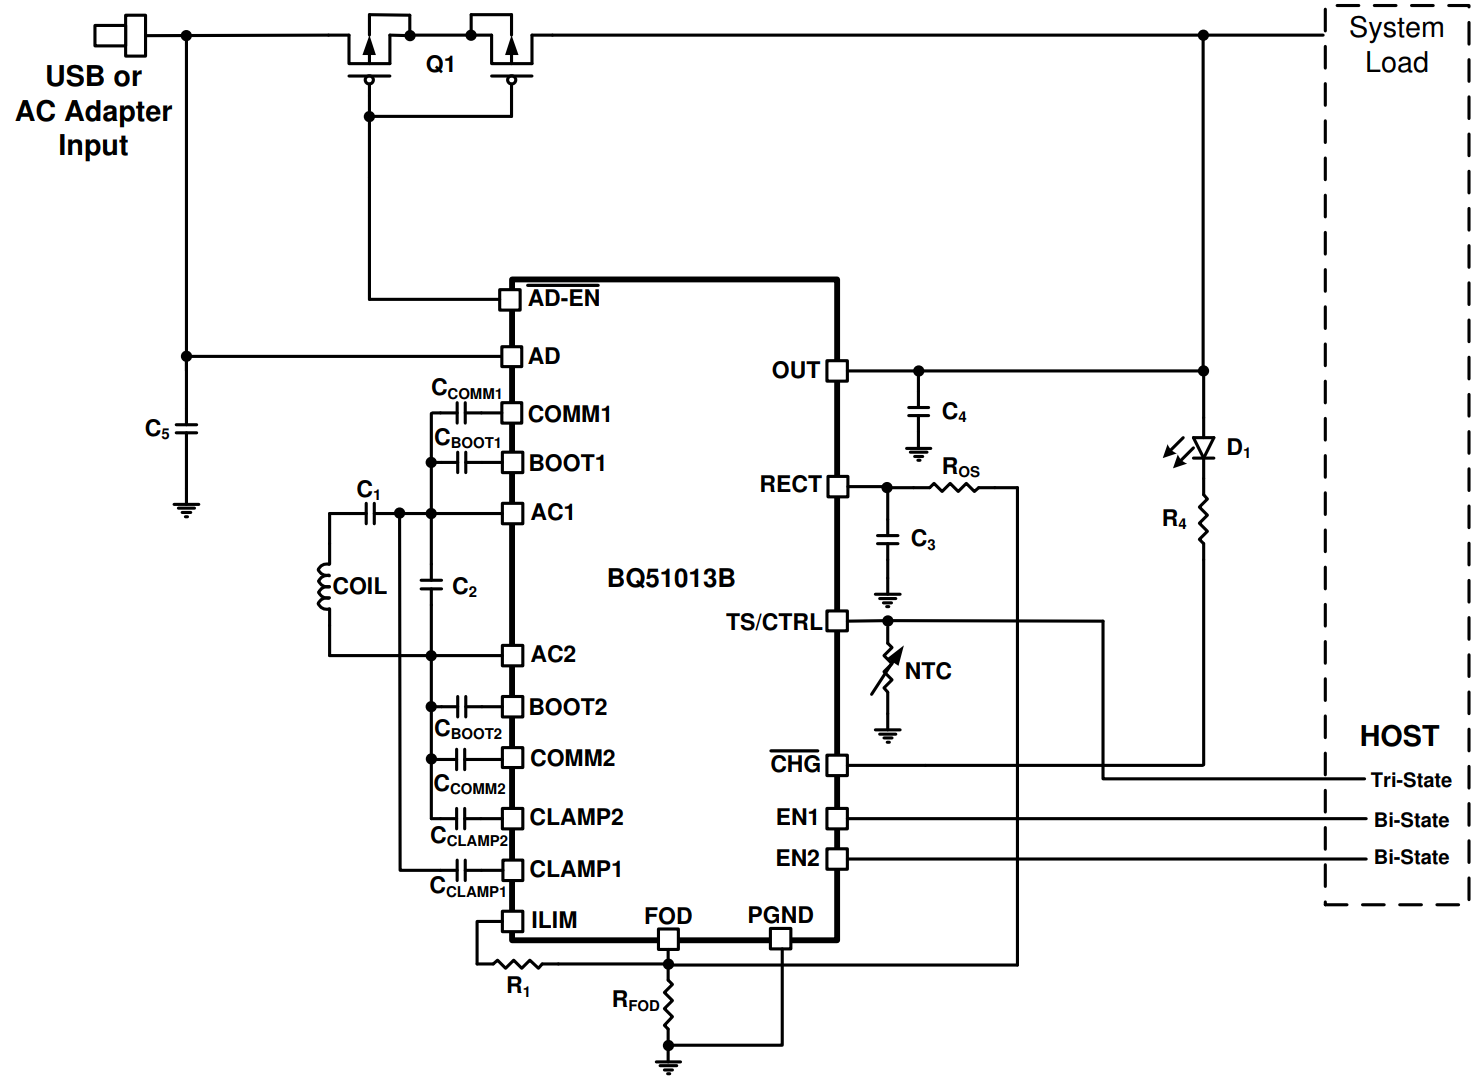
\includegraphics[width=0.8\textwidth]{Include/Figure/comp/bq51013b_impl_schem.png}
	\caption{Wireless Power Receiver and Power Supply for System Loads With Adapter Power-Path Multiplexing - Source: \textit{BQ51013B}\cite{BQ51013B}}
	\label{fig:bq51013b_impl_schem}
\end{figure}

\subsubsection{Series and Parallel Resonant Capacitor Selection}

Following the figure \ref{fig:bq51013b_res_cap_sel} from the datasheet of the \textit{BQ51013B}\cite{BQ51013B}, the series capacitors $C_1$ and parallel capacitors $C_2$ creates a dual resonant circuit with the receiver coil, therefore these two capacitors must be sized correctly according to the \textit{WPV v1.2} specification.

\begin{figure}[H]
	\centering
	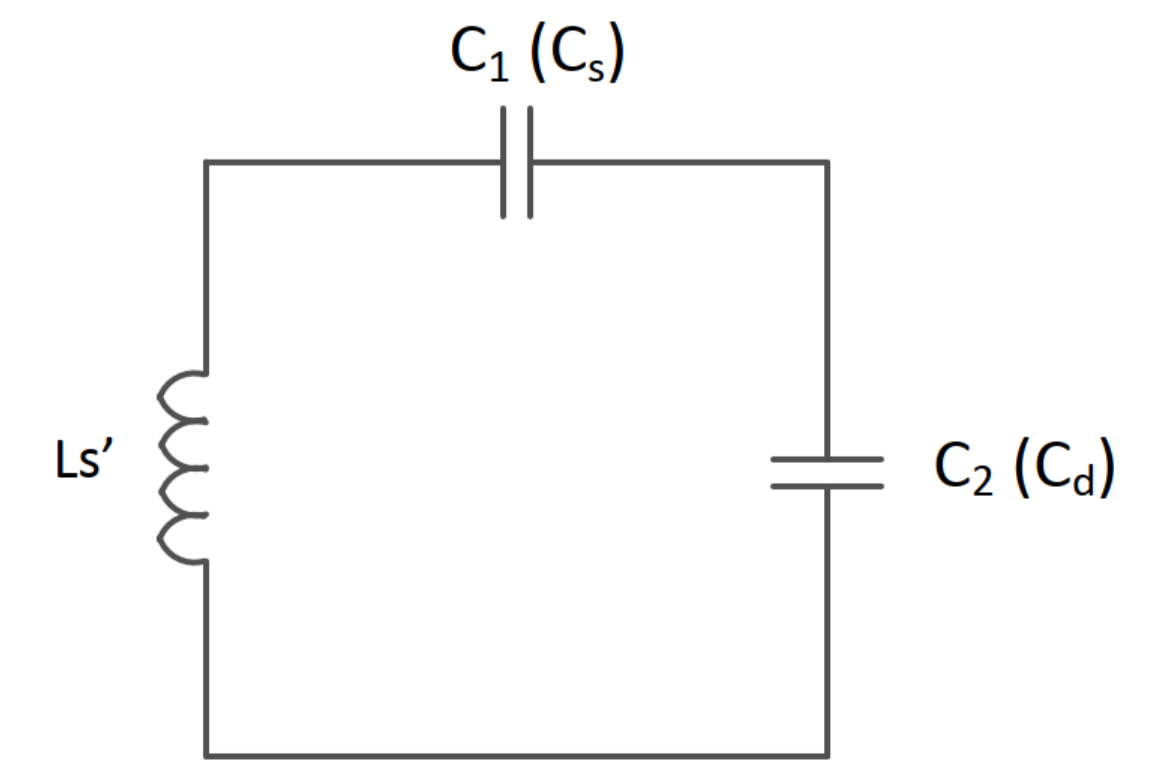
\includegraphics[width=0.35\textwidth]{Include/Figure/comp/bq51013b_res_cap_sel.png}
	\caption{Dual Resonant Circuit With the Receiver Coil - Source: \textit{BQ51013B}\cite{BQ51013B}}
	\label{fig:bq51013b_res_cap_sel}
\end{figure}

The two capacitors can be calculated with the equations \ref{eq:bq51013b_c1_c2}:
\begin{equation}
\label{eq:bq51013b_c1_c2}
\boxed{C_1 = \bigg[ \big(f_S \cdot 2 \pi\big)^2 \cdot L_S' \bigg]^{-1}} \quad \quad \quad
\boxed{C_2 = \bigg[ \big(f_D \cdot 2 \pi\big)^2 \cdot L_S - \dfrac{1}{C_1} \bigg]^{-1}} 
\end{equation}

Where:
$$
\begin{array}{l c r}
\ddl{f_S= \SI{100}{\kilo\hertz} +5/-10 \; \si{\percent}} & \quad \quad \quad & \ddl{f_D = \SI{1}{\mega\hertz} \pm \SI{10}{\percent}}
\end{array}
$$
\textbf{\underline{Note:}} $C_1$ must be chosen prior to calculating $C_2$.\\

According to the datasheet, the quality factor must be: \ddl{$Q>77$} and is determined with the equation \ref{eq:bq51013b_q}:

\begin{equation}
\label{eq:bq51013b_q}
\boxed{Q = \dfrac{2 \pi \cdot f_D \cdot L_S}{R}}\quad \quad \quad \text{Where, } R:\text{DC resistance of the receiver coil}
\end{equation}

Following the solution from the datasheet, the selected inductance for the application gives:
$$
\ddl{L_S = \SI{11}{\micro\henry}} \quad\quad\quad \ddl{L_S' = \SI{16}{\micro\henry}} \quad\quad\quad \ddl{R = \SI{191}{\milli\ohm}}
$$

Using the equation \ref{eq:bq51013b_c1_c2}:
$$
C_1 = \bigg[ \big( 100\cdot 10^3 \cdot 2\pi \big)^2 \cdot 16\cdot 10^{-6} \bigg]^{-1} = \ddl{\SI{158.3}{\nano\farad}}
$$

With $f_S$ $(+5/-10\si{\percent})$, the range of $C_1$ is: $\ddl{\SI{144}{\nano\farad}\leq C_1 \leq \SI{175}{\nano\farad}}$\\

For an optimal solution of three parallel capacitors, the selected values are:
$$
\boxed{
\begin{array}{c}
C_{1a} = \SI{68}{\nano\farad}, \; C_{1b} = \SI{47}{\nano\farad}, \; C_{1c} = \SI{39}{\nano\farad} \quad \Rightarrow \quad C_{1tot} = \ddl{\SI{154}{\nano\farad}}
\end{array}}
$$

With $C_1$ defined, it is possible to calculate $C_2$ (eq. \ref{eq:bq51013b_c1_c2}):

$$
C_2 = \bigg[ \big( 1\cdot 10^6 \cdot 2\pi \big)^2 \cdot 11\cdot 10^{-6} - \dfrac{1}{154\cdot 10^{-9}} \bigg]^{-1} = \ddl{\SI{2.3}{\nano\farad}}
$$

An easy solution of two capacitors is:
$$
\boxed{C_{2a} = \SI{2.2}{\nano\farad}, \; C_{2b} = \SI{100}{\pico\farad} \quad \Rightarrow \quad C_{2tot} = \ddl{\SI{2.3}{\nano\farad}}}
$$

Now, the quality factor condition can be tested (eq. \ref{eq:bq51013b_q}):
$$
	Q = \dfrac{2\pi \cdot 10^6 \cdot 11\cdot 10^{-6}}{191\cdot 10^{-3}} = \ddl{361.86 > 77} \; \textcolor{mygreen}{\Large \checkmark}
$$

Those values of capacitors are totally dependent to the used coil and must be adapted to the used coil specification. The datasheet also recommend to use ceramic capacitors with a \textbf{minimum voltage range} of \ddl{\SI{25}{\volt}}.

\subsubsection{COMM, CLAMP, and BOOT Capacitors Selection}

COMM, CLAMP and BOOT capacitors values from the \textit{BQ51013BEVM-764} evaluation module of the \textit{BQ51013B} can be used for most application:
$$
\boxed{\begin{array}{l c l c l}
C_{BOOT1} & = & C_{BOOT2} & = & \ddl{\SI{10}{\nano\farad}} \\
C_{CLAMP1} & = & C_{CLAMP2} & = & \ddl{\SI{470}{\nano\farad}} \\
C_{COMM1} & = & C_{COMM2} & = & \ddl{\SI{22}{\nano\farad}}
\end{array}}
$$

\textbf{\underline{Note:}} All capacitors must have a \textbf{minimum voltage range} of \ddl{\SI{25}{\volt}}.

\subsubsection{Control Pins and $\overline{\textbf{CHG}}$ external components selection}
The \textbf{TS/CTRL} pin can be used as a temperature sensor with an external \textit{NTC} of \SI{10}{\kilo\ohm}. Even with a \textit{NTC} connected, this pin can still be used as system controller. In this case de \textit{GPIO} will be in high impedance for normal temperature sense control.\\

The $\overline{\textbf{CHG}}$ can be used as a power transfer indicator by connecting a forward bias LED and a current limiting series resistor.

\subsubsection{Current Limit and FOD External Components Selection}

The \textit{BQ51013B} also have a current limit and foreign object (\textit{FOD}) functions. Those two functions are related:
\begin{itemize}
\item $R_1 + R_{FOD}$ set the current limit
\item \textit{FOD} calibration determines $R_{FOD}$ and $R_{OS}$, default value:
$$
	\boxed{R_{FOD} = \SI{196}{\kilo\ohm}} \quad \quad \quad \boxed{R_{OS} = \SI{20}{\kilo\ohm}}
$$
\end{itemize}

The equations \ref{eq:bq51013b_rilim} are used to determine the value of $R_1$ and $R_{FOD}$:
\begin{equation}
\label{eq:bq51013b_rilim}
\boxed{\begin{array}{l l}
R_{ILIM} = \dfrac{K_{IMAX}}{I_{MAX}} & R_{ILIM} = R_1 + R_{FOD}\\
I_{ILIM} = 1.2 \cdot I_{MAX} = \dfrac{K_{ILIM}}{R_{ILIM}}
\end{array}}
\end{equation}

Where:

\begin{itemize}
\item $I_{MAX}$ : Expected maximum output current during normal operation
\item $I_{ILIM}$ : Hardware over-current limit
\end{itemize}

For the \textit{LTEWatch} device:
$$
I_{MAX} = \SI{1}{\ampere} \quad \quad R_{FOD} = \SI{196}{\ohm} \quad
K_{IMAX} = \SI{262}{\ampere\ohm} \quad \quad K_{ILIM} = \SI{314}{\ampere\ohm} 
$$

The resistance $R_1$ can be determined with equations \ref{eq:bq51013b_rilim}:
$$
\begin{array}{c}
	I_{ILIM} = 1.2 \cdot I_{MAX} = 1.2 \cdot 1 = \ddl{\SI{1.2}{\ampere}} \;\rightarrow \; R_{ILIM} = \dfrac{K_{ILIM}}{I_{ILIM}} = \dfrac{314}{1.2} = \ddl{\SI{262}{\ohm}}\\[12pt]
	\boxed{\Rightarrow \; R_1 = R_{ILIM}-R_{FOD} = \ddl{\SI{66}{\ohm}}}
\end{array}
$$

\subsubsection{RECT and OUT Capacitance Selection}

A capacitor is connected to RECT to smooth th \textit{AC-to-DC} conversion and prevent minor current transient from passing to OUT. The datasheet recommends to use two $\SI{10}{\micro\farad}$ capacitors followed by one $\SI{100}{\nano\farad}$ for $I_{MAX} = \SI{1}{\ampere}$. The capacitors must be rated to at least $\SI{16}{\volt}$.

A capacitor connected on OUT is used to smooth any ripple from minor load transients. A single $\SI{10}{\micro\farad}$ capacitors followed by a single $\SI{100}{\nano\farad}$ is enough.

\subsubsection{Dual Power Path Blocking FET Selection}

In dual power path solution, an external blocking FET is required. The datasheet of the \textit{BQ51013B} recommends the \textit{CSD75207W15}, which is \textit{WCSP} package integrated a \textit{P-Channel}, \SI{20}{\volt}, \SI{3.9}{\ampere} FET pair.\\

As the \textit{CSD75207W15} component was not available, another model with similar specification was used. The selected component is the \textit{CSD75208W1015}, a \textit{P-Channel}, \SI{20}{\volt}, \SI{1.6}{\ampere} FET pair, which is enough for the \textit{LTEWatch} application.

\subsubsection{EN1 and EN2 Inputs}

EN1 and EN2 are used to enable/disable the wireless/wired charging (tab. \ref{tab:bq51013b_en1_en2}):

\begin{table}[H]
\centering
\begin{tabular}{|c|c|l|}\hline
\textbf{EN1} & \textbf{EN2} & \textbf{Description}\\\hline
0 & 0 & Wireless charging is enabled\\\hline
0 & 1 & Dynamic communication current limit disabled\\\hline
1 & 0 & Wireless charging disabled\\\hline
1 & 1 & Wireless charging disabled\\\hline
\end{tabular}
\caption{Recommended operating conditions - Source: \textit{BQ51013B}\cite{BQ51013B}}
\label{tab:bq51013b_en1_en2}
\end{table}


%-------------------------------------------------------------------------------------

\subsection{Accelerometer - MC3635}
\begin{figure}[H]
	\centering
	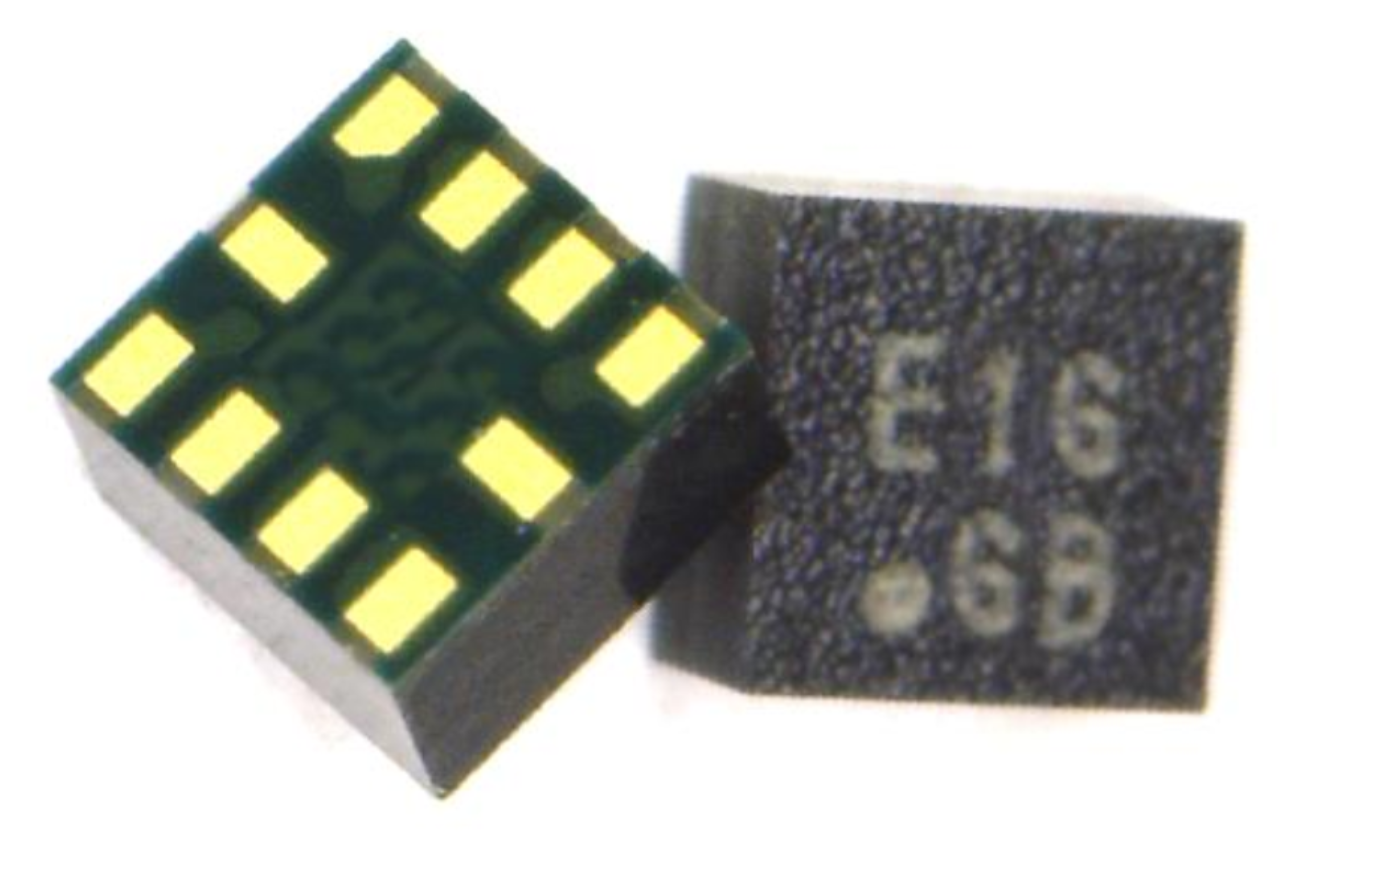
\includegraphics[width=0.4\textwidth]{Include/Figure/comp/MC3635_picti.png}
	\caption{MC3635 3-Axis Accelerometer from \textsc{mCube} - Source: \textit{MC3635}\cite{MC3635}}
	\label{fig:MC3635_picti}
\end{figure}

\subsubsection{Description:}

The \textit{MC3635}\cite{MC3635} is described in its datasheet as an ultra-low power, low-noise, integrated digital output 3-axis accelerometer optimized for wearable applications and \textit{IoT} devices.

\subsubsection{Features:}

\begin{itemize}
\item \textbf{Range, Sampling and Power:}
\begin{itemize}
\item $\pm$2, 4, 8, 12 or \SI{16}{\g} ranges
\item 8, 10 or \SI{12}{\bit} resolution with \textit{FIFO} or \SI{14}{\bit} single samples
\item Sample rate from $14$ to \SI{1300}{sample\per\second} that can be triggered via:
\begin{itemize}
\item Internal oscillator
\item Clock pin
\item Software command
\end{itemize}
\item \textit{Sniff} and \textit{Wake} modes:
\begin{itemize}
\item \SI{0.4}{\micro\ampere} \textit{Sniff} current at \SI{6}{\hertz}
\item Separate or combined \textit{Sniff}/\textit{Wake}
\end{itemize}
\item Ultra-Low Power with \SI{32}{sample} \textit{FIFO}:
\begin{itemize}
\item \SI{0.9}{\micro\ampere} typical current at \SI{25}{\hertz}
\item \SI{1.6}{\micro\ampere} typical current at \SI{50}{\hertz}
\item \SI{2.8}{\micro\ampere} typical current at \SI{100}{\hertz}
\item \SI{36}{\micro\ampere} typical current at \SI{1.3}{\kilo\hertz}
\end{itemize}
\end{itemize}
\item \textbf{System Integration:}
\begin{itemize}
\item \textit{I2C} interface up to \SI{1}{\mega\hertz}
\item \textit{SPI} Interface up to \SI{4}{\mega\hertz}
\item $1.6 \times 1.6 \times \SI{0.94}{\milli\meter}$ 10 Pin package
\item Single-chip \textit{3D silicon MEMS}
\item Low noise to \SI{2.3}{\milli\g (RMS)}
\end{itemize}
\end{itemize}

\pagebreak

\subsubsection{Typical Application Diagram:}\label{sec:accl_sel}

Figure \ref{fig:MC3635_typ_app_4spi} illustrates a typical 4-wire \textit{SPI} Application Circuit for the \textit{MC3635}:

\begin{figure}[H]
	\centering
	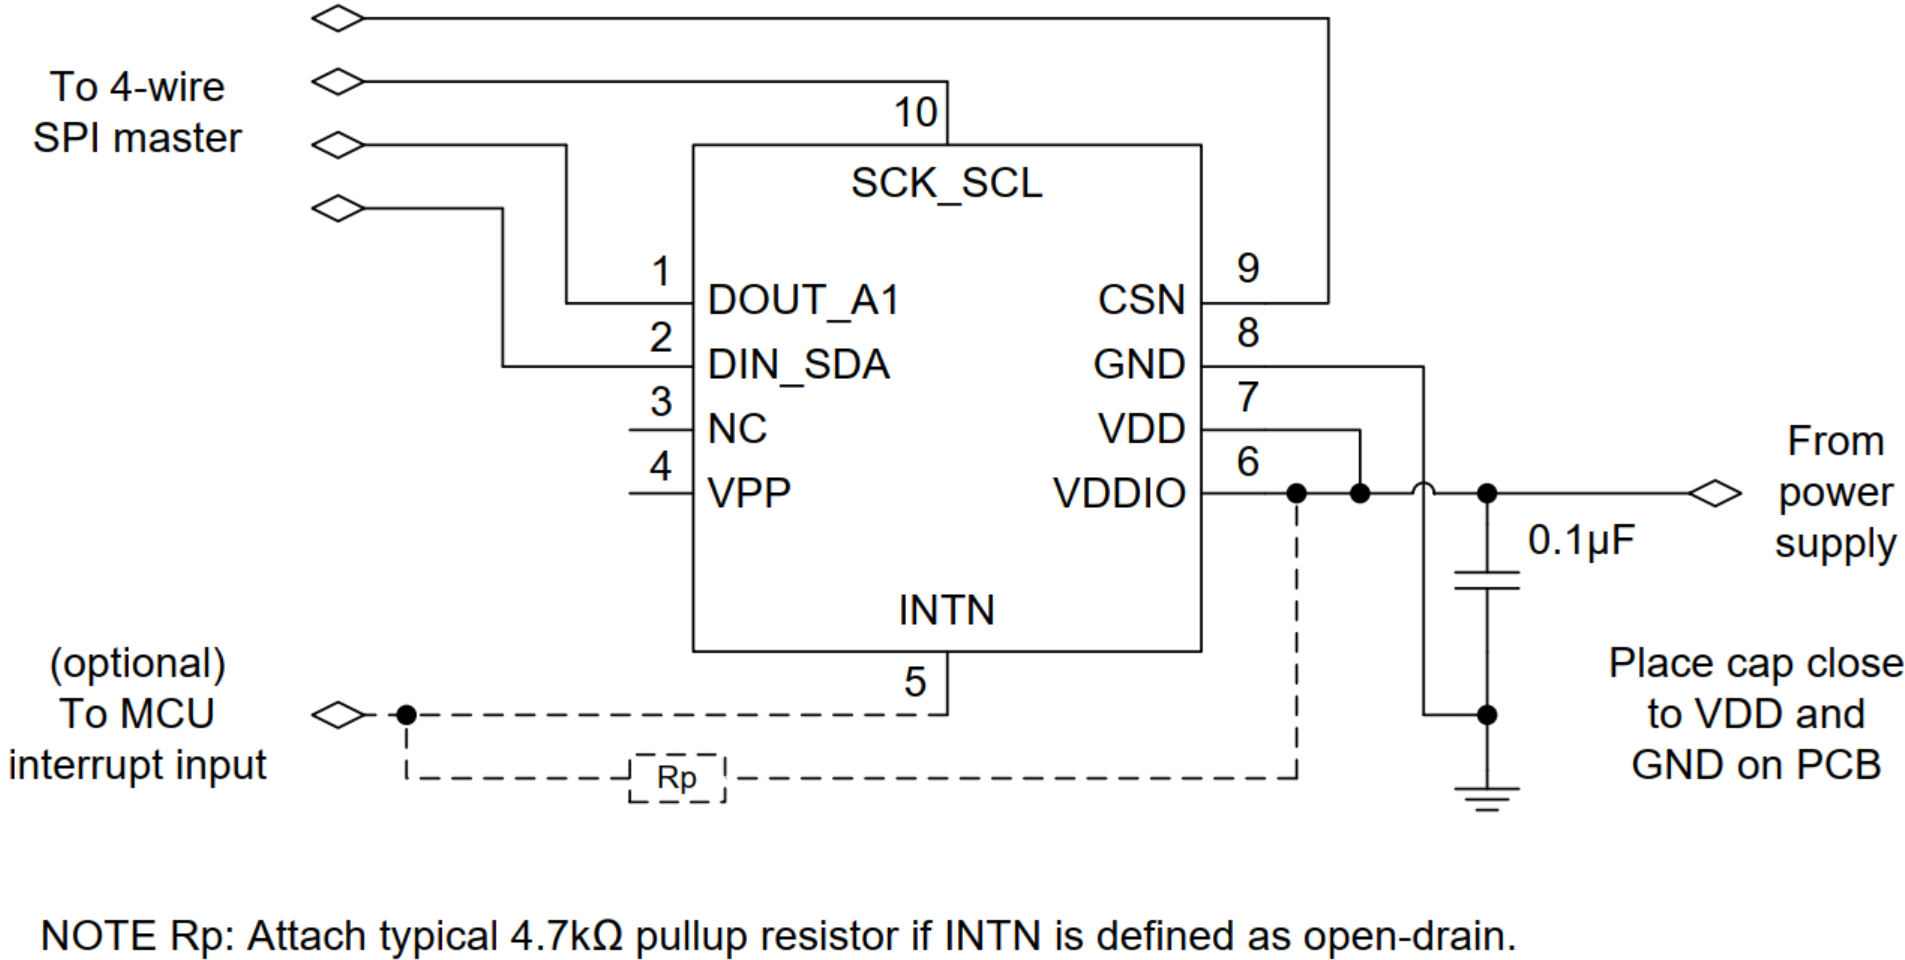
\includegraphics[width=1\textwidth]{Include/Figure/comp/MC3635_typ_app_4spi.png}
	\caption{Typical 4-wire SPI Application Circuit - Source: \textit{MC3635}\cite{MC3635}}
	\label{fig:MC3635_typ_app_4spi}
\end{figure}


\subsubsection{Absolute Maximum Ratings:}

The table \ref{tab:MC3635_absolute_max_rating} shows the absolute maximum ratings provided by the datasheet of the \textit{MC3635}:

\begin{table}[H]
\centering
\begin{tabularx}{\textwidth}{|X|X|c|c|c|}
\hline
\textbf{ID} & \textbf{Symbol} & \textbf{MIN} & \textbf{MAX} & \textbf{UNIT} \\\hline
Supply Voltages & VDD, VDDIO & $-0.3$ & $+3.6$ & \si{\volt} \\\hline
Acceleration, any axis, \SI{100}{\micro\second} & $g_{MAX}$ & - & 10000 & g \\\hline
Ambient operating temperature & $T_{OP}$ & $-40$ & $+85$ & \si{\celsius} \\\hline
Storage temperature & $T_{STG}$ & $-40$ & $+125$ & \si{\celsius} \\\hline
ESD human body model & \textit{HBM} & $-2$ & $+2$ & \si{\kilo\volt} \\\hline
Input voltage to non-power pin & CSN, DIN\_SDA, DOUT\_A1, INTN, SCK\_SCL & $-0.3$ & (VDDIO $+ 0.3$) or $3.6$ & \si{\volt} \\\hline
\end{tabularx}
\caption{Absolute Maximum Ratings - Source: \textit{MC3635}\cite{MC3635}}
\label{tab:MC3635_absolute_max_rating}
\end{table}

%-------------------------------------------------------------------------------------
\pagebreak
\subsection{LCD Display - LS011B7DH03} \label{sec:disp_sel}
Even if the \textit{LTEWatch} use clock hands to display the time, it is also a connected smart-watch which means that the device require à screen to display more complex information, such as date, connection state, notifications and settings.\\

Finding a display for the \textit{LTEWatch} is not an easy task despise the fact that smart-watch round format display are widely available. The perfect solution would be a perforated round display to let the clock hands rotor pass through the screen. This kind require custom order and are not available for average customer and require too much time to be a suitable solution for this Master Thesis project. The best compromise solution for the moment is to select a display that is small enough to be placed next to the motors on a 45-\SI{50}{\milli\meter} diameter watch.\\

The next step is to choose the display technology. After many research the selected display is the \textit{LS011B7DH03}\cite{LS011B7DH03} from \textsc{Sharp} which is a \textit{Memory In Pixel (MIP)} \textit{LCD}, a display technology specifically design for outdoor application with battery supply. 

\begin{figure}[H]
\begin{subfigure}{.6\textwidth}
	\centering
	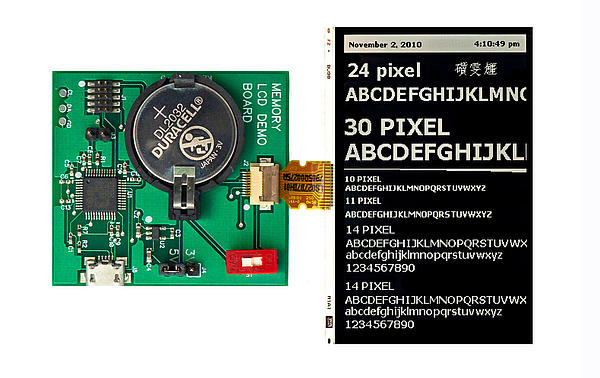
\includegraphics[width=1\textwidth]{Include/Figure/comp/csm_Sharp-MIP-3-16-inch-Edit_b0c527d887.jpg}
	\end{subfigure}
\begin{subfigure}{.4\textwidth}
	\centering
	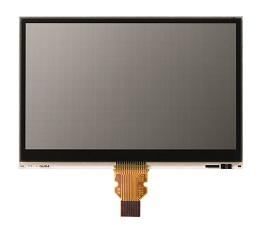
\includegraphics[width=1\textwidth]{Include/Figure/comp/Sharp-Product-Memory-in-Pixel-LCD-Displays_smaller.jpg}
	\end{subfigure}
	\caption{\textsc{Sharp} \textit{MIP} Display Technology - Source:\cite{SHARPMIP}}
	\label{fig:Sharp_mip_1}
\end{figure}


\subsubsection{Description:}


On \textsc{Sharp} website\cite{SHARPMIP}, their \textit{MIP} LCDs are described as, ultra-low power consumption and high readability screen for any ambient lighting ans environment. They exist in 64 colors or high-contrast monochrome solution.\\

\textit{MIP} screen are reflective screen, this mean that they do not require back light which can already drastically reduce the consumption of the device. The display driver circuits is also directly integrated into the panel for a easy to implement, lightweight and compact solution.\\

\pagebreak
\begin{flushleft}
\textsc{Sharp} Memory-in-Pixel LCDs offer the following features:
\end{flushleft}
\begin{itemize}
\item \textbf{Product Line-up:}
\begin{itemize}
\item Available in diagonal sizes ranging from \SI{1.08}{"} to \SI{4.40}{"} (\SI{27,432}{\milli\meter} to \SI{111.785}{\milli\meter})
\end{itemize}
\item \textbf{High readability:}
\begin{itemize}
\item Viewable in any light, from edge-of-vision to bright sunlight.
\end{itemize}
\item \textbf{Color solutions:}
Available in 64 colors or Monochrome solution
\item \textbf{Operating Temperature:}
\begin{itemize}
\item Wide operating temperatures for the most extreme environments
\end{itemize}
\item \textbf{View Angle:}
\begin{itemize}
\item Wide, symmetrical viewing angles, typically $\SI{120}{\degres}\times \SI{120}{\degres}$
\end{itemize}
\item \textbf{Ultra-low Power Consumption:}
\begin{itemize}
\item Consumption of only \SI{1.25}{\percent} to \SI{2.5}{\percent} of a \textit{STN} LCD’s and approximately \SI{0.1}{\percent} of an \textit{AM-TFT} LCD’s
\item Excellent reflective display performance without the need for a backlight
\item TFT glass with monolithic embedded driver and peripheral circuits. Each pixel contains \SI{1}{\bit} \textit{SRAM} memory to stores graphic data, therefore still image does not require continuous refresh. Moreover, refresh require less power than with traditional graphic displays:
\begin{table}[H]
\centering
\begin{tabular}{|l|c|c|}\hline
\textbf{Model} & $128 \times 128$ & $400 \times 240$\\\hline
\textbf{Static Image} & \SI{12}{\micro\watt} & \SI{50}{\micro\watt} \\\hline
\textbf{\SI{1}{\hertz} Dynamic Update }& \SI{50}{\micro\watt} & \SI{175}{\micro\watt} \\\hline
\end{tabular}
\caption{Power Consumption for \SI{1.28}{"} and \SI{2.7}{"} Memory \textit{LCDs}}
\label{tab:sharp_mip_pwr}
\end{table}
\end{itemize}
\item \textbf{Interface:}
\begin{itemize}
\item Easy implementation with a 3 wires \textit{SPI} serial interface (\textit{SI}, \textit{SCS}, \textit{SCK})
\end{itemize}
\item \textbf{Fast Image Refresh Time:}
\begin{itemize}
\item \textit{MIP LCDs} have fast response times for scrolling text and moving images, way better performances than \textit{Cholesteric}, \textit{STN}, and \textit{E-Ink} displays.
\begin{table}[H]
\centering
\begin{tabular}{|l|c|}\hline
\centered{\textbf{Data Refresh Rate}} & \SI{20}{\hertz} (typ.) \\\hline
\centered{\textbf{\textit{LCD} Response time} \\ (Black to White/White to Black} & \SI{10}{\micro\second}/\SI{20}{\micro\second} \\\hline
\end{tabular}
\caption{Refresh Rate and Time Performances Of Memory \textit{LCDs}}
\label{tab:sharp_mip_rfrsh}
\end{table}
\end{itemize}
\end{itemize}

Memory-in-Pixel (\textit{MIP}) LCDs from \textsc{Sharp} seems to be a suitable solution for \textit{LTEWatch}. Based on this choice, the best fitting model is the \textit{LS011B7DH03}. The following sections are based on the datasheet of the \textit{LS011B7DH03}\cite{LS011B7DH03}.

\subsubsection{Features:}

The \textit{LS011B7DH03} \textit{MIP} \textit{LCD} from \textsc{Sharp} have the following features: 

\begin{itemize}
\item \textbf{Performances and Image Quality:}
\begin{itemize}
\item Reflective \textit{TFT-LCD} active-matrix with slightly transmissive panel of white and black
\item Screen with \SI{1.08}{"} diagonal and $160 \times 68$ resolution for a total strip array of \SI{10880}{pixels}
\item Screen with an anti-glare \textit{AG} front polarized surface
\item High image refresh rate range up to \SI{70}{\hertz}
\end{itemize}
\item \textbf{Controls and Interfaces}:
\begin{itemize}
\item Mounted with a 10-Pin flat cable compatible with \textit{FPC} type connector
\item Simple 3-wire \textit{SPI} serial data signal communication up to \SI{1}{\mega\hertz}
\item Panel with integrated data storage of \SI{1}{\bit} per pixel
\item Arbitrary line data renewable mode
\end{itemize}
\item \textbf{Mechanical Properties:}
\begin{itemize}[\quad\;\;]
\item Monolithic construction for a compact, thin and lightweight panel with an outline dimension of \SI{32}{\milli\meter}$\times$\SI{14}{\milli\meter}$\times$\SI{0.745}{\milli\meter} (W$\times$H$\times$D)
\end{itemize}
\item \textbf{Power Consumption}
\begin{enumerate}
\item Hold Mode (no display data update with all black pattern):
\begin{enumerate}[a)]
\item \SI{15}{\micro\watt} (typ.)
\item \SI{50}{\micro\watt} (max)
\end{enumerate}
\item Data update mode (\SI{1}{\hertz} with vertical stripe pattern):
\begin{enumerate}[a)]
\item \SI{25}{\micro\watt} (typ.)
\item \SI{100}{\micro\watt} (max)
\end{enumerate}
\end{enumerate}
\end{itemize}

\subsubsection{Mechanical Specification}

Mechanical specification of the \textit{LS011B7DH03} is presented in table \ref{tab:LS011B7DH03_mech_spec}

\begin{table}[H]
\centering
\begin{tabular}{|l|l|c|}\hline
\textbf{ID} & \textbf{Specification} & \textbf{Unit}\\\hline
Screen size & \SI{1.8}{"} & inch\\\hline
Active area (H$\times$V)& $25.28 \times 10.744$ & \si{\milli\meter}\\\hline
Dot configuration (H$\times$V) & $160 \times 68$ & Dot (Pixel)\\\hline
Pixel array & square & -\\\hline
Display mode & Normally White & -\\\hline
Outline dimension (W$\times$H$\times$D) & $32.000 \times 14.000 \times 0.745$ & \si{\milli\meter}\\\hline
Mass (max) & $0.73$ & \si{\gram}\\\hline
Surface hardness & $3\text{H}$ & Pencil Hardness \\\hline
Surface treatment & Anti-Glare (\textit{AG}) & - \\\hline
\end{tabular}
\caption{Mechanical specification of the \textit{LS011B7DH03} - Source: datasheet\cite{LS011B7DH03}}
\label{tab:LS011B7DH03_mech_spec}
\end{table}

\subsubsection{Absolute Maximum Ratings:}

Absolute maximum ratings of the \textit{LS011B7DH03} are presented in table \ref{tab:LS011B7DH03_absolute_max_rating}:

\begin{table}[H]
\centering
\begin{tabular}{|l|c|c|c|c|}\hline
\textbf{ID} & \textbf{Symbol} & \textbf{MIN} & \textbf{MAX} & \textbf{Unit}\\\hline
\multirow{2}{*}{Power Supply Voltage} & VDDA & $-0.3$ & $+3.6$ & \si{\volt}\\\cline{2-5}
										& VDD & $-0.3$ & $+3.6$ & \si{\volt}\\\hline
Input Signal Voltage (\textit{Hi}) & VHI & - & VDD & \si{\volt}\\\hline
Input Signal Voltage (\textit{Low}) & VLI & $-0.3$ & VDD & \si{\volt}\\\hline
Storage Temperature & $T_{stg}$ & $-30$ & $+80$ & \si{\celsius}\\\hline
Operating Temperature & $T_{opr}$ & $-20$ & $+70$ & \si{\celsius}\\\hline
\end{tabular}
\caption{Absolute Maximum Ratings - Source: \textit{LS011B7DH03}\cite{LS011B7DH03}}
\label{tab:LS011B7DH03_absolute_max_rating}
\end{table}

\subsubsection{Recommended Operating Conditions:}

Recommended operating conditions of the \textit{LS011B7DH03} are presented in table \ref{tab:LS011B7DH03_recom_cond}:

\begin{table}[H]
\centering
\begin{tabular}{|l|c|c|c|c|c|}\hline
\textbf{ID} & \textbf{Symbol} & \textbf{MIN} & {TYP} & \textbf{MAX} & \textbf{Unit}\\\hline
\multirow{2}{*}{Power Supply Voltage} & VDDA & $+2.7$ & $+3.0$ & $+3.3$ & \si{\volt}\\\cline{2-5}
										& VDD & $+2.7$ & $+3.0$ & $+3.3$ & \si{\volt}\\\hline
Input Signal Voltage (\textit{Hi}) & VHI & VDD$-0.1$ & VDD & VDD & \si{\volt}\\\hline
Input Signal Voltage (\textit{Low}) & VLI & VSS & VSS & VSS$+0.1$ & \si{\volt}\\\hline
\end{tabular}
\caption{Recommended Operating Conditions - Source: \textit{LS011B7DH03}\cite{LS011B7DH03}}
\label{tab:LS011B7DH03_recom_cond}
\end{table}

\subsubsection{Design Recommendations:}

Figure \ref{fig:LS011B7DH03_ext_capa} illustrates the typical application schematic for the \textit{LS011B7DH03}:

\begin{figure}[H]
	\centering
	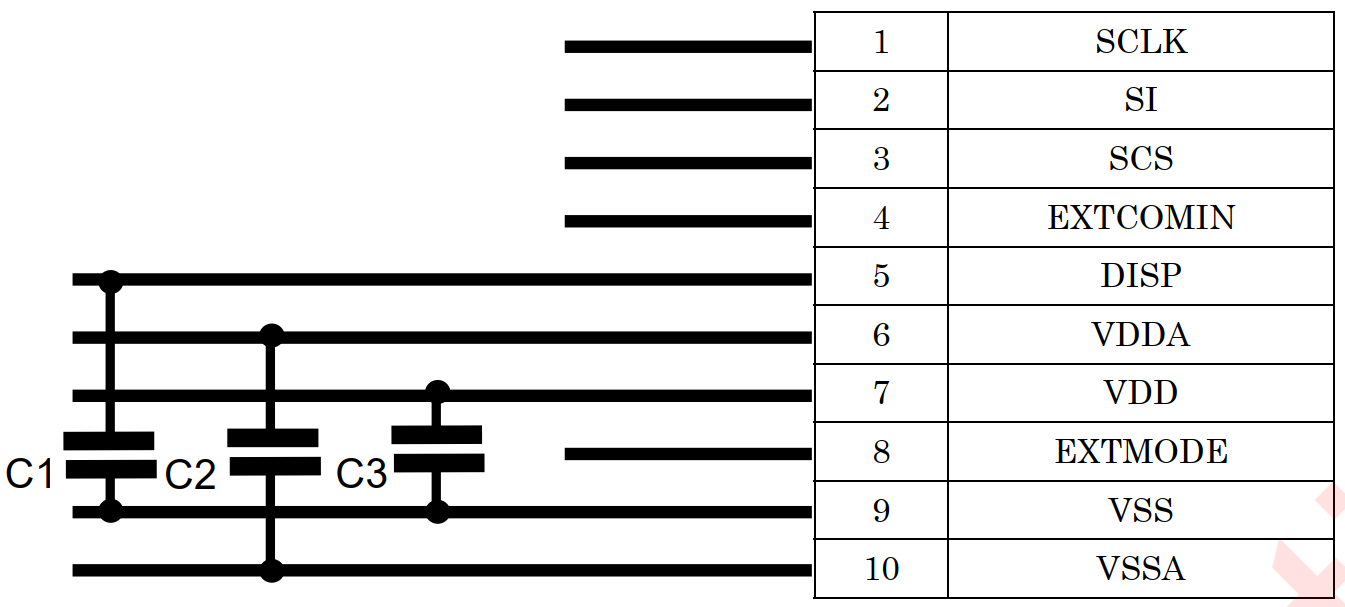
\includegraphics[width=0.8\textwidth]{Include/Figure/comp/LS011B7DH03_ext_capa.png}
	\caption{Typical Application Circuit - Source: \textit{LS011B7DH03}\cite{LS011B7DH03}}
	\label{fig:LS011B7DH03_ext_capa}
\end{figure}

The \textit{LS011B7DH03} have a very simple integration process and only requires three external capacitor ceramic capacitors; $C_1$ $C_2$ and $C_3$, to filter power supply lines of the panel. The recommended capacitors are listed in table \ref{tab:LS011B7DH03_cap_recom_tab}.

\begin{table}[H]
\centering
\setlength{\extrarowheight}{2pt}
\begin{tabular}{|l|c|c|c|}\hline
\textbf{ID} & \textbf{Specification} & \textbf{Value} & \textbf{Unit} \\\hline
$C_1$ & Rank B ceramic capacitor & $560^{\tiny(1)}$ & \si{\pico\farad}\\\hline
$C_2$ & Rank B ceramic capacitor & $1.0$ & \si{\micro\farad}\\\hline
$C_3$ & Rank B ceramic capacitor & $1.0$ & \si{\micro\farad}\\\hline
\multicolumn{4}{c}{\footnotesize $(1)$: Must be adjusted to respect \textit{DISP} rise time limit (\SI{50}{\nano\second})}
\end{tabular}
\caption{External Capacitor Recommendation - Source: \textit{LS011B7DH03}\cite{LS011B7DH03}}
\label{tab:LS011B7DH03_cap_recom_tab}
\end{table}

\subsubsection{\textit{nice!view} breakout board for \textit{LS011B7DH03}}

\textsc{Nice Technologies LLC} sells breakout board for the \textit{LS011B7DH03}:  \textit{nice!view}. This has the advantage of making the display easier to order but it also guaranty to have an easy to implement solution for a prototype board. Mechanical characteristics and pinout are illustrated in the figure \ref{fig:niceview_pinout}:

\begin{figure}[H]
\begin{subfigure}{.72\textwidth}
	\centering
	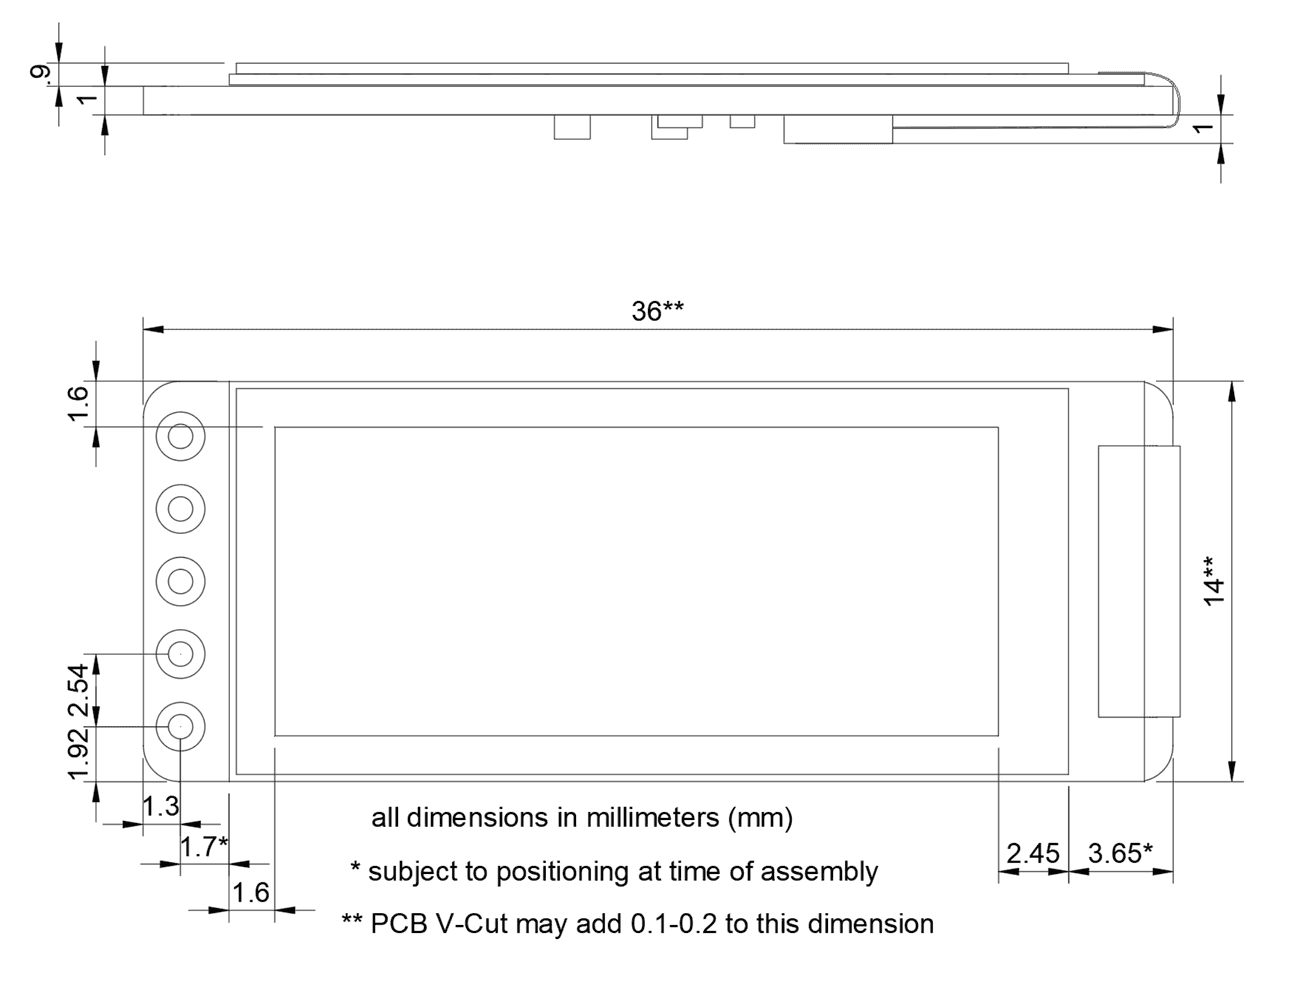
\includegraphics[width=1\textwidth]{Include/Figure/comp/niceview_dimensions.png}
	\caption{Dimensions}
	\end{subfigure}
\begin{subfigure}{.23\textwidth}
	\centering
	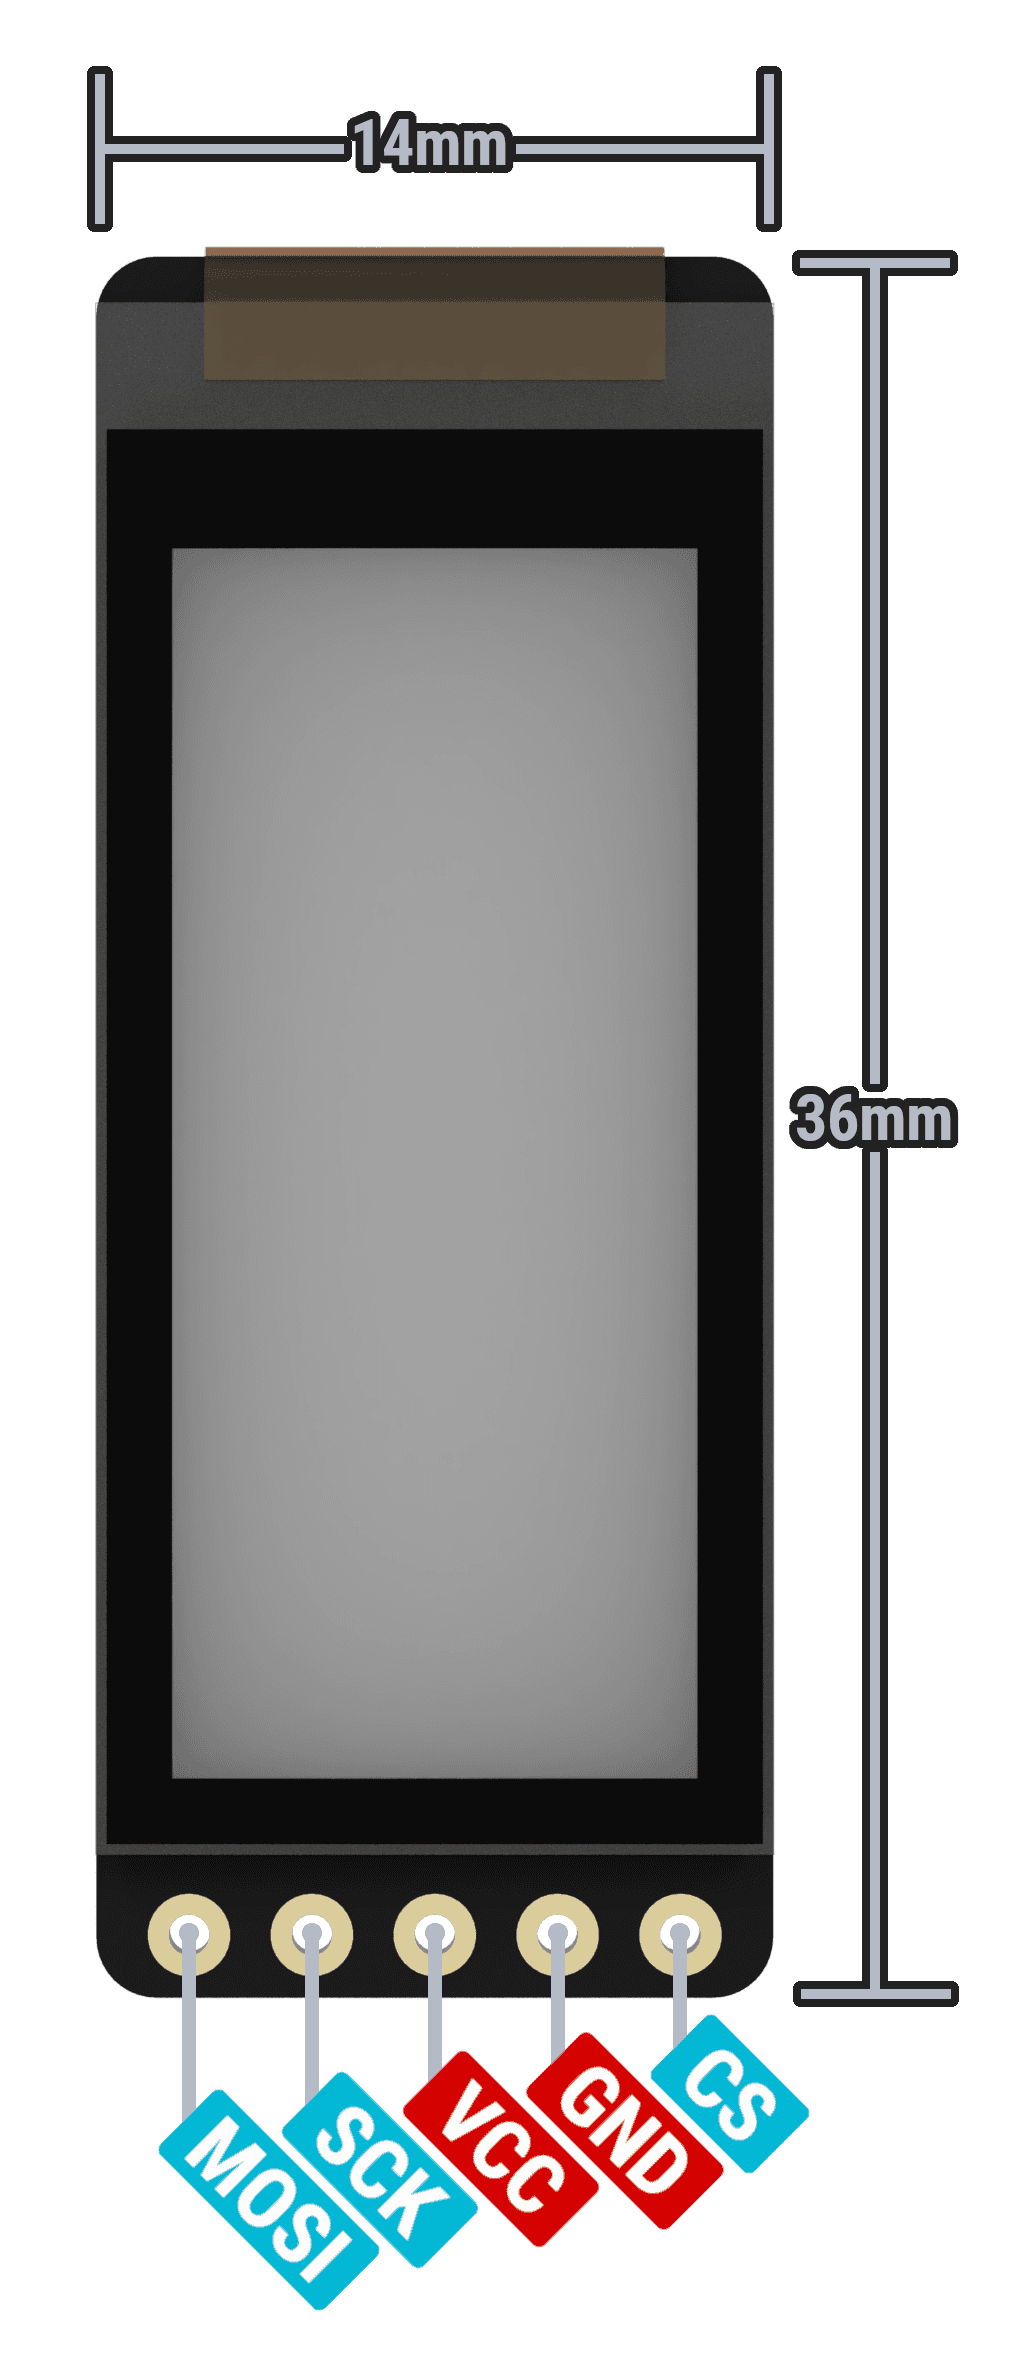
\includegraphics[width=1\textwidth]{Include/Figure/comp/niceview_pinout.png}
	\caption{Pinout}
	\end{subfigure}
	\caption{\textit{nice!view} Breakout Board for \textit{LS011B7DH03} - Source: \cite{niceview}}
	\label{fig:niceview_pinout}
\end{figure}

\textsc{Nice Technologies LLC} also provides an open source schematic of the textit{nice!view} breakout board for \textit{LS011B7DH03} illustrated in figures \ref{fig:niceview_schematic_1} to \ref{fig:niceview_schem} :

\begin{figure}[H]
	\centering
	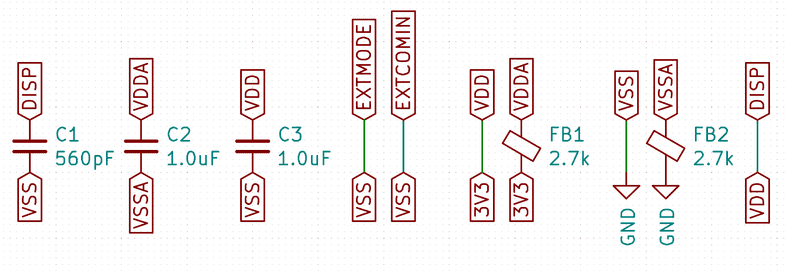
\includegraphics[width=0.65\textwidth]{Include/Figure/comp/niceview_schematic_1.png}
	\caption{\textit{nice!view} Electrical Schematic (Part 1) - Source: \cite{niceview}}
	\label{fig:niceview_schematic_1}
\end{figure}

\begin{figure}[H]
	\centering
\begin{subfigure}{.3\textwidth}
	\centering
	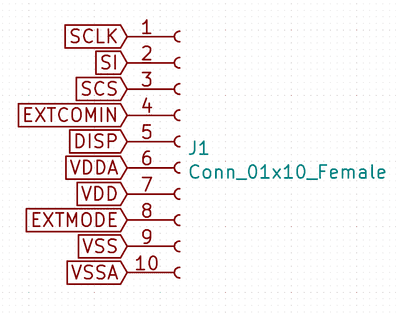
\includegraphics[width=1\textwidth]{Include/Figure/comp/niceview_schematic_2.png}
	\end{subfigure}
\begin{subfigure}{.3\textwidth}
	\centering
	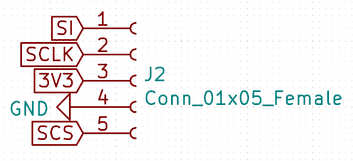
\includegraphics[width=1\textwidth]{Include/Figure/comp/niceview_schematic_3.png}
	\end{subfigure}
	\caption{\textit{nice!view} Electrical Schematic (Part 2) - Source: \cite{niceview}}
	\label{fig:niceview_schem}
\end{figure}

%-------------------------------------------------------------------------------------
\subsection{GNSS Receiver - MAX-M10S}

Figure \ref{fig:maxm10s_pict} illustrate the \textit{MAX-M10S} module from \textsc{u-blox}:

\begin{figure}[H]
	\centering
	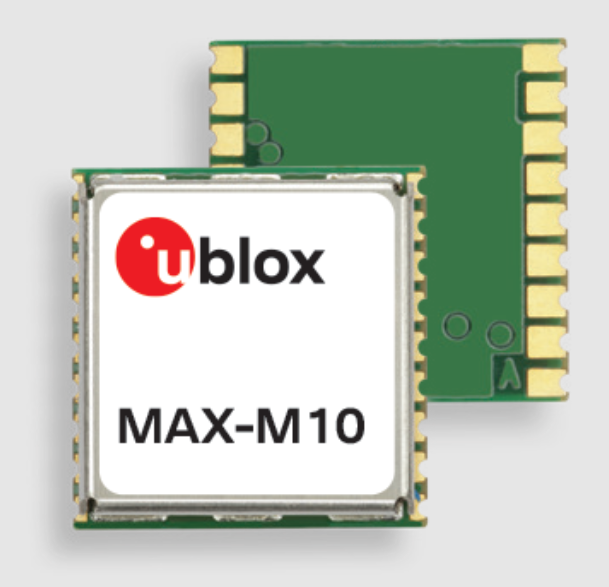
\includegraphics[width=0.25\textwidth]{Include/Figure/comp/maxm10s_pict.png}
	\caption{Module \textit{MAX-M10S} from \textsc{u-blox} - Source: \cite{MAXM10S}}
	\label{fig:maxm10s_pict}
\end{figure}
\;\\[-20pt]
As mentioned in the system decomposition, the choice was made to integrate an external \textit{GNSS} receiver to the device. After researches for suitable solutions, the most interesting solution seamed to be the last \textit{M10} series from \textit{u-blox}.

\;\\[-40pt]
\subsubsection{Introduction to \textsc{u-blox} \textit{M10} series:}

The \textit{M10}\cite{ublox_m10} series is the tenth generation of standard precision \textit{GNSS} technology platform form \textsc{u-blox}. The \textit{M10} series offers ultra-low-power positioning in an ultra-compact form factor with solid accuracy and good availability. This series is advertised to consume less than \SI{15}{\milli\watt} in continuous tracking mode and high RF sensitivity which guarantees a short time to establish a position. The \textit{M10} platform was specifically designed for small battery-powered wearable applications.\\

The \textit{M10} series form \textsc{u-blox} is ideal for compact product design and smart-watches by providing interesting features, such as: 
\begin{itemize}
\item \textbf{RF interference mitigation (\textit{RIM})}: Technique to protect \textit{GNSS} receivers from interference and jamming without compromising final position, velocity and timing accuracy \cite{rf_inter_mit}. \textit{RIM} gives protection against:
\begin{itemize}
\item \textbf{Advanced jamming}: Intentional and deliberate interference by radiation of electromagnetic signals at \textit{GNSS} frequencies \cite{jamming}.
\item \textbf{Spoofing}: Malicious and deliberate practice of altering a user's \textit{GNSS} measurements, making positioning unreliable \cite{spoofing}.
\end{itemize}
\item \textbf{Super-S technology:} Boost performance in weak signal environments or when used with small antennas.
\end{itemize}

\;\\[-60pt]
\subsubsection{Description:}

Following the datasheet\cite{MAXM10S} of the \textit{MAX-M10S} \textit{GNSS} receiver module from \textsc{u-blox}, here is an overview of the module:

\begin{itemize}
\item The \textit{MAX-M10S} is built on the ultra low power \textsc{u-blox} \textit{M10 GNSS} platform and provide extremely good performances for all \textit{L1} \textit{GNSS} systems.
\item Power consumption lower than \SI{25}{\milli\watt} in continuous tracking mode, which allows great for all battery-operated devices.
\item Supports concurrent reception of four \textit{GNSS} (\textit{GPS, GLONASS, Galileo, and BeiDou}) for maximum position availability by selection of best available signal. This gives better reliability in challenging conditions like urban environment.
\item \textsc{u-blox} \textit{Super-S} technology offers excellent sensitivity with small antennas and is claiming to be able to improve the dynamic position accuracy by up to \SI{25}{\percent} in a a non-line-of-sight scenario.
\item The module integrates an \textit{LNA} and a \textit{SAW} filter in the RF path to improve sensitivity for design with passive antenna.
\item Provides advanced spoofing and jamming detection
\item Offer backwards pin-to-pin compatibility with previous \textsc{u-blox} generations which is interesting for design upgrade.
\item Compact module: $\SI{10.1}{\milli\meter} \times \SI{9.7}{\milli\meter}$
\end{itemize}

\subsubsection{Performance:}

The general performance of the \textit{MAX-M10S} module is described in table \ref{tab:maxm10s_perf_tab}:

\begin{table}[H]
	\centering
	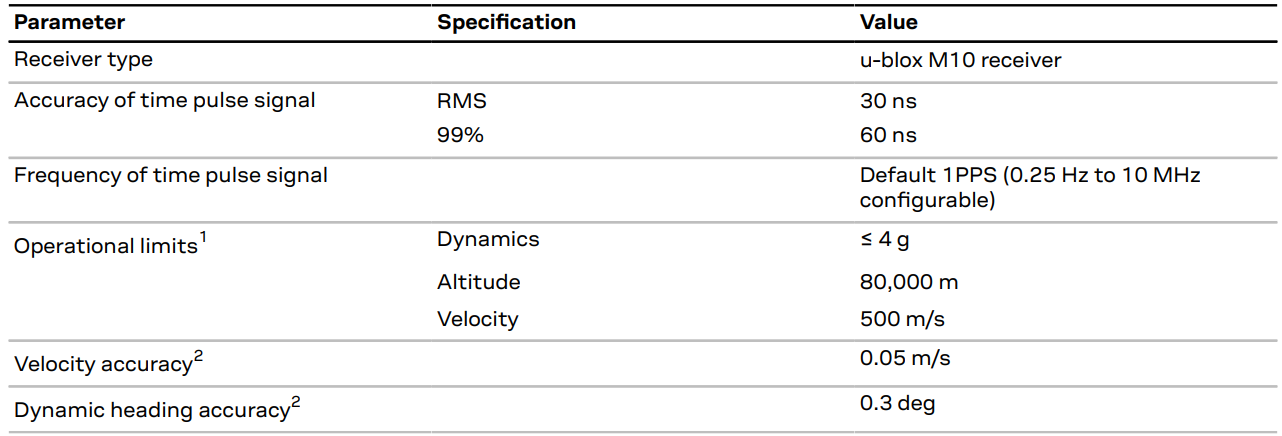
\includegraphics[width=1\textwidth]{Include/Figure/comp/maxm10s_perf_tab.png}
\caption{\textit{MAX-M10S} - General Performance - Source: \cite{MAXM10S}}
\label{tab:maxm10s_perf_tab}
\end{table}

\pagebreak

The typical performance in multi-constellation \textit{GNSS} modes of the \textit{MAX-M10S} module is presented in table \ref{tab:maxm10s_typ_perf_mulit_const}:

\begin{table}[H]
\centering
\begin{subfigure}{\textwidth}
	\centering
	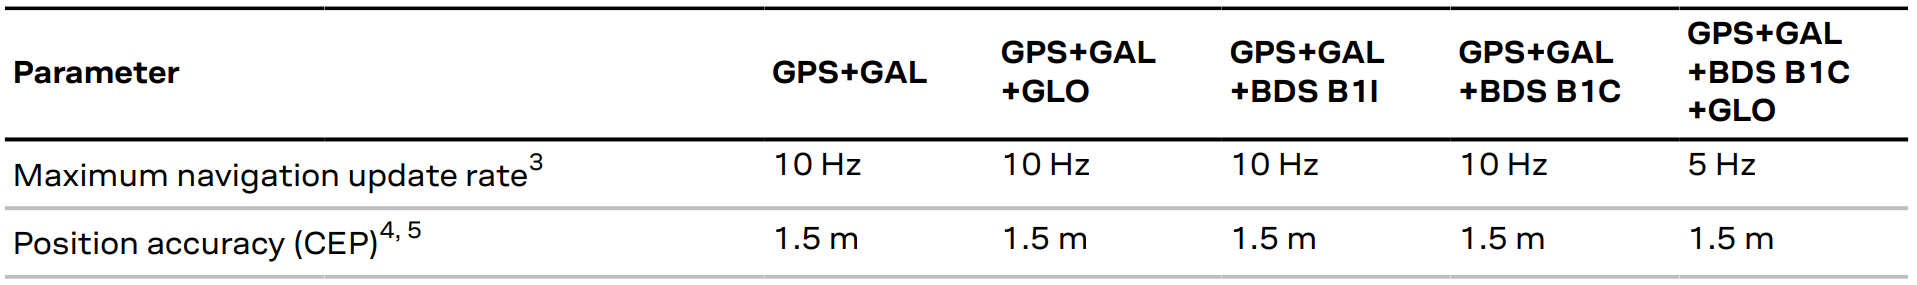
\includegraphics[width=1\textwidth]{Include/Figure/comp/maxm10s_typ_perf_mulit_const2.png}
\end{subfigure}
\begin{subfigure}{\textwidth}
	\centering
	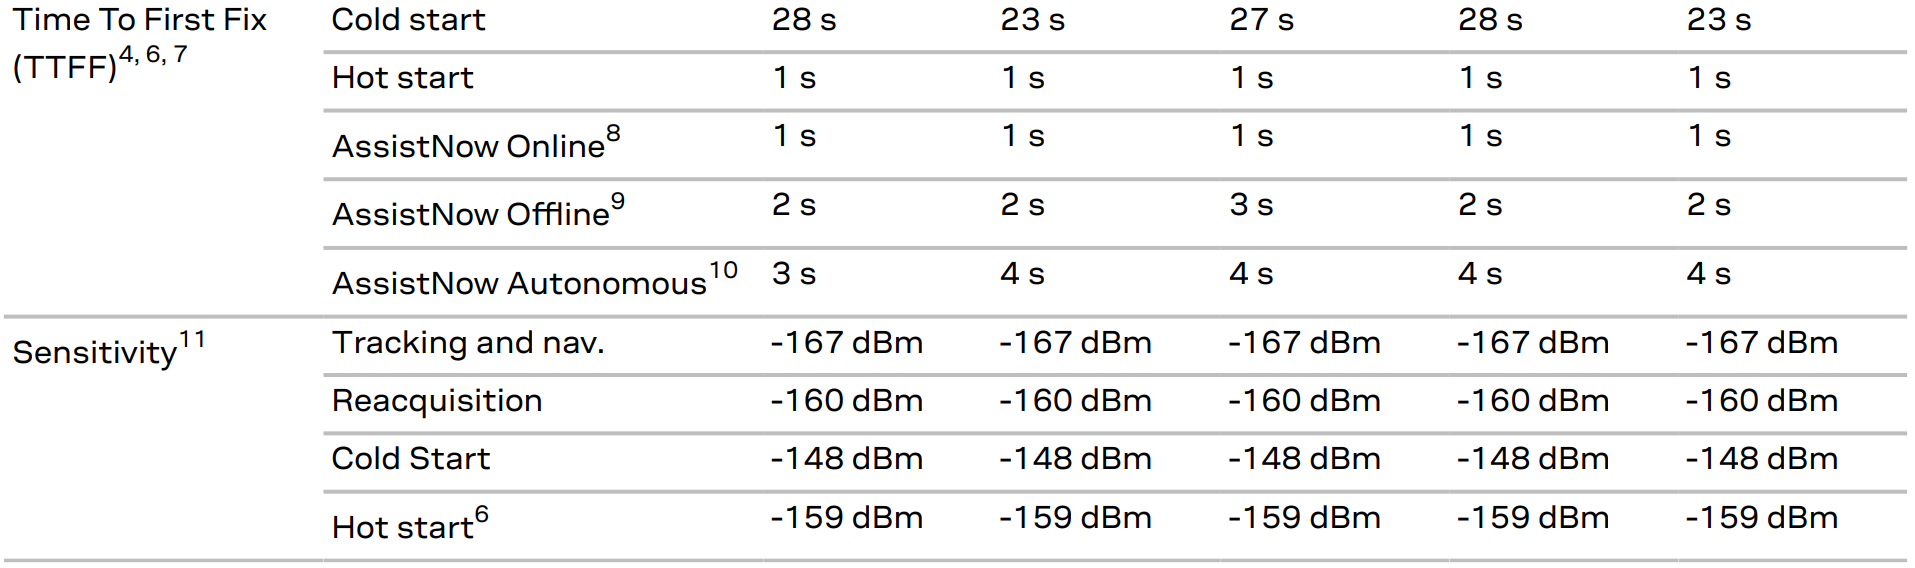
\includegraphics[width=1\textwidth]{Include/Figure/comp/maxm10s_typ_perf_mulit_const1.png}
\end{subfigure}
\begin{subfigure}{\textwidth}
	\centering
	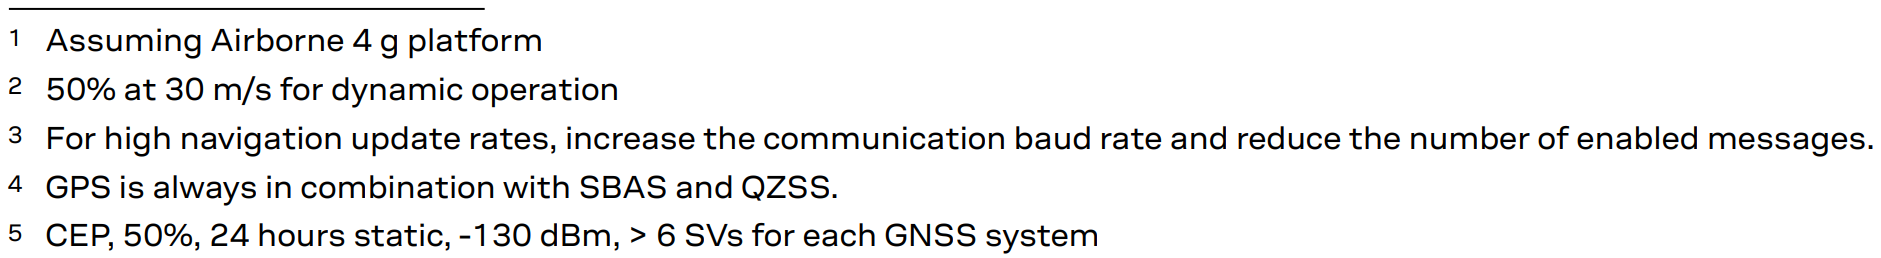
\includegraphics[width=1\textwidth]{Include/Figure/comp/maxm10s_typ_perf_mulit_const3.png}
\end{subfigure}
\caption{Typical Performance in Multi-constellation Modes - Source: \cite{MAXM10S}}
\label{tab:maxm10s_typ_perf_mulit_const}
\end{table}

The typical typical performance in single-\textit{GNSS} mode of the \textit{MAX-M10S} module is presented in table \ref{tab:maxm10s_typ_perf_mulit_const}:

\begin{table}[H]
	\centering
	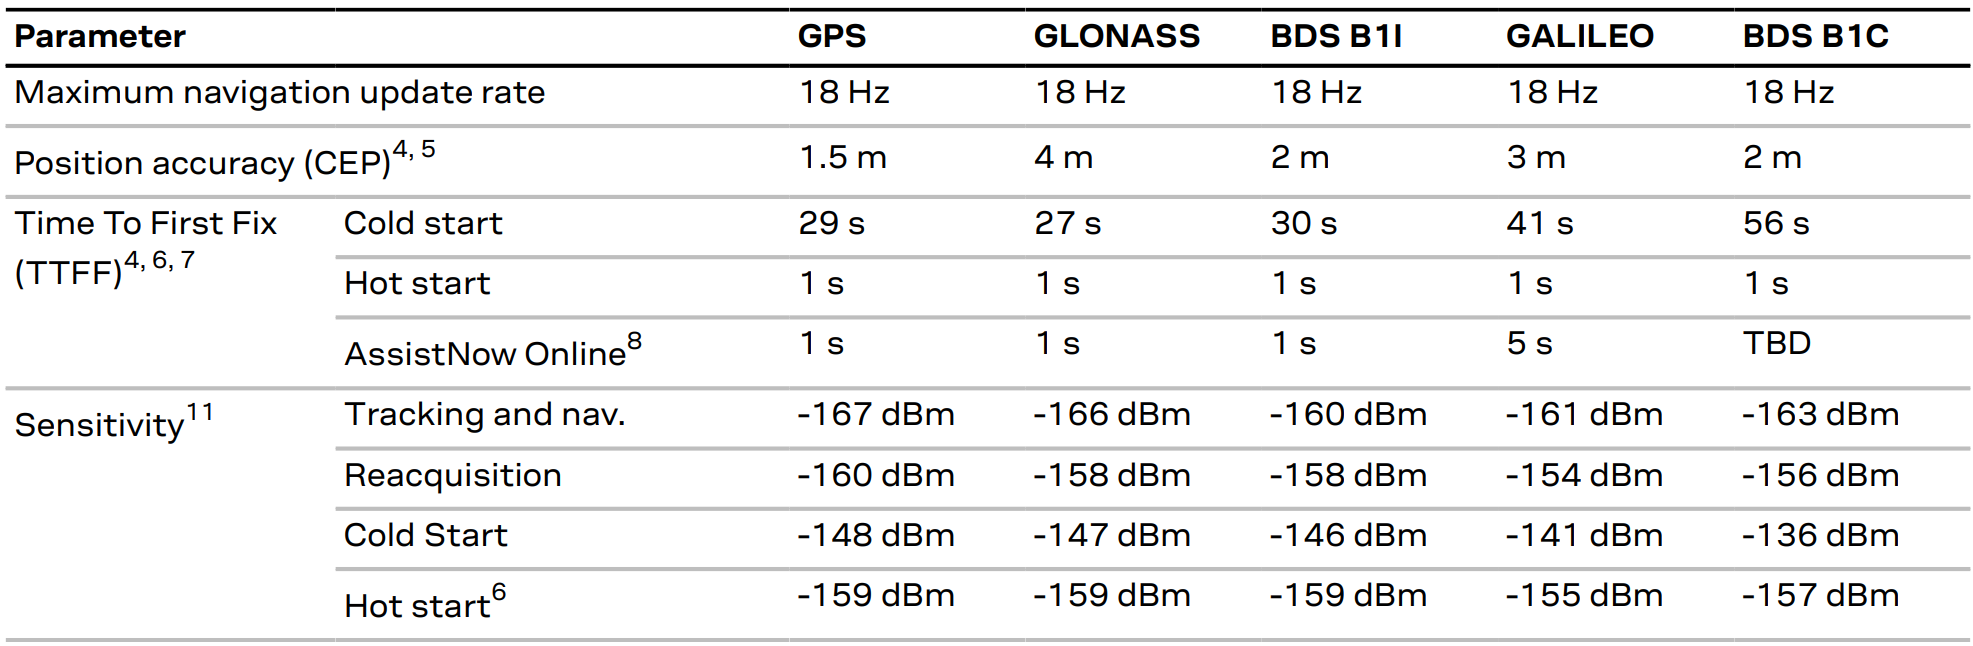
\includegraphics[width=1\textwidth]{Include/Figure/comp/maxm10s_typ_perf_single_gnss.png}
\caption{Typical Performance in Single-\textit{GNSS} Mode - Source: \cite{MAXM10S}}
\label{tab:maxm10s_typ_perf_single_gnss}
\end{table}

\subsubsection{Supported \textit{GNSS} Constellations:}

As mentioned earlier, the \textit{MAX-M10S} is a concurrent \textit{GNSS} receiver and can receive and track multiple \textit{GNSS} systems. The concurrent reception of multiple \textit{GNSS} constellations are enabled by the single RF front-end architecture. It is possible to achieve lower power consumption by configuring the \textit{GNSS} receiver for a subset of constellations.
\textbf{By default}, the configuration of the \textit{\textit{MAX-M10S}} is concurrent reception of \textbf{\textit{GPS}}, \textbf{\textit{Galileo}}, and \textbf{\textit{BeiDou B1I}} with \textbf{\textit{QZSS}} and \textbf{\textit{SBAS}} enabled.\\

Supported \textit{GNSS} and signals on \textit{MAX-M10S} are listed in table \ref{tab:maxm10s_support_sign}:

\begin{table}[H]
\centering
\begin{subfigure}{\textwidth}
	\centering
	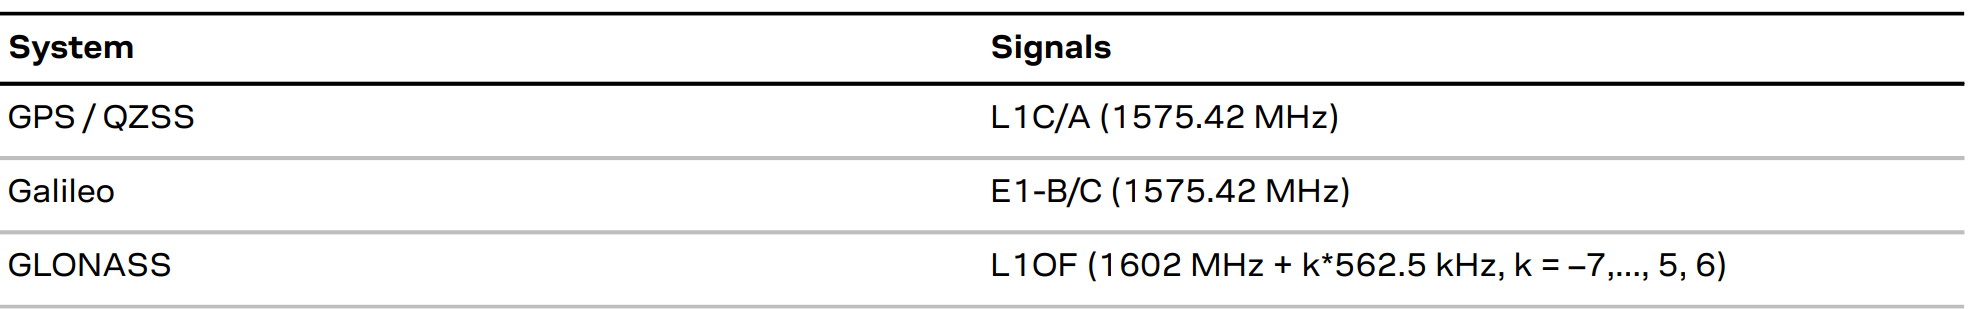
\includegraphics[width=1\textwidth]{Include/Figure/comp/maxm10s_support_sign.png}
\end{subfigure}
\begin{subfigure}{\textwidth}
	\centering
	
\includegraphics[width=1\textwidth]{Include/Figure/comp/maxm10s_support_sign2.png}
\end{subfigure}
\begin{subfigure}{\textwidth}
	\centering
	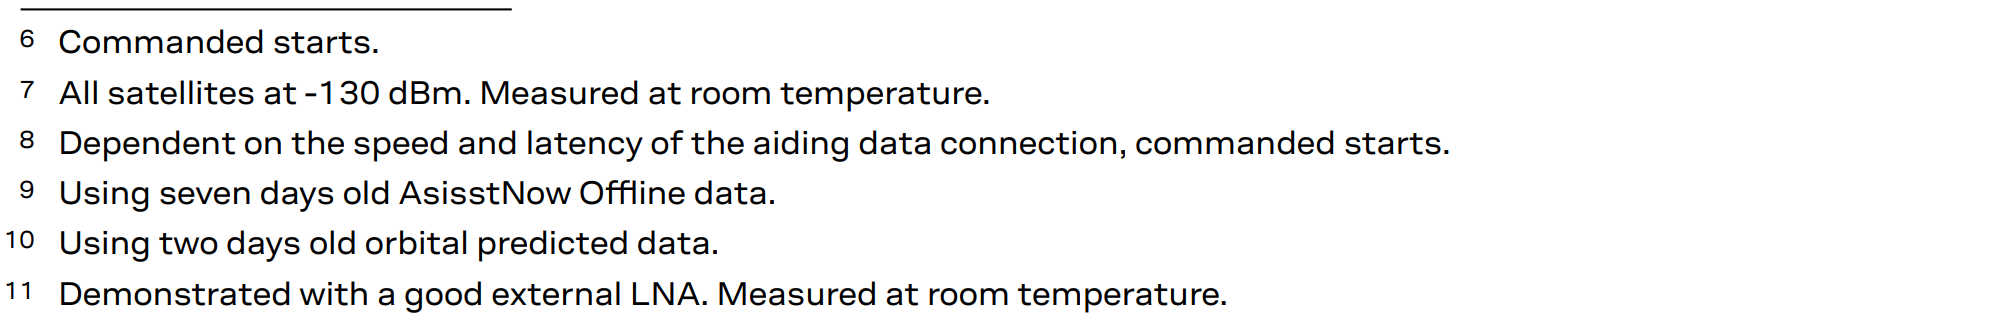
\includegraphics[width=1\textwidth]{Include/Figure/comp/maxm10s_support_sign3.png}
\end{subfigure}
\caption{Supported \textit{GNSS} and Signals on \textit{MAX-M10S} - Source: \cite{MAXM10S}}
\label{tab:maxm10s_support_sign}
\end{table}

Supported Assisted (\textit{A-GNSS}) service on \textit{MAX-M10S} are listed in table \ref{tab:maxm10s_support_assist_serv}:

\begin{table}[H]
	\centering
	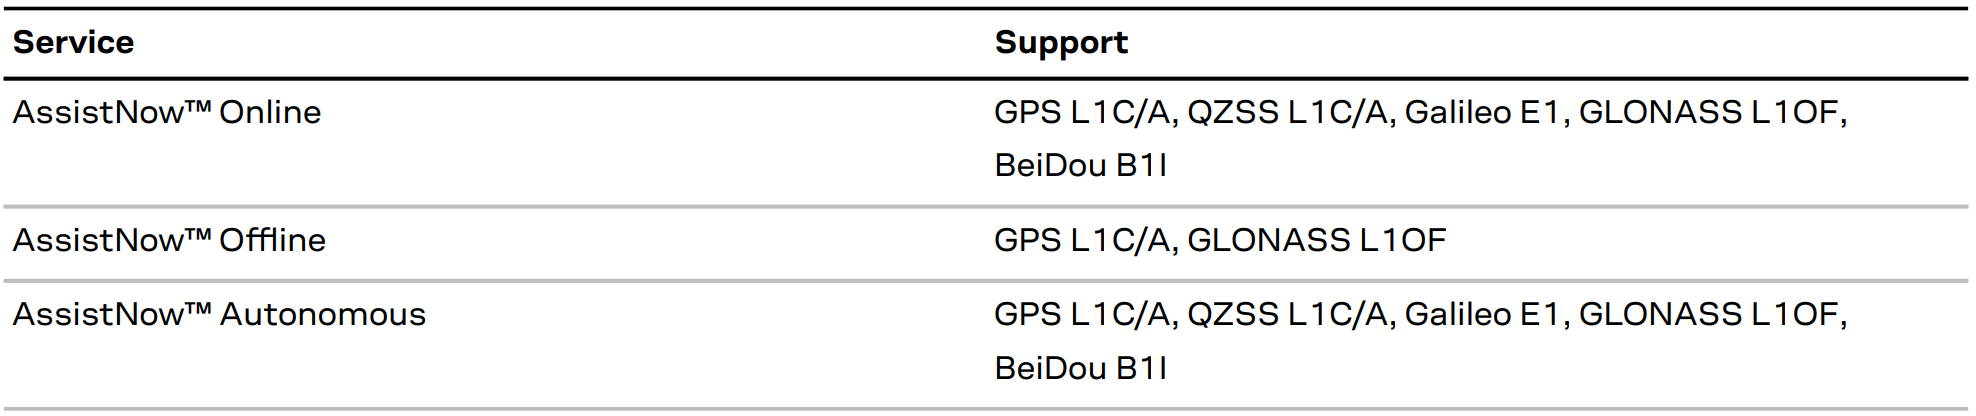
\includegraphics[width=1\textwidth]{Include/Figure/comp/maxm10s_support_assist_serv.png}
\caption{\textit{MAX-M10S} - Supported Assisted \textit{A-GNSS} service - Source: \cite{MAXM10S}}
\label{tab:maxm10s_support_assist_serv}
\end{table}

Supported augmentation systems on \textit{MAX-M10S} are listed in table \ref{tab:maxm10s_support_augnm_sys}:

\begin{table}[H]
	\centering
	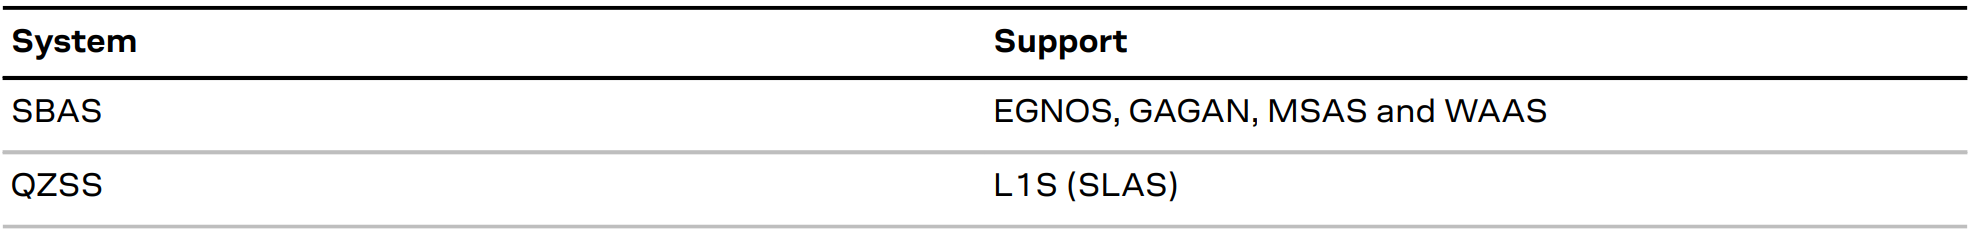
\includegraphics[width=1\textwidth]{Include/Figure/comp/maxm10s_support_augnm_sys.png}
\caption{\textit{MAX-M10S} - Supported Augmentation Systems - Source: \cite{MAXM10S}}
\label{tab:maxm10s_support_augnm_sys}
\end{table}

\warning{\begin{itemize}[$\rightarrow$]
\item [\textbf{Note:}]
\item The augmentation systems \textit{SBAS} and \textit{QZSS} can be enabled only if \textit{GPS} operation is also enabled.
\end{itemize}}
\pagebreak
\subsubsection{Supported Protocols:}

Supported protocols on \textit{MAX-M10S} are listed in table \ref{tab:maxm10s_support_proto}:

\begin{table}[H]
	\centering
	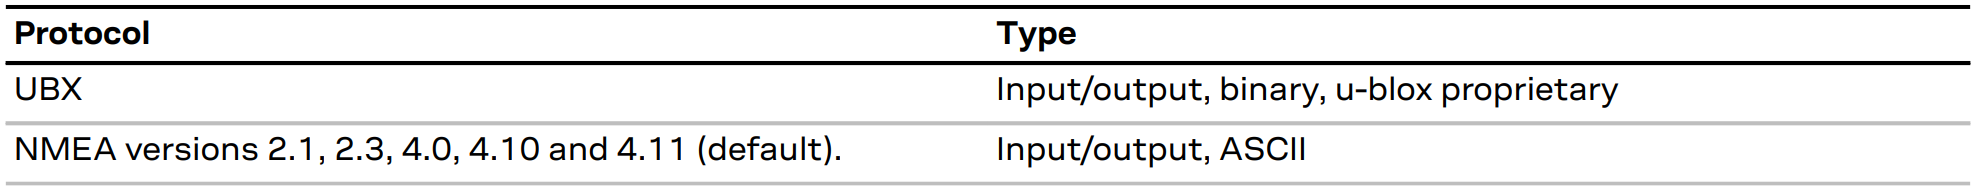
\includegraphics[width=1\textwidth]{Include/Figure/comp/maxm10s_support_proto.png}
\caption{\textit{MAX-M10S} - Supported Protocols - Source: \cite{MAXM10S}}
\label{tab:maxm10s_support_proto}
\end{table}

\subsubsection{Firmware Features:}
The detailed description of firmware features offered on the \textit{MAX-M10S} are listed in table \ref{tab:maxm10s_firm_feature}:

\begin{table}[H]
	\centering
\begin{subfigure}{\textwidth}
	\centering
	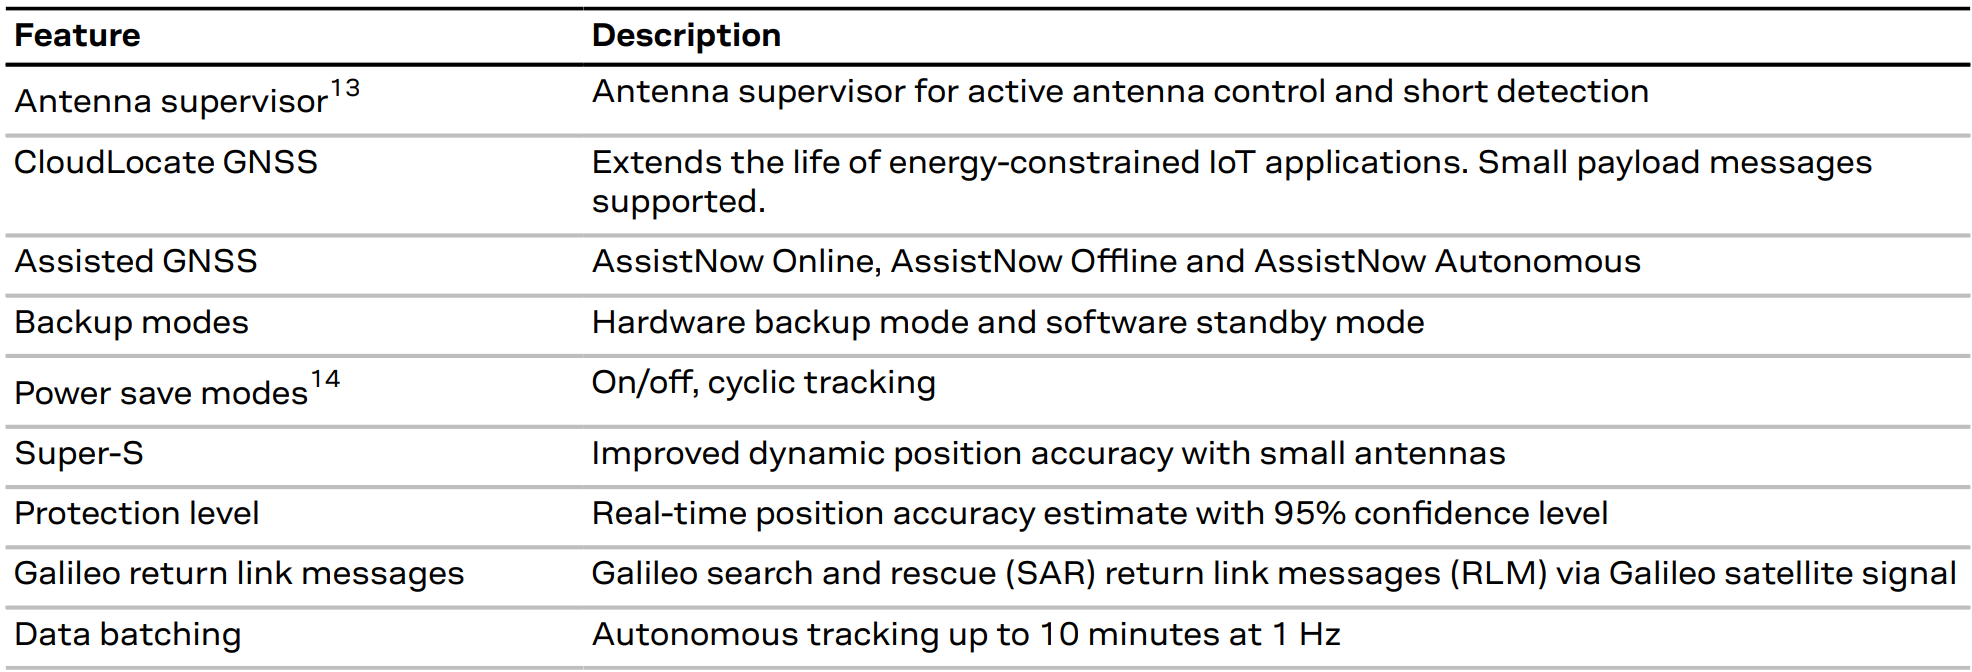
\includegraphics[width=1\textwidth]{Include/Figure/comp/maxm10s_firm_feature.png}
\end{subfigure}
\begin{subfigure}{\textwidth}
	\centering
	
\includegraphics[width=1\textwidth]{Include/Figure/comp/maxm10s_firm_feature2.png}
\end{subfigure}
\begin{subfigure}{\textwidth}
	\centering
	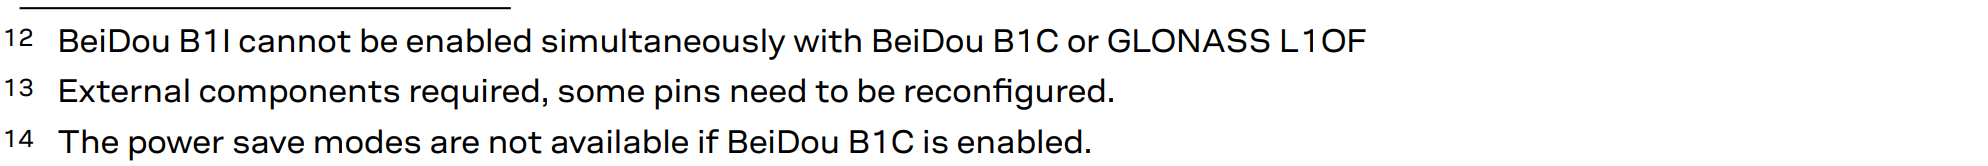
\includegraphics[width=1\textwidth]{Include/Figure/comp/maxm10s_firm_feature3.png}
\end{subfigure}
\caption{\textit{MAX-M10S} - Firmware Features - Source: \cite{MAXM10S}}
\label{tab:maxm10s_firm_feature}
\end{table}

The security features offered by the \textit{MAX-M10S} are listed in table \ref{tab:maxm10s_firm_feature}:

\begin{table}[H]
	\centering
	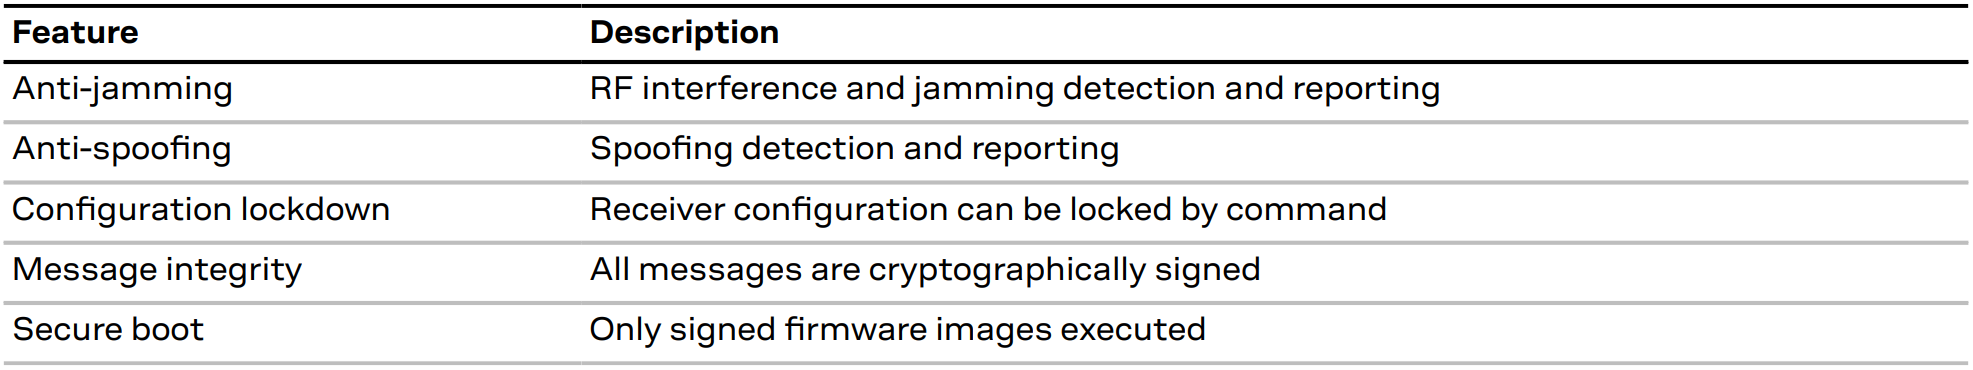
\includegraphics[width=1\textwidth]{Include/Figure/comp/maxm10s_sec_feat.png}
\caption{\textit{MAX-M10S} - Security Features - Source: \cite{MAXM10S}}
\label{tab:maxm10s_sec_feat}
\end{table}

\pagebreak
\;\\[-60pt]
\subsubsection{Block Diagram:}

Figure \ref{fig:maxm10s_bloc_diag} illustrate the block diagram of the \textit{MAX-M10S} \textit{GNSS} receiver:

\begin{figure}[H]
	\centering
	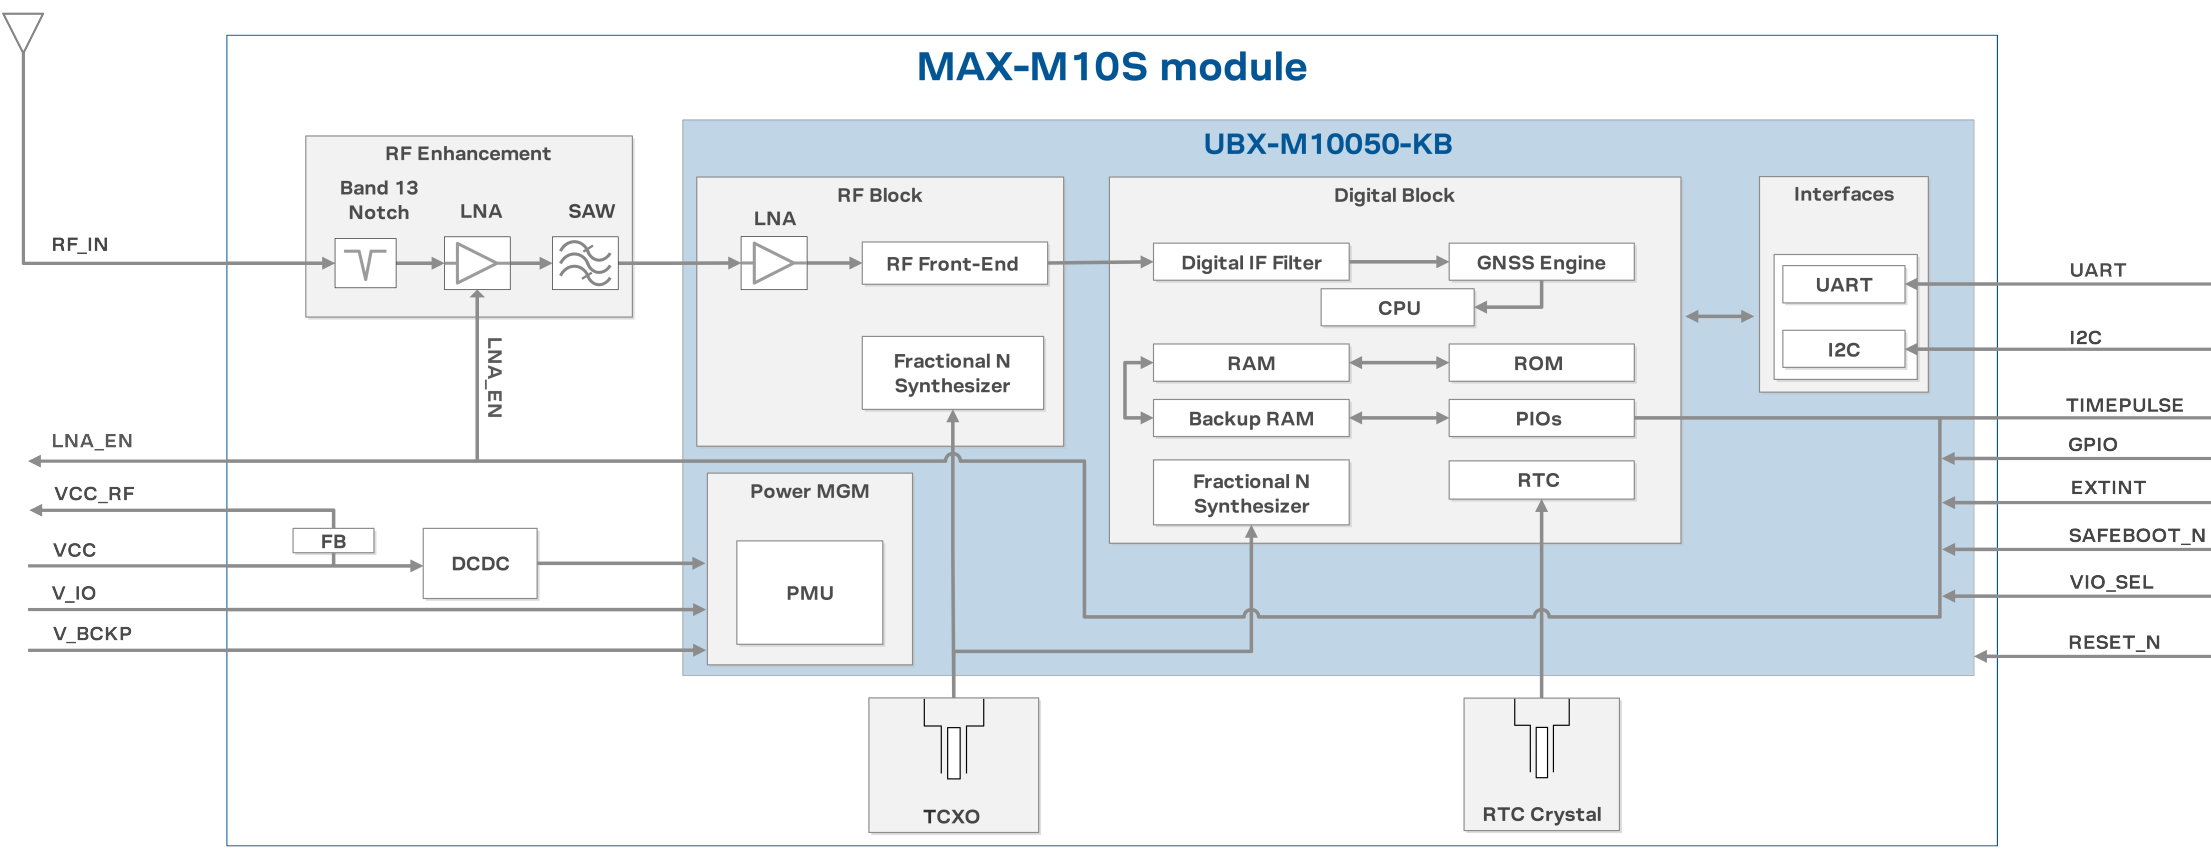
\includegraphics[width=1\textwidth]{Include/Figure/comp/maxm10s_bloc_diag.png}
	\caption{\textit{MAX-M10S} - Block Diagram - Source: \cite{MAXM10S}}
	\label{fig:maxm10s_bloc_diag}
\end{figure}

The most notable blocks of the \textit{MAX-M10S} shown in figure \ref{fig:maxm10s_bloc_diag} are:

\begin{itemize}
\item \textbf{RF Enhancement Block:} \\ The internal line of the module integrates a \textit{Band 13 Notch} filter, an \textit{LNA} and a \textit{SAW} filter.
\item \textbf{Power Management Block:} \\ A power management unit is integrated in the module.
\item \textbf{TCXO Block:} The module possesses a temperature controlled crystal oscillator that are more precise compared to regular crystal oscillator. This features improve the tracking accuracy.
\item \textbf{RTC Crystal Block:} \\ The module also integrates a \textit{RTC} which allows to keep a correct timing value even if the \textit{GNSS} reception is lost. This is true as long as the module is powered by a back-up battery.
\item \textbf{Interface Block:} \\ The module integrates both \textit{UART} and \textit{I2C} serial bus interface
\end{itemize}
\;\\[-45pt]
\subsubsection{Pin Definition:}

The pinout of the \textit{MAX-M10S} is illustrated in the figure \ref{fig:maxm10s_bloc_pinout}

\begin{figure}[H]
	\centering
	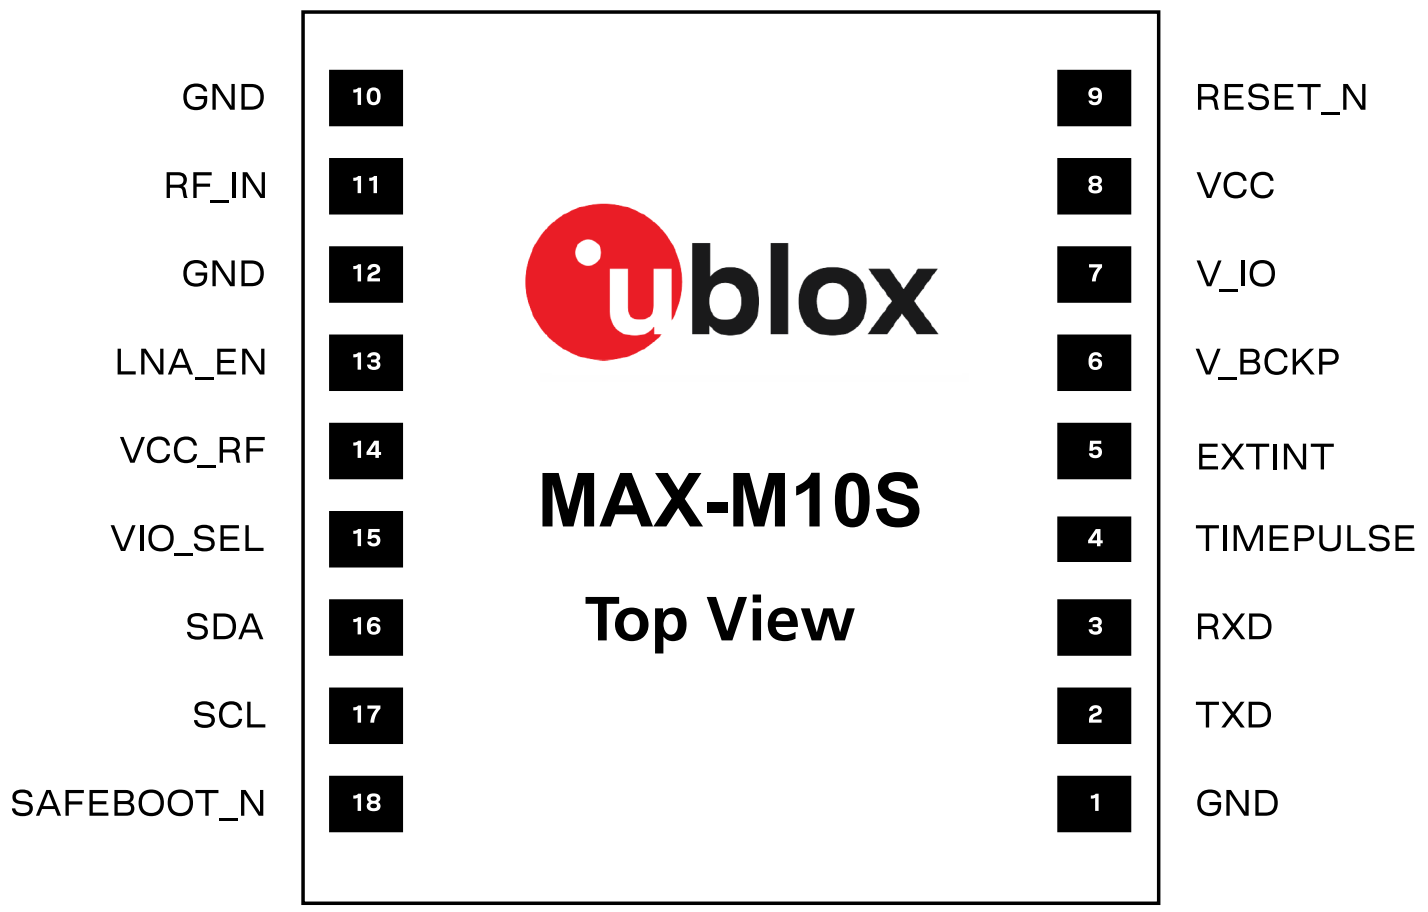
\includegraphics[width=0.45\textwidth]{Include/Figure/comp/maxm10s_bloc_pinout.png}
	\caption{\textit{MAX-M10S} - Pin Assignment - Source: \cite{MAXM10S}}
	\label{fig:maxm10s_bloc_pinout}
\end{figure}

The pin assignment and their function is described in table \ref{tab:maxm10s_bloc_pinout_tab}:

\begin{table}[H]
	\centering
	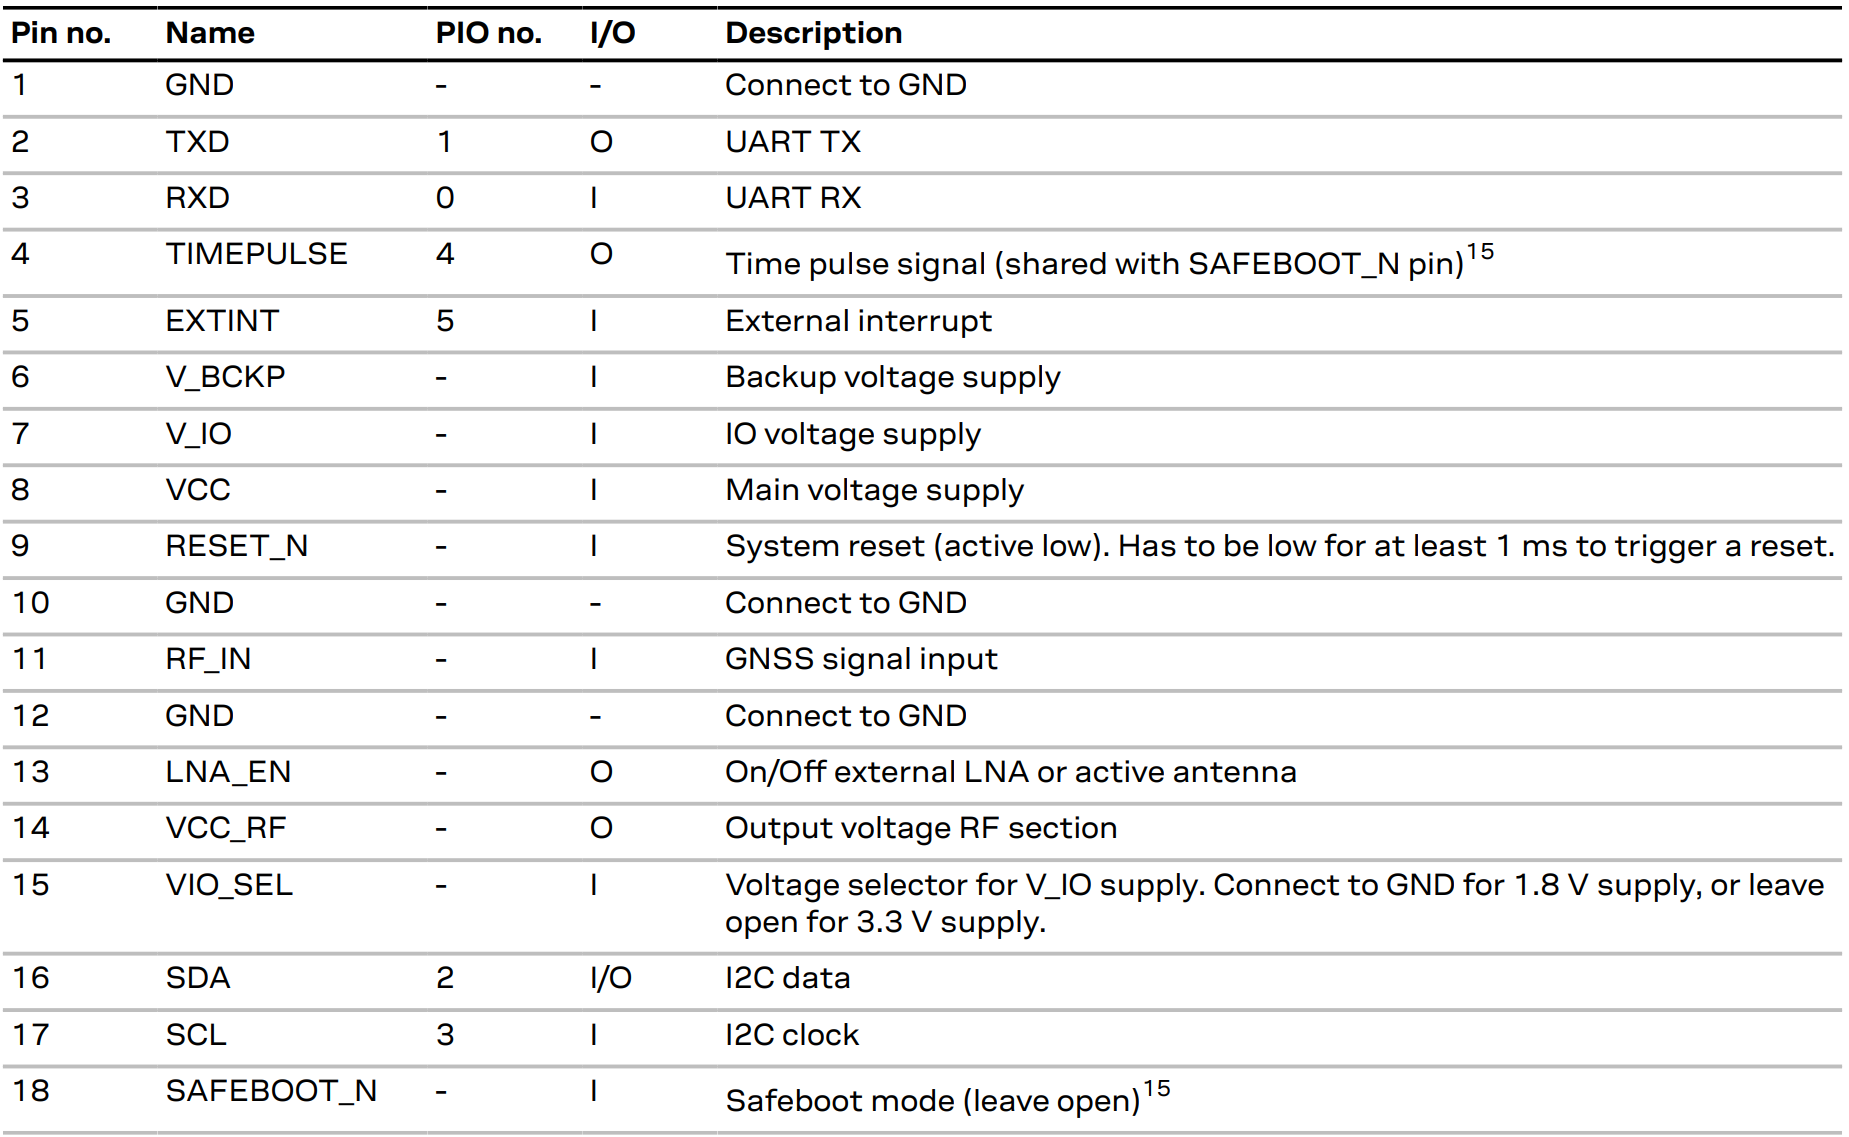
\includegraphics[width=1\textwidth]{Include/Figure/comp/maxm10s_bloc_pinout_tab.png}
\caption{\textit{MAX-M10S} - Pin Assignment Table - Source: \cite{MAXM10S}}
\label{tab:maxm10s_bloc_pinout_tab}
\end{table}

The description of pins state of the \textit{MAX-M10S} is presented in table \ref{tab:maxm10s_bloc_pinout_state_tab}:

\begin{table}[H]
	\centering
	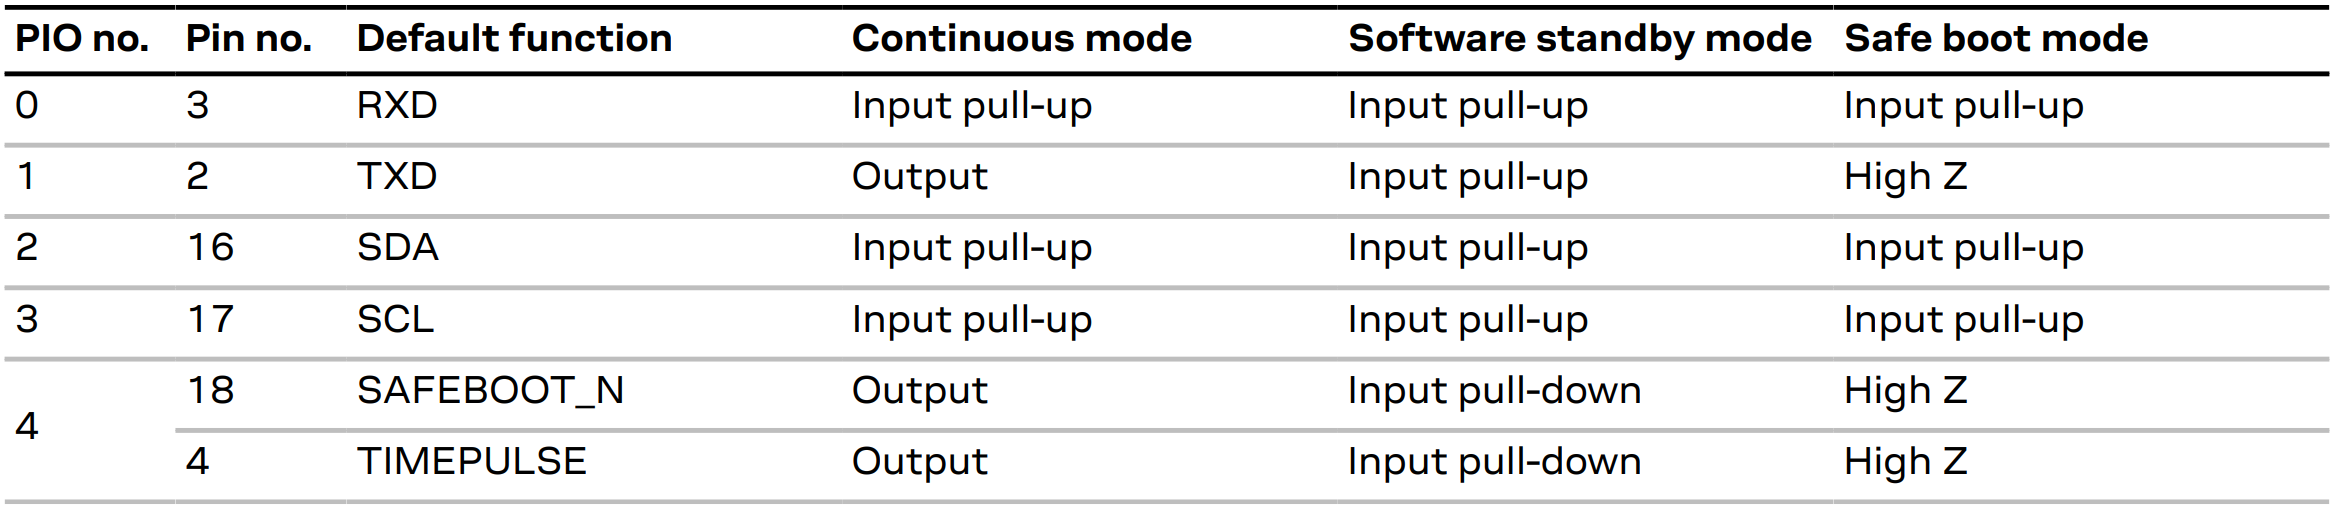
\includegraphics[width=1\textwidth]{Include/Figure/comp/maxm10s_bloc_pinout_state_tab.png}
\caption{\textit{MAX-M10S} - Pins State - Source: \cite{MAXM10S}}
\label{tab:maxm10s_bloc_pinout_state_tab}
\end{table}

\warning{
\begin{itemize}[$\quad \rightarrow$]
\item [\textbf{Note:}]
\item In reset mode (RESET\_N = \textit{low}), all PIOs are config. as input pull-up.
\item In hardware backup mode (VCC = \SI{0}{\volt} and V\_IO = \SI{0}{\volt} ), PIOs must not be driven.
\end{itemize}}
\pagebreak
\;\\[-60pt]
\subsubsection{Absolute Maximum Ratings:}
Absolute maximum ratings for the \textit{MAX-M10S} are listed in table \ref{tab:maxm10s_abs_max_tab}:

\begin{table}[H]
	\centering
	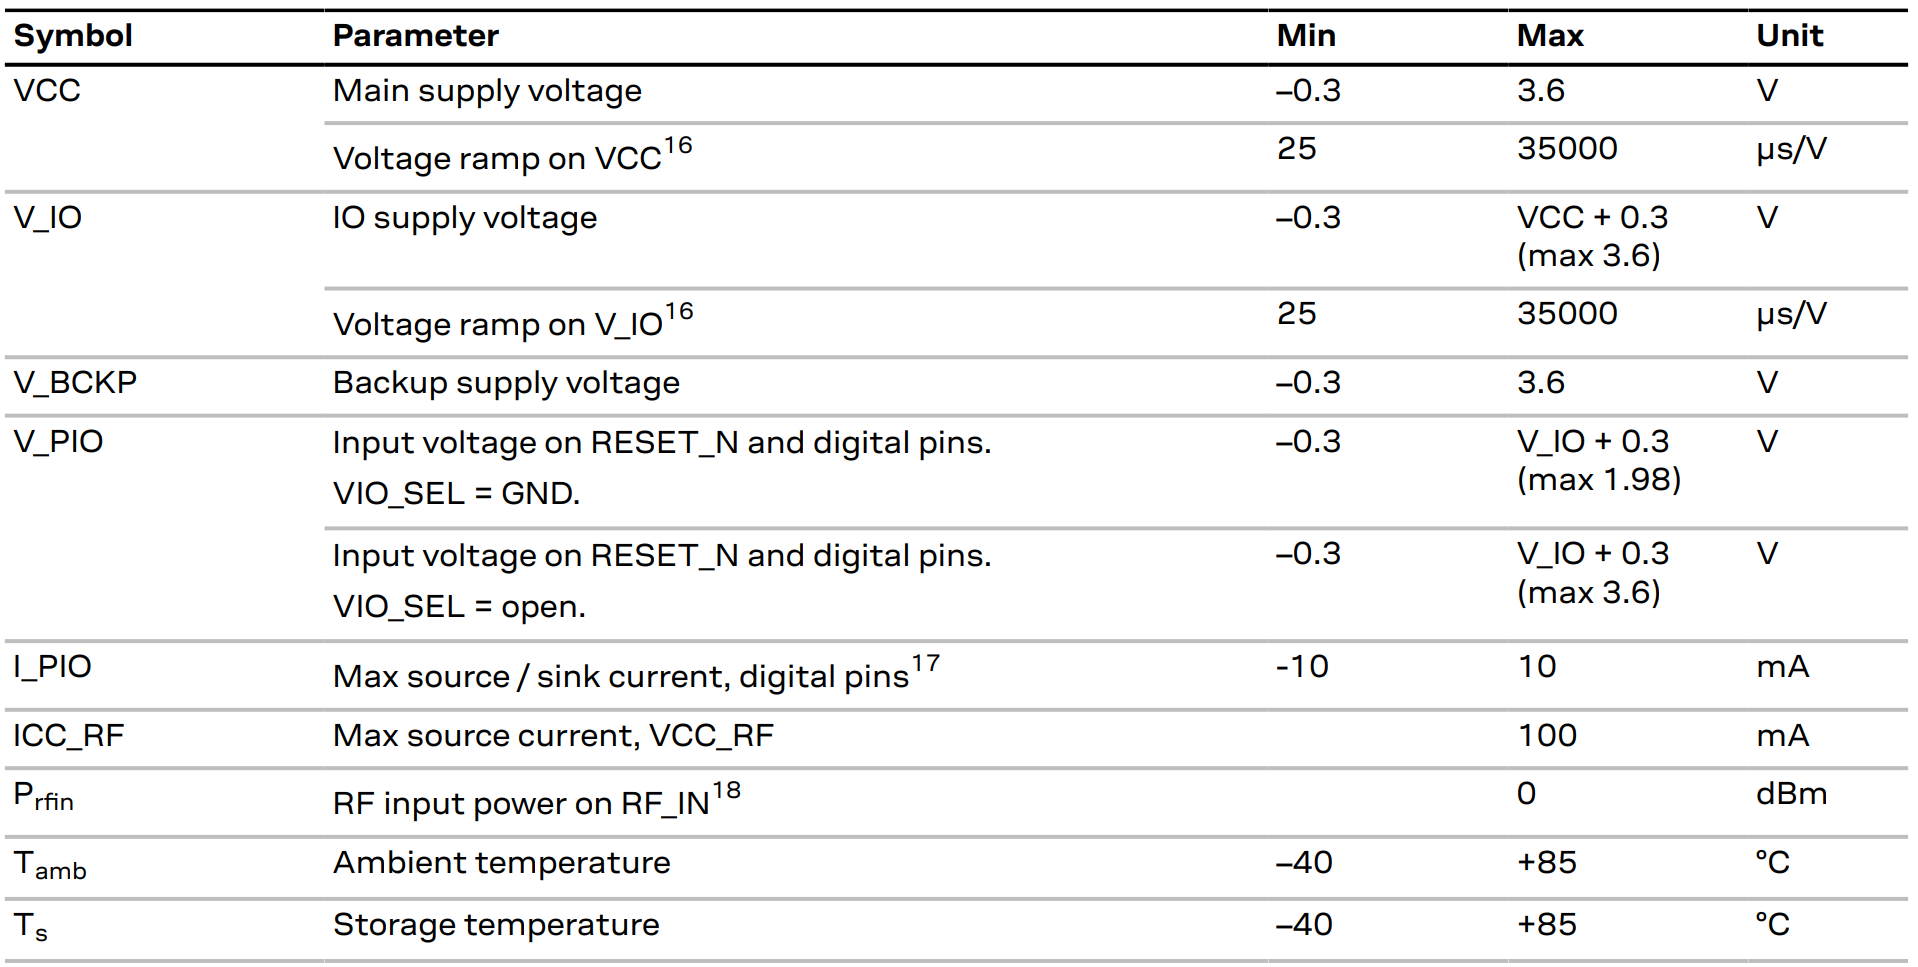
\includegraphics[width=1\textwidth]{Include/Figure/comp/maxm10s_abs_max_tab.png}
\caption{\textit{MAX-M10S} - Absolute Maximum Ratings - Source: \cite{MAXM10S}}
\label{tab:maxm10s_abs_max_tab}
\end{table}
\;\\[-45pt]
\warning{\begin{itemize}[\quad$\rightarrow$]
\item [\textbf{Note:}]
\item $V_{IO}$ supply voltage must not be higher than $V_{CC} + \SI{0.3}{\volt}$.
\item The product is not protected against over-voltage or reversed voltages. Voltage spikes exceeding the power supply voltage specification, given in table above, must be limited to values within the specified boundaries by using appropriate protection diodes.
\end{itemize}}
\;\\[-40pt]
\subsubsection{Recommended Operating Conditions:}

Recommended operating conditions for the \textit{MAX-M10S} are listed in table \ref{tab:maxm10s_recom_oper_tab}:

\begin{table}[H]
	\centering
	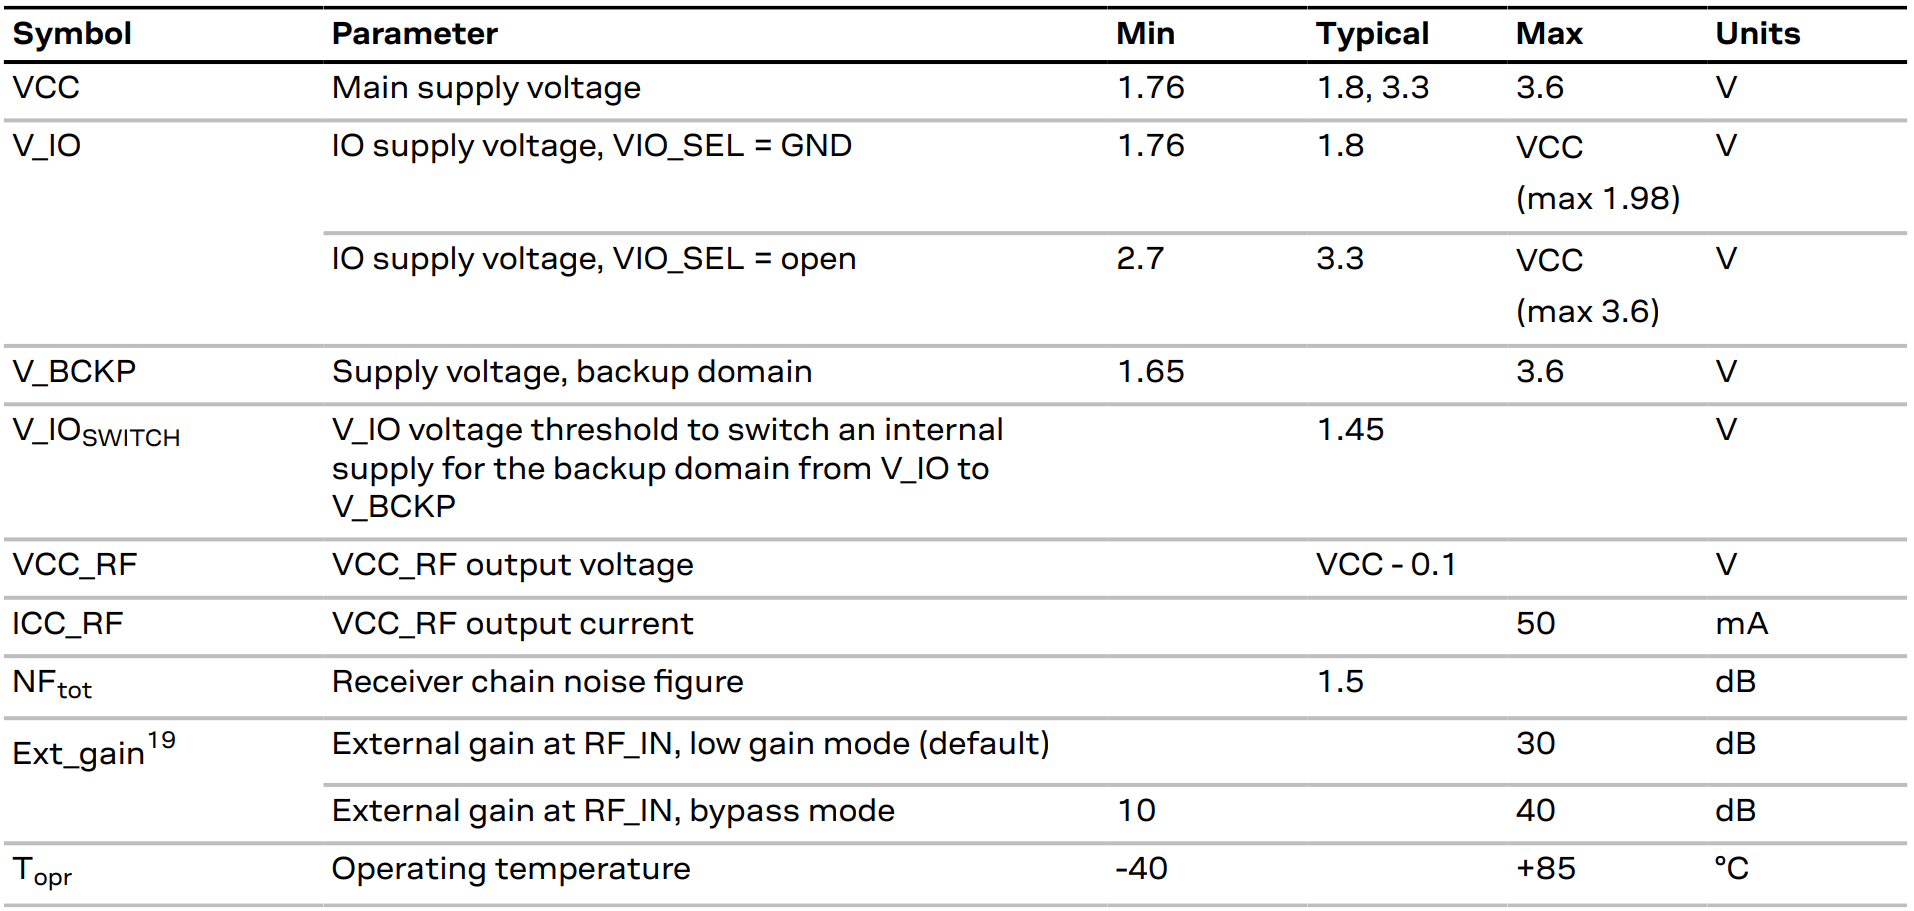
\includegraphics[width=1\textwidth]{Include/Figure/comp/maxm10s_recom_oper_tab.png}
\caption{\textit{MAX-M10S} - General Operating Conditions - Source: \cite{MAXM10S}}
\label{tab:maxm10s_recom_oper_tab}
\end{table}

Recommended digital IO conditions for the \textit{MAX-M10S} are listed in table \ref{tab:maxm10s_digit_io}:

\begin{table}[H]
\begin{subfigure}{\textwidth}
	\centering
	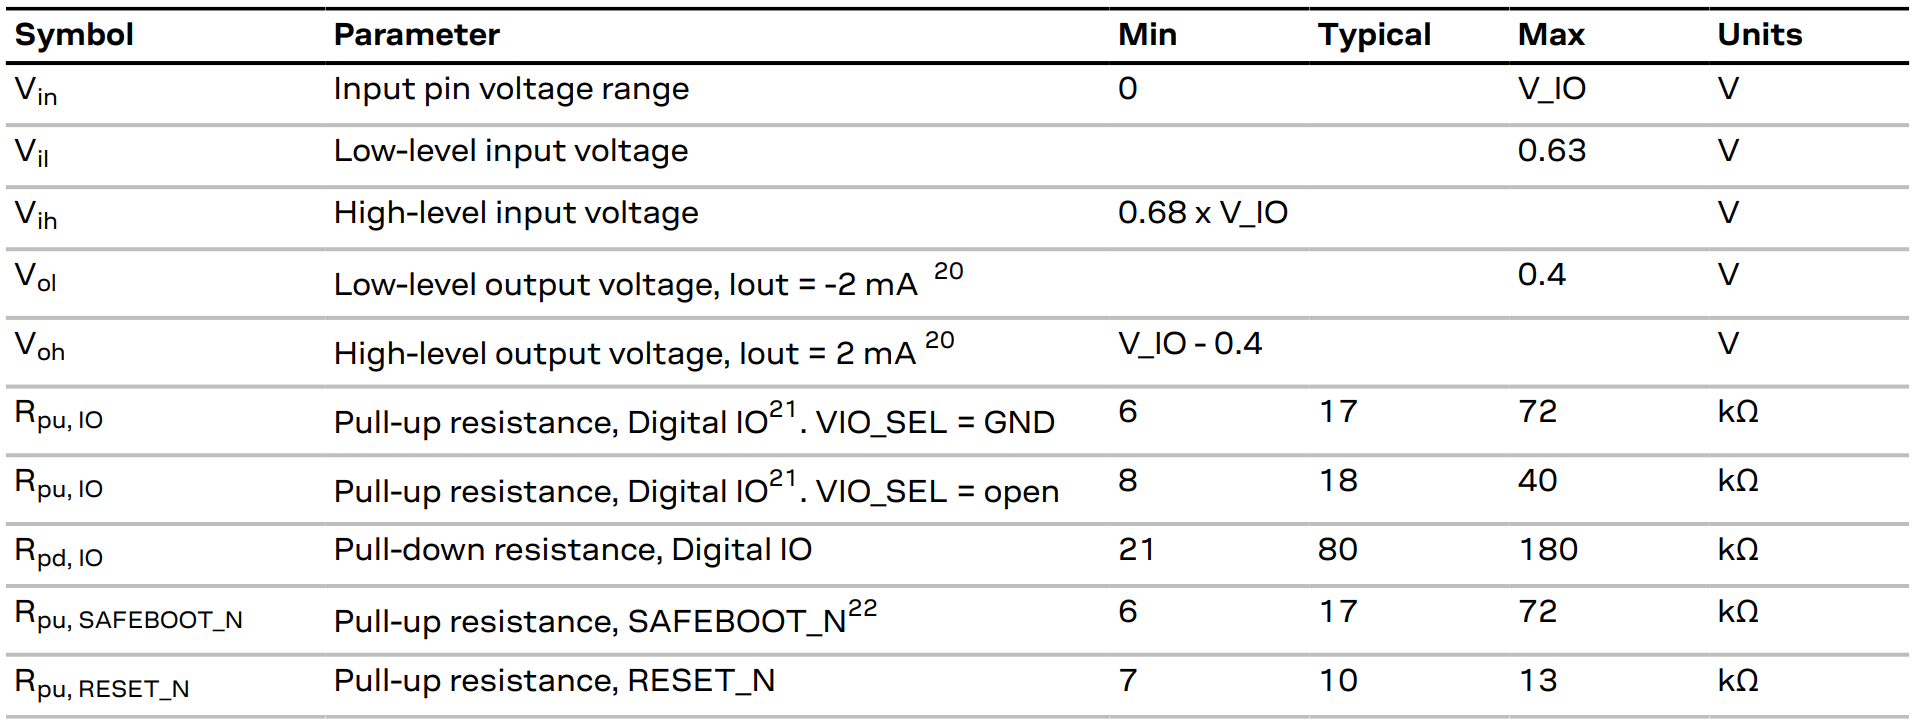
\includegraphics[width=1\textwidth]{Include/Figure/comp/maxm10s_digit_io.png}
\end{subfigure}
	\centering
	\includegraphics[width=1\textwidth]{Include/Figure/comp/maxm10s_digit_io2.png}
\caption{\textit{MAX-M10S} - Digital IO - Source: \cite{MAXM10S}}
\label{tab:maxm10s_digit_io}
\end{table}

\subsubsection{Indicative power requirements:}

Indicative typ. power requirements for the \textit{MAX-M10S} are listed in table \ref{tab:maxm10s_digit_io_current_consum}:

\begin{table}[H]
	\centering
	\includegraphics[width=1\textwidth]{Include/Figure/comp/maxm10s_digit_io_current_consum.png}
\caption{Typical Currents for \SI{3.0}{\volt} Supply at $V_{CC}$ and $V_{IO}$ - Source: \cite{MAXM10S}}
\label{tab:maxm10s_digit_io_current_consum}
\end{table}

Backup current consumption of the \textit{MAX-M10S} is listed in table \ref{tab:maxm10s_back_curr}:

\begin{table}[H]
\begin{subfigure}{\textwidth}
	\centering
	\includegraphics[width=1\textwidth]{Include/Figure/comp/maxm10s_back_curr.png}
\end{subfigure}
	\centering
	\includegraphics[width=1\textwidth]{Include/Figure/comp/maxm10s_back_curr2.png}
\caption{\textit{MAX-M10S} - Backup Currents - Source: \cite{MAXM10S}}
\label{tab:maxm10s_back_curr}
\end{table}

\subsubsection{Communication interfaces:}

The specification of the communication interface of the \textit{MAX-M10S} is described in table \ref{tab:maxm10s_back_curr_i2c_spec}:

\begin{table}[H]
\begin{subfigure}{\textwidth}
	\centering
	\includegraphics[width=1\textwidth]{Include/Figure/comp/maxm10s_back_curr_i2c_spec.png}
\end{subfigure}
	\centering
	\includegraphics[width=1\textwidth]{Include/Figure/comp/maxm10s_back_curr_i2c_spec2.png}
\caption{\textit{MAX-M10S} - Default Interface Settings - Source: \cite{MAXM10S}}
\label{tab:maxm10s_back_curr_i2c_spec}
\end{table}

\subsubsection{Design Recommendations:}
All information about design recommendation are presented in the document "\textit{Standard precision GNSS module - Integration manual}"\cite{MAXM10SINT} from \textsc{u-blox}.
\subsubsection{Design Recommendations - RF interference:}
The biggest concern with \textit{GNSS} is that signal power received to antenna is extremely low compared to other wireless communication signals. In fact, the nominal strength of \textit{GNSS} signal is \SI{-130}{\decibel m}, which is bellow thermal noise floor, making \textit{GNSS} receiver very susceptible to interference from nearby RF sources.\\

For comparison, cellar applications signals strength is approximately \SI{30}{\decibel m} comparing to \textit{GNSS} signals strength value, it is clear that interference issues must be seriously took in consideration during the design phase.\\

RF front-end of \textit{GNSS} receiver is essential to eliminate out-of-band interference from sources such as GSM, CDMA, WCDMA, LTE, Wi-Fi, or Bluetooth. The goal of the RF front-end design is to let pass the inband signal with minimum loss and adding minimum noise while suppressing the out-of-band interference.\\

The \textit{MAX-M10S} integrates a RF front-end block design to keep the highest sensitivity possible. The front-end is also matched to \SI{50}{\ohm}, it also includes a built-in \textit{DC} block, an \textit{LTE Band 13 notch} filter, an \textit{LNA}, and an \textit{SAW} filter.\\

The integration manual still recommends to add an external \textit{SAW} filter to improve the
immunity against RF interference if the application integrates other radio systems. Which is the case for the \textit{LTEWatch} that also integrates a \textit{LTE-M/NB-IoT} modem and antenna. The external \textit{SAW} filter must be selected for an optimal trade-off between sensitivity and immunity.

\subsubsection{Design Recommendations - Power Supply:} \label{sec:gnss_rcvr_sel}
The \textit{MAX-M10S} module power supply must be provided by the VCC and V\_IO pins that can either be connected together or supplied independently  by the system. V\_BCKP is optional and can be use to enable the hardware backup mode that is active when V\_IO supply or both V\_IO and VCC supplies are not supplied.

\begin{enumerate}
\item \textbf{VCC Pin:}
\begin{itemize}
\item Provides power to the core and RF domains and constantly need to be supplied to start-up the receiver or for any operation in continuous mode. The VCC pin is connected to an internal \textit{DCDC} converter that reduce power consumption. The pin is also connected to the RF domain through a ferrit bead.
\item \textbf{\ddl{Note:}} The supply line must not be connected with series resistance greater than \SI{0.2}{\ohm} to avoid voltage ripple due to the dynamic conditions of the current.
\item  The output voltage at VCC\_RF pin is derived from VCC. If supply on VCC is removed, VCC\_RF supply is interrupted.\\
\end{itemize}
\item \textbf{V\_IO  Pin:}
\begin{itemize}
\item All the digital IOs, clock and backup domain are supplied by V\_IO, therefore the current drawn at this pin depends on the loading and activity of the \textit{PIOs} in addition to the \textit{TCXO} consumption.
\item Be aware that a power interruption on this pin will erase the battery-backed RAM (BBR) unless hardware backup is enable (V\_BCKP powered).
\item V\_IO can be supplied with two voltage ranges, \SI{1.8}{\volt} or \SI{3.3}{\volt}. This option is configured with VIO\_SEL pin: Short to \textit{GND} for \SI{1.8}{\volt} designs and left open for \SI{3.3}{\volt} designs.
\item \textbf{\ddl{Note:}} V\_IO supply voltage must never be higher than VCC$+\SI{0.3}{\volt}$\\
\end{itemize}
\item \textbf{V\_BCKP:}
\begin{itemize}
\item Powering this pin is option and is used to enable the hardware backup mode.
\item In this mode, the \textit{RTC} TIME AND THE \textit{gnss} \textit{orbit} data in the \textit{BBR} are maintained.
\item Valid time and \textit{GNSS} \textit{orbit} data at startup improves positioning performance by enabling hot starts, warm starts, and \textit{AssistNow} Autonomous. This ensures faster
time to first fix \textit{(TTFF)} when V\_IO is supplied again.
\item To make these features available, simply power the V\_BCKP with an independent source to ensure backup domain supply when V\_IO is not supplied.\\
\end{itemize}

\item \textbf{Supply Design Examples:}\\
The \textit{integration manual} from \textsc{u-blox} provide voltage supply design examples that are illustrated in figure \ref{fig:maxm10s_volt_supp_ex}:

\begin{figure}[H]
\begin{subfigure}{0.45\textwidth}
\centering
	\includegraphics[width=1\textwidth]{Include/Figure/comp/maxm10s_volt_supp_ex1.png}
	\caption{\centering Common VCC and V\_IO, and supplied V\_BCKP}
\end{subfigure} \hfill
\begin{subfigure}{0.43\textwidth}
\centering
	\includegraphics[width=1\textwidth]{Include/Figure/comp/maxm10s_volt_supp_ex2.png}
	\caption{\centering Common VCC and V\_IO, and V\_BCKP not supplied}
\end{subfigure}\\[10pt]
\begin{subfigure}{0.45\textwidth}
\centering
	\includegraphics[width=1\textwidth]{Include/Figure/comp/maxm10s_volt_supp_ex3.png}
	\caption{\centering Separate VCC and V\_IO, and supplied V\_BCKP}
\end{subfigure} \hfill
\begin{subfigure}{0.45\textwidth}
\centering
	\includegraphics[width=1\textwidth]{Include/Figure/comp/maxm10s_volt_supp_ex4.png}
	\caption{\centering Separate VCC and V\_IO, and V\_BCKP not supplied}
\end{subfigure}
\caption{\textit{MAX-M10S} - Voltage Supply Design Examples - Source: \cite{MAXM10S}}
\label{fig:maxm10s_volt_supp_ex}
\end{figure}
\end{enumerate}


\subsubsection{Design Recommendations - Internal LNA modes:}

The \textit{MAX-M10S} integrated \textit{LNA} can be configured in three operating modes:
\begin{enumerate}
\item \textbf{Normal Gain:} Not recommended for \textit{MAX-M10S} because the already sufficient gain provided by the integrated \textit{LNA}.
\item \textbf{Low Gain:} Default configuration of the \textit{MAX-M10S} for optimized sensitivity and immunity against RF interference.
\item \textbf{Bypass Mode:} Recommended to improve immunity for RF front-end designs with \SI{10}{\decibel} to \SI{15}{\decibel} or higher total external gain. This mode also slightly reduces power consumption.\\
\end{enumerate}

\textbf{\ddl{Note:}} The internal \textit{LNA} mode can be configured at run time in \textit{BBR} and \textit{RAM} of the layers \textit{MAX-M10S} using the configuration item \codeword{CFG-HW-RF_LNA_MODE} follow by a \textbf{reset}.

%-------------------------------------------------------------------------------------

\subsection{Clock Motors: (TITAN T901A/T902A)} \label{sec:mot_sel}
The \textit{LTEWatch} must display time with stepper motors. Those motors were already selected and were provided by the project supervisor \textsc{Medard Rieder}. The next sections presents the specifications and hardware consideration concerning those motors. For more details, full datasheets are in appendix \ref{appendix:motor_t901} and \ref{appendix:motor_t902}.  \\[-20pt]
\subsubsection{Technical Data For TITAN (Bi-Directional) - \textit{T901A}:}

The first motor model is the \textit{T901A},which is a bi-direction single shaft stepper motor design to drive a single clock hand. Figure \ref{fig:motor_single_schem} illustrates the technical data of the \textit{T901A} stepper motor: 

\begin{figure}[H]
	\centering
	\includegraphics[width=1\textwidth]{Include/Figure/comp/motor_single_schem.png}
	\caption{\textit{T901A} - Technical Data For TITAN (Bi-Directional) - Source: \cite{motor1}}
	\label{fig:motor_single_schem}
\end{figure}
\;\\[-55pt]
\subsubsection{Motor Driving Parameters - \textit{T901A}:}

Table \ref{tab:motor_single_motor_driving_param} describes the  \textit{T901A} stepper motor driving parameters: 

\begin{table}[H]
	\centering
	\includegraphics[width=0.70\textwidth]{Include/Figure/comp/motor_single_motor_driving_param.png}
	\caption{\textit{T901A} - Motor Driving Parameters - Source: \cite{motor1}}
	\label{tab:motor_single_motor_driving_param}
\end{table}

\subsubsection{Motor Control Wave Forms - \textit{T901A}:}

Figure \ref{fig:motor_single_wave_form} illustrates wave forms specification for driving the \textit{T901A} motor: 

\begin{figure}[H]
	\centering
	\includegraphics[width=0.8\textwidth]{Include/Figure/comp/motor_single_wave_form.png}
	\caption{\textit{T901A} - Wave Forms - Source: \cite{motor1}}
	\label{fig:motor_single_wave_form}
\end{figure}


\subsubsection{Technical Data For TITAN (Bi-Directional) - \textit{T902A}:}

The second motor model is the \textit{T902A}, which is a bi-direction dual shaft stepper motor design to drive two clock hands.\\

Figure \ref{fig:motor_double_schem} illustrates the technical data of the \textit{T902A} motor: 
\begin{figure}[H]
	\centering
	\includegraphics[width=1\textwidth]{Include/Figure/comp/motor_double_schem.png}
	\caption{\textit{T902A} - Technical Data For TITAN (Bi-Directional) - Source: \cite{motor2}}
	\label{fig:motor_double_schem}
\end{figure}

\pagebreak
\subsubsection{Motor Driving Parameters - \textit{T902A}:}

Table \ref{tab:motor_double_motor_driving_param} describes the \textit{T902A} stepper motor driving parameters: 

\begin{table}[H]
	\centering
	\includegraphics[width=0.8\textwidth]{Include/Figure/comp/motor_double_motor_driving_param.png}
	\caption{\textit{T902A} - Motor Driving Parameters - Source: \cite{motor2}}
	\label{tab:motor_double_motor_driving_param}
\end{table}

\subsubsection{Motor Control Wave Forms - \textit{T902A}:}

Figure \ref{fig:motor_double_wave_form} illustrates wave forms specification for driving the \textit{T902A} stepper motor: 

\begin{figure}[H]
	\centering
	\includegraphics[width=0.8\textwidth]{Include/Figure/comp/motor_double_wave_form.png}
	\caption{\textit{T902A} - Wave Forms - Source: \cite{motor2}}
	\label{fig:motor_double_wave_form}
\end{figure}


%-------------------------------------------------------------------------------------
\pagebreak
\subsection{FTDI USB To UART Interface - FT234XD-R}
In order to add more flexibility to the software development and connectivity of the \textit{LTEWatch} the choice was made to add a \textit{FTDI} \textit{USB To UART} Interface. The datasheet of the \textit{FT234XD-R}\cite{FTDIUSB}, describes the component as a \textit{USB} to serial \textit{UART} interface with size optimized for compact applications. 

\subsubsection{Typical Application Diagram:} \label{sec:ftdi_usb_app}

Figure \ref{fig:FTDIUSB_usb_pwr}, illustrate typical USB bus power configuration for the \textit{ FT234XD-R}:

\begin{figure}[H]
	\centering
	\includegraphics[width=0.75\textwidth]{Include/Figure/comp/FT234XD_R_USB_PWR.png}
	\caption{USB Bus Powered Configuration - Source: \cite{FTDIUSB}}
	\label{fig:FTDIUSB_usb_pwr}
\end{figure}

\subsubsection{Recommended Operating Conditions:}
Recommended conditions for the \textit{FT234XD-R} are presented in table \ref{tab:FTDIUSB_rec_op}:
\begin{table}[H]
\centering
\begin{tabularx}{\textwidth}{|X|c|c|c|c|c|c|}
\hline
\textbf{Parameter} & \textbf{Conditions} & \textbf{ID} & \textbf{MIN} & \textbf{TYP} & \textbf{MAX}        & \textbf{UNIT} \\\hline
VCC Operating Supply Voltag & Normal Operation & VCC & $2.97$ & $5$ & $5.5$ &\si{\volt}\\\hline
VCCIO Operating Supply Voltage & - & VCC2 & $1.62$ & - & $3.63$ & \si{\volt}\\\hline
Operating Supply Current & Normal Operation & Icc1 & $6.5$ & $8$ & $8.3$ & \si{\milli\ampere}\\\hline
Operating Supply Current & USB Suspend & Icc2 & - & $125$ & - & \si{\micro\ampere}\\\hline
3V3 regulator output & - & 3V3 & $2.97$ & $3.3$ & $3.63$ & \si{\volt}\\\hline
\end{tabularx}
\caption{Recommended Operating Conditions - Source: \textit{FT234XD-R}\cite{FTDIUSB}}
\label{tab:FTDIUSB_rec_op}
\end{table}
\;\\[-60pt]
\subsubsection{Absolute Maximum Ratings:}
Absolute maximum ratings for the \textit{FT234XD-R} are presented in table \ref{tab:FTDIUSB_abs_max}:

\begin{table}[H]
\centering
\begin{tabularx}{\textwidth}{|X|c|c|c|}
\hline
\textbf{Parameter} & \textbf{MIN} & \textbf{MAX} & \textbf{UNIT} \\\hline
Storage Temperature & $-65$ & $150$ & \si{\celsius}\\\hline
Ambient Operating Temperature (Power Applied) & $-40$ & $85$ & \si{\celsius}\\\hline
VCC Supply Voltage & $-0.3$ & $+5.5$ & \si{\volt}\\\hline
VCCIO IO Voltage & $-0.3$ & $+4.0$ & \si{\volt}\\\hline
DC Input Voltage – USBDP and USBDM & $-0.5$ & $+3.63$ & \si{\volt}\\\hline
DC Input Voltage – High Impedance Bi-directional (powered from VCCIO) & $-0.3$ & $+5.8$ & \si{\volt}\\\hline
DC Output Current – Outputs & - & $22$ & \si{\milli\ampere}\\\hline
\end{tabularx}
\caption{Absolute maximum ratings - Source: \textit{FT234XD-R}\cite{FTDIUSB}}
\label{tab:FTDIUSB_abs_max}
\end{table}
\;\\[-60pt]
\subsubsection{Features:}

The datasheet of the \textit{FT234XD-R}\cite{FTDIUSB} \textit{USB} to \textit{BASIC UART} IC provides the following features:

\begin{itemize}
\item \textbf{Overview:}
\begin{itemize}
\item Single chip data interface from \textit{USB} to asynchronous data transfer
\item The chip handles entire \textit{USB} protocol and does not require any specific firmware programming
\item Fully integrated 2048 byte multi-timeprogrammable (MTP) memory, storing device descriptors and CBUS I/O configuration specific firmware programming required
\item Fully integrated clock generation with no external crystal required
\end{itemize}
\item \textbf{Performances:}
\begin{itemize}
\item Data transfer rates from \SI{300}{baud} baud to \SI{3}{\mega baud} (\textit{RS422}, \textit{RS485}, and \textit{RS232}) at TTL levels
\item \SI{512}{byte} receive buffer and \SI{512}{byte} transmit buffer
\end{itemize}
\item \textbf{Complementary features:}
\begin{itemize}
\item FTDI’s royalty-free Virtual Com Port (\textit{VCP}) and Direct (\textit{D2XX}) drivers
\item Configurable \textit{CBUS} I/O pin
\item \textit{TX} and \textit{RX} LED drive signals
\item \textit{UART} interface support for $7$ or $8$ data bits, $1$ or $2$ stop bits and \textit{odd} / \textit{even} / \textit{mark} / \textit{space} / \textit{no parity}
\item USB Battery Charging Detection
\item Device supplied pre-programmed with unique \textit{USB} serial number
\item USB Power Configurations:
\begin{itemize}
\item bus-powered
\item self-powered
\item bus-powered with power switching
\end{itemize} 
\item Integrated \SI{+3.3}{\volt} level converter for \textit{USB I/O}
\item Integrated \textit{power-on-reset} circuit
\end{itemize}
\item \textbf{Size and package:} \textit{DFN} 12 pin package ($\SI{3}{\milli\meter} \times \SI{3}{\milli\meter}$) 
\end{itemize}

\pagebreak


\subsubsection{Design Recommendations:} \label{sec:ftdi_sel}

Because the \textit{FT234XD-R} is a \textit{USB} to \textit{UART} interface, basic rules for USB bus  power devices must be respected. Those basic rules are provided in the datasheet of the \textit{FT234XD-R}\cite{FTDIUSB} and are as follows:

\begin{enumerate}
\item On \textit{USB} plug-in, the device should draw no more current than \SI{100}{\milli\ampere}
\item In \textit{USB} Suspend mode the device should draw no more than \SI{2.5}{\milli\ampere}
\item A bus powered high power \textit{USB} device (one that draws more than \SI{100}{\milli\ampere}) should use the \textit{CBUS} pin configured as \textit{PWREN\#} and use it to keep the current below \SI{100}{\milli\ampere} on plug-in and \SI{2.5}{\milli\ampere} on \textit{USB} suspend
\item A device that consumes more than \SI{100}{\milli\ampere} cannot be plugged into a \textit{USB} bus powered hub
\item No device can draw more than \SI{500}{\milli\ampere} from the \textit{USB} bus
\end{enumerate}

\subsection{Components Package Type and Size Selection} \label{sec:comp_size_select}
The prototype board integrates the \textit{nRF9160 SiP} from \textsc{Nordic Semi.}. This \textit{SiP} is only available as a \textit{LGA} package, which is not easy to assemble. To ensure the correct assembly of the prototype \textit{PCBs}, it was agreed with the project manager \textsc{Rieder Medard} to order them fully assembled in-house by \textsc{Euro Circuits}. As assembly is no longer a constraint, it is possible to select tiny package type such as \textit{BGA}  in order to design a compact device. That's why many components have been selected in tiny difficult to assemble packages.\\

Concerning all passive components like resistors, capacitors or inductors, the opposite approach was chosen. The \textit{LTEWatch} board is a prototype, it is reasonable to expect that modifications will probably be necessary. To ensure easier modification of the passive components, it was decided to select these components in \textbf{0603} size packages. This package size is the smallest size that I've always been comfortable replacing and soldering without too much difficulty. This components can easily be replaced by \textbf{0402} size packages for the final round version of the \textit{LTEWatch}.

\end{document}
